\documentclass[xcolor=dvipsnames,table]{beamer}
\usepackage[english, spanish, galician]{babel} 
\usepackage[utf8]{inputenc}
\usepackage{caption}
\usepackage{graphicx}
\usepackage{subfigure}
\usepackage{booktabs}
\usepackage{url}
\usepackage{eurosym}
\usepackage{rotating}
\usepackage{amsmath}
\usepackage{multirow}
\usepackage{colortbl}
\usepackage{comment}

\usepackage{color}

\usepackage{tikz}
\usetikzlibrary{calc}
\usepackage{mathrsfs}
\usepackage{animate}
\usepackage{ulem}
\usepackage[labelformat=empty]{caption}
%\usepackage{xmpmulti}
\usepackage{multimedia}
\usepackage{media9}
\definecolor{AliceBlue}{rgb}{0.94,0.97,1.00}
\definecolor{AntiqueWhite1}{rgb}{1.00,0.94,0.86}
\definecolor{AntiqueWhite2}{rgb}{0.93,0.87,0.80}
\definecolor{AntiqueWhite3}{rgb}{0.80,0.75,0.69}
\definecolor{AntiqueWhite4}{rgb}{0.55,0.51,0.47}
\definecolor{AntiqueWhite}{rgb}{0.98,0.92,0.84}
\definecolor{BlanchedAlmond}{rgb}{1.00,0.92,0.80}
\definecolor{BlueViolet}{rgb}{0.54,0.17,0.89}
\definecolor{CadetBlue1}{rgb}{0.60,0.96,1.00}
\definecolor{CadetBlue2}{rgb}{0.56,0.90,0.93}
\definecolor{CadetBlue3}{rgb}{0.48,0.77,0.80}
\definecolor{CadetBlue4}{rgb}{0.33,0.53,0.55}
\definecolor{CadetBlue}{rgb}{0.37,0.62,0.63}
\definecolor{CornflowerBlue}{rgb}{0.39,0.58,0.93}
\definecolor{DarkBlue}{rgb}{0.00,0.00,0.55}
\definecolor{DarkCyan}{rgb}{0.00,0.55,0.55}
\definecolor{DarkGoldenrod1}{rgb}{1.00,0.73,0.06}
\definecolor{DarkGoldenrod2}{rgb}{0.93,0.68,0.05}
\definecolor{DarkGoldenrod3}{rgb}{0.80,0.58,0.05}
\definecolor{DarkGoldenrod4}{rgb}{0.55,0.40,0.03}
\definecolor{DarkGoldenrod}{rgb}{0.72,0.53,0.04}
\definecolor{DarkGray}{rgb}{0.66,0.66,0.66}
\definecolor{DarkGreen}{rgb}{0.00,0.39,0.00}
\definecolor{DarkGrey}{rgb}{0.66,0.66,0.66}
\definecolor{DarkKhaki}{rgb}{0.74,0.72,0.42}
\definecolor{DarkMagenta}{rgb}{0.55,0.00,0.55}
\definecolor{DarkOliveGreen1}{rgb}{0.79,1.00,0.44}
\definecolor{DarkOliveGreen2}{rgb}{0.74,0.93,0.41}
\definecolor{DarkOliveGreen3}{rgb}{0.64,0.80,0.35}
\definecolor{DarkOliveGreen4}{rgb}{0.43,0.55,0.24}
\definecolor{DarkOliveGreen}{rgb}{0.33,0.42,0.18}
\definecolor{DarkOrange1}{rgb}{1.00,0.50,0.00}
\definecolor{DarkOrange2}{rgb}{0.93,0.46,0.00}
\definecolor{DarkOrange3}{rgb}{0.80,0.40,0.00}
\definecolor{DarkOrange4}{rgb}{0.55,0.27,0.00}
\definecolor{DarkOrange}{rgb}{1.00,0.55,0.00}
\definecolor{DarkOrchid1}{rgb}{0.75,0.24,1.00}
\definecolor{DarkOrchid2}{rgb}{0.70,0.23,0.93}
\definecolor{DarkOrchid3}{rgb}{0.60,0.20,0.80}
\definecolor{DarkOrchid4}{rgb}{0.41,0.13,0.55}
\definecolor{DarkOrchid}{rgb}{0.60,0.20,0.80}
\definecolor{DarkRed}{rgb}{0.55,0.00,0.00}
\definecolor{DarkSalmon}{rgb}{0.91,0.59,0.48}
\definecolor{DarkSeaGreen1}{rgb}{0.76,1.00,0.76}
\definecolor{DarkSeaGreen2}{rgb}{0.71,0.93,0.71}
\definecolor{DarkSeaGreen3}{rgb}{0.61,0.80,0.61}
\definecolor{DarkSeaGreen4}{rgb}{0.41,0.55,0.41}
\definecolor{DarkSeaGreen}{rgb}{0.56,0.74,0.56}
\definecolor{DarkSlateBlue}{rgb}{0.28,0.24,0.55}
\definecolor{DarkSlateGray1}{rgb}{0.59,1.00,1.00}
\definecolor{DarkSlateGray2}{rgb}{0.55,0.93,0.93}
\definecolor{DarkSlateGray3}{rgb}{0.47,0.80,0.80}
\definecolor{DarkSlateGray4}{rgb}{0.32,0.55,0.55}
\definecolor{DarkSlateGray}{rgb}{0.18,0.31,0.31}
\definecolor{DarkSlateGrey}{rgb}{0.18,0.31,0.31}
\definecolor{DarkTurquoise}{rgb}{0.00,0.81,0.82}
\definecolor{DarkViolet}{rgb}{0.58,0.00,0.83}
\definecolor{DeepPink1}{rgb}{1.00,0.08,0.58}
\definecolor{DeepPink2}{rgb}{0.93,0.07,0.54}
\definecolor{DeepPink3}{rgb}{0.80,0.06,0.46}
\definecolor{DeepPink4}{rgb}{0.55,0.04,0.31}
\definecolor{DeepPink}{rgb}{1.00,0.08,0.58}
\definecolor{DeepSkyBlue1}{rgb}{0.00,0.75,1.00}
\definecolor{DeepSkyBlue2}{rgb}{0.00,0.70,0.93}
\definecolor{DeepSkyBlue3}{rgb}{0.00,0.60,0.80}
\definecolor{DeepSkyBlue4}{rgb}{0.00,0.41,0.55}
\definecolor{DeepSkyBlue}{rgb}{0.00,0.75,1.00}
\definecolor{DimGray}{rgb}{0.41,0.41,0.41}
\definecolor{DimGrey}{rgb}{0.41,0.41,0.41}
\definecolor{DodgerBlue1}{rgb}{0.12,0.56,1.00}
\definecolor{DodgerBlue2}{rgb}{0.11,0.53,0.93}
\definecolor{DodgerBlue3}{rgb}{0.09,0.45,0.80}
\definecolor{DodgerBlue4}{rgb}{0.06,0.31,0.55}
\definecolor{DodgerBlue}{rgb}{0.12,0.56,1.00}
\definecolor{FloralWhite}{rgb}{1.00,0.98,0.94}
\definecolor{ForestGreen}{rgb}{0.13,0.55,0.13}
\definecolor{GhostWhite}{rgb}{0.97,0.97,1.00}
\definecolor{GreenYellow}{rgb}{0.68,1.00,0.18}
\definecolor{HotPink1}{rgb}{1.00,0.43,0.71}
\definecolor{HotPink2}{rgb}{0.93,0.42,0.65}
\definecolor{HotPink3}{rgb}{0.80,0.38,0.56}
\definecolor{HotPink4}{rgb}{0.55,0.23,0.38}
\definecolor{HotPink}{rgb}{1.00,0.41,0.71}
\definecolor{IndianRed1}{rgb}{1.00,0.42,0.42}
\definecolor{IndianRed2}{rgb}{0.93,0.39,0.39}
\definecolor{IndianRed3}{rgb}{0.80,0.33,0.33}
\definecolor{IndianRed4}{rgb}{0.55,0.23,0.23}
\definecolor{IndianRed}{rgb}{0.80,0.36,0.36}
\definecolor{LavenderBlush1}{rgb}{1.00,0.94,0.96}
\definecolor{LavenderBlush2}{rgb}{0.93,0.88,0.90}
\definecolor{LavenderBlush3}{rgb}{0.80,0.76,0.77}
\definecolor{LavenderBlush4}{rgb}{0.55,0.51,0.53}
\definecolor{LavenderBlush}{rgb}{1.00,0.94,0.96}
\definecolor{LawnGreen}{rgb}{0.49,0.99,0.00}
\definecolor{LemonChiffon1}{rgb}{1.00,0.98,0.80}
\definecolor{LemonChiffon2}{rgb}{0.93,0.91,0.75}
\definecolor{LemonChiffon3}{rgb}{0.80,0.79,0.65}
\definecolor{LemonChiffon4}{rgb}{0.55,0.54,0.44}
\definecolor{LemonChiffon}{rgb}{1.00,0.98,0.80}
\definecolor{LightBlue1}{rgb}{0.75,0.94,1.00}
\definecolor{LightBlue2}{rgb}{0.70,0.87,0.93}
\definecolor{LightBlue3}{rgb}{0.60,0.75,0.80}
\definecolor{LightBlue4}{rgb}{0.41,0.51,0.55}
\definecolor{LightBlue}{rgb}{0.68,0.85,0.90}
\definecolor{LightCoral}{rgb}{0.94,0.50,0.50}
\definecolor{LightCyan1}{rgb}{0.88,1.00,1.00}
\definecolor{LightCyan2}{rgb}{0.82,0.93,0.93}
\definecolor{LightCyan3}{rgb}{0.71,0.80,0.80}
\definecolor{LightCyan4}{rgb}{0.48,0.55,0.55}
\definecolor{LightCyan}{rgb}{0.88,1.00,1.00}
\definecolor{LightGoldenrod1}{rgb}{1.00,0.93,0.55}
\definecolor{LightGoldenrod2}{rgb}{0.93,0.86,0.51}
\definecolor{LightGoldenrod3}{rgb}{0.80,0.75,0.44}
\definecolor{LightGoldenrod4}{rgb}{0.55,0.51,0.30}
\definecolor{LightGoldenrodYellow}{rgb}{0.98,0.98,0.82}
\definecolor{LightGoldenrod}{rgb}{0.93,0.87,0.51}
\definecolor{LightGray}{rgb}{0.83,0.83,0.83}
\definecolor{LightGreen}{rgb}{0.56,0.93,0.56}
\definecolor{LightGrey}{rgb}{0.83,0.83,0.83}
\definecolor{LightPink1}{rgb}{1.00,0.68,0.73}
\definecolor{LightPink2}{rgb}{0.93,0.64,0.68}
\definecolor{LightPink3}{rgb}{0.80,0.55,0.58}
\definecolor{LightPink4}{rgb}{0.55,0.37,0.40}
\definecolor{LightPink}{rgb}{1.00,0.71,0.76}
\definecolor{LightSalmon1}{rgb}{1.00,0.63,0.48}
\definecolor{LightSalmon2}{rgb}{0.93,0.58,0.45}
\definecolor{LightSalmon3}{rgb}{0.80,0.51,0.38}
\definecolor{LightSalmon4}{rgb}{0.55,0.34,0.26}
\definecolor{LightSalmon}{rgb}{1.00,0.63,0.48}
\definecolor{LightSeaGreen}{rgb}{0.13,0.70,0.67}
\definecolor{LightSkyBlue1}{rgb}{0.69,0.89,1.00}
\definecolor{LightSkyBlue2}{rgb}{0.64,0.83,0.93}
\definecolor{LightSkyBlue3}{rgb}{0.55,0.71,0.80}
\definecolor{LightSkyBlue4}{rgb}{0.38,0.48,0.55}
\definecolor{LightSkyBlue}{rgb}{0.53,0.81,0.98}
\definecolor{LightSlateBlue}{rgb}{0.52,0.44,1.00}
\definecolor{LightSlateGray}{rgb}{0.47,0.53,0.60}
\definecolor{LightSlateGrey}{rgb}{0.47,0.53,0.60}
\definecolor{LightSteelBlue1}{rgb}{0.79,0.88,1.00}
\definecolor{LightSteelBlue2}{rgb}{0.74,0.82,0.93}
\definecolor{LightSteelBlue3}{rgb}{0.64,0.71,0.80}
\definecolor{LightSteelBlue4}{rgb}{0.43,0.48,0.55}
\definecolor{LightSteelBlue}{rgb}{0.69,0.77,0.87}
\definecolor{LightYellow1}{rgb}{1.00,1.00,0.88}
\definecolor{LightYellow2}{rgb}{0.93,0.93,0.82}
\definecolor{LightYellow3}{rgb}{0.80,0.80,0.71}
\definecolor{LightYellow4}{rgb}{0.55,0.55,0.48}
\definecolor{LightYellow}{rgb}{1.00,1.00,0.88}
\definecolor{LimeGreen}{rgb}{0.20,0.80,0.20}
\definecolor{MediumAquamarine}{rgb}{0.40,0.80,0.67}
\definecolor{MediumBlue}{rgb}{0.00,0.00,0.80}
\definecolor{MediumOrchid1}{rgb}{0.88,0.40,1.00}
\definecolor{MediumOrchid2}{rgb}{0.82,0.37,0.93}
\definecolor{MediumOrchid3}{rgb}{0.71,0.32,0.80}
\definecolor{MediumOrchid4}{rgb}{0.48,0.22,0.55}
\definecolor{MediumOrchid}{rgb}{0.73,0.33,0.83}
\definecolor{MediumPurple1}{rgb}{0.67,0.51,1.00}
\definecolor{MediumPurple2}{rgb}{0.62,0.47,0.93}
\definecolor{MediumPurple3}{rgb}{0.54,0.41,0.80}
\definecolor{MediumPurple4}{rgb}{0.36,0.28,0.55}
\definecolor{MediumPurple}{rgb}{0.58,0.44,0.86}
\definecolor{MediumSeaGreen}{rgb}{0.24,0.70,0.44}
\definecolor{MediumSlateBlue}{rgb}{0.48,0.41,0.93}
\definecolor{MediumSpringGreen}{rgb}{0.00,0.98,0.60}
\definecolor{MediumTurquoise}{rgb}{0.28,0.82,0.80}
\definecolor{MediumVioletRed}{rgb}{0.78,0.08,0.52}
\definecolor{MidnightBlue}{rgb}{0.10,0.10,0.44}
\definecolor{MintCream}{rgb}{0.96,1.00,0.98}
\definecolor{MistyRose1}{rgb}{1.00,0.89,0.88}
\definecolor{MistyRose2}{rgb}{0.93,0.84,0.82}
\definecolor{MistyRose3}{rgb}{0.80,0.72,0.71}
\definecolor{MistyRose4}{rgb}{0.55,0.49,0.48}
\definecolor{MistyRose}{rgb}{1.00,0.89,0.88}
\definecolor{NavajoWhite1}{rgb}{1.00,0.87,0.68}
\definecolor{NavajoWhite2}{rgb}{0.93,0.81,0.63}
\definecolor{NavajoWhite3}{rgb}{0.80,0.70,0.55}
\definecolor{NavajoWhite4}{rgb}{0.55,0.47,0.37}
\definecolor{NavajoWhite}{rgb}{1.00,0.87,0.68}
\definecolor{NavyBlue}{rgb}{0.00,0.00,0.50}
\definecolor{OldLace}{rgb}{0.99,0.96,0.90}
\definecolor{OliveDrab1}{rgb}{0.75,1.00,0.24}
\definecolor{OliveDrab2}{rgb}{0.70,0.93,0.23}
\definecolor{OliveDrab3}{rgb}{0.60,0.80,0.20}
\definecolor{OliveDrab4}{rgb}{0.41,0.55,0.13}
\definecolor{OliveDrab}{rgb}{0.42,0.56,0.14}
\definecolor{OrangeRed1}{rgb}{1.00,0.27,0.00}
\definecolor{OrangeRed2}{rgb}{0.93,0.25,0.00}
\definecolor{OrangeRed3}{rgb}{0.80,0.22,0.00}
\definecolor{OrangeRed4}{rgb}{0.55,0.15,0.00}
\definecolor{OrangeRed}{rgb}{1.00,0.27,0.00}
\definecolor{PaleGoldenrod}{rgb}{0.93,0.91,0.67}
\definecolor{PaleGreen1}{rgb}{0.60,1.00,0.60}
\definecolor{PaleGreen2}{rgb}{0.56,0.93,0.56}
\definecolor{PaleGreen3}{rgb}{0.49,0.80,0.49}
\definecolor{PaleGreen4}{rgb}{0.33,0.55,0.33}
\definecolor{PaleGreen}{rgb}{0.60,0.98,0.60}
\definecolor{PaleTurquoise1}{rgb}{0.73,1.00,1.00}
\definecolor{PaleTurquoise2}{rgb}{0.68,0.93,0.93}
\definecolor{PaleTurquoise3}{rgb}{0.59,0.80,0.80}
\definecolor{PaleTurquoise4}{rgb}{0.40,0.55,0.55}
\definecolor{PaleTurquoise}{rgb}{0.69,0.93,0.93}
\definecolor{PaleVioletRed1}{rgb}{1.00,0.51,0.67}
\definecolor{PaleVioletRed2}{rgb}{0.93,0.47,0.62}
\definecolor{PaleVioletRed3}{rgb}{0.80,0.41,0.54}
\definecolor{PaleVioletRed4}{rgb}{0.55,0.28,0.36}
\definecolor{PaleVioletRed}{rgb}{0.86,0.44,0.58}
\definecolor{PapayaWhip}{rgb}{1.00,0.94,0.84}
\definecolor{PeachPuff1}{rgb}{1.00,0.85,0.73}
\definecolor{PeachPuff2}{rgb}{0.93,0.80,0.68}
\definecolor{PeachPuff3}{rgb}{0.80,0.69,0.58}
\definecolor{PeachPuff4}{rgb}{0.55,0.47,0.40}
\definecolor{PeachPuff}{rgb}{1.00,0.85,0.73}
\definecolor{PowderBlue}{rgb}{0.69,0.88,0.90}
\definecolor{RosyBrown1}{rgb}{1.00,0.76,0.76}
\definecolor{RosyBrown2}{rgb}{0.93,0.71,0.71}
\definecolor{RosyBrown3}{rgb}{0.80,0.61,0.61}
\definecolor{RosyBrown4}{rgb}{0.55,0.41,0.41}
\definecolor{RosyBrown}{rgb}{0.74,0.56,0.56}
\definecolor{RoyalBlue1}{rgb}{0.28,0.46,1.00}
\definecolor{RoyalBlue2}{rgb}{0.26,0.43,0.93}
\definecolor{RoyalBlue3}{rgb}{0.23,0.37,0.80}
\definecolor{RoyalBlue4}{rgb}{0.15,0.25,0.55}
\definecolor{RoyalBlue}{rgb}{0.25,0.41,0.88}
\definecolor{SaddleBrown}{rgb}{0.55,0.27,0.07}
\definecolor{SandyBrown}{rgb}{0.96,0.64,0.38}
\definecolor{SeaGreen1}{rgb}{0.33,1.00,0.62}
\definecolor{SeaGreen2}{rgb}{0.31,0.93,0.58}
\definecolor{SeaGreen3}{rgb}{0.26,0.80,0.50}
\definecolor{SeaGreen4}{rgb}{0.18,0.55,0.34}
\definecolor{SeaGreen}{rgb}{0.18,0.55,0.34}
\definecolor{SkyBlue1}{rgb}{0.53,0.81,1.00}
\definecolor{SkyBlue2}{rgb}{0.49,0.75,0.93}
\definecolor{SkyBlue3}{rgb}{0.42,0.65,0.80}
\definecolor{SkyBlue4}{rgb}{0.29,0.44,0.55}
\definecolor{SkyBlue}{rgb}{0.53,0.81,0.92}
\definecolor{SlateBlue1}{rgb}{0.51,0.44,1.00}
\definecolor{SlateBlue2}{rgb}{0.48,0.40,0.93}
\definecolor{SlateBlue3}{rgb}{0.41,0.35,0.80}
\definecolor{SlateBlue4}{rgb}{0.28,0.24,0.55}
\definecolor{SlateBlue}{rgb}{0.42,0.35,0.80}
\definecolor{SlateGray1}{rgb}{0.78,0.89,1.00}
\definecolor{SlateGray2}{rgb}{0.73,0.83,0.93}
\definecolor{SlateGray3}{rgb}{0.62,0.71,0.80}
\definecolor{SlateGray4}{rgb}{0.42,0.48,0.55}
\definecolor{SlateGray}{rgb}{0.44,0.50,0.56}
\definecolor{SlateGrey}{rgb}{0.44,0.50,0.56}
\definecolor{SpringGreen1}{rgb}{0.00,1.00,0.50}
\definecolor{SpringGreen2}{rgb}{0.00,0.93,0.46}
\definecolor{SpringGreen3}{rgb}{0.00,0.80,0.40}
\definecolor{SpringGreen4}{rgb}{0.00,0.55,0.27}
\definecolor{SpringGreen}{rgb}{0.00,1.00,0.50}
\definecolor{SteelBlue1}{rgb}{0.39,0.72,1.00}
\definecolor{SteelBlue2}{rgb}{0.36,0.67,0.93}
\definecolor{SteelBlue3}{rgb}{0.31,0.58,0.80}
\definecolor{SteelBlue4}{rgb}{0.21,0.39,0.55}
\definecolor{SteelBlue}{rgb}{0.27,0.51,0.71}
\definecolor{VioletRed1}{rgb}{1.00,0.24,0.59}
\definecolor{VioletRed2}{rgb}{0.93,0.23,0.55}
\definecolor{VioletRed3}{rgb}{0.80,0.20,0.47}
\definecolor{VioletRed4}{rgb}{0.55,0.13,0.32}
\definecolor{VioletRed}{rgb}{0.82,0.13,0.56}
\definecolor{WhiteSmoke}{rgb}{0.96,0.96,0.96}
\definecolor{YellowGreen}{rgb}{0.60,0.80,0.20}
\definecolor{aliceblue}{rgb}{0.94,0.97,1.00}
\definecolor{antiquewhite}{rgb}{0.98,0.92,0.84}
\definecolor{aquamarine1}{rgb}{0.50,1.00,0.83}
\definecolor{aquamarine2}{rgb}{0.46,0.93,0.78}
\definecolor{aquamarine3}{rgb}{0.40,0.80,0.67}
\definecolor{aquamarine4}{rgb}{0.27,0.55,0.45}
\definecolor{aquamarine}{rgb}{0.50,1.00,0.83}
\definecolor{azure1}{rgb}{0.94,1.00,1.00}
\definecolor{azure2}{rgb}{0.88,0.93,0.93}
\definecolor{azure3}{rgb}{0.76,0.80,0.80}
\definecolor{azure4}{rgb}{0.51,0.55,0.55}
\definecolor{azure}{rgb}{0.94,1.00,1.00}
\definecolor{beige}{rgb}{0.96,0.96,0.86}
\definecolor{bisque1}{rgb}{1.00,0.89,0.77}
\definecolor{bisque2}{rgb}{0.93,0.84,0.72}
\definecolor{bisque3}{rgb}{0.80,0.72,0.62}
\definecolor{bisque4}{rgb}{0.55,0.49,0.42}
\definecolor{bisque}{rgb}{1.00,0.89,0.77}
\definecolor{black}{rgb}{0.00,0.00,0.00}
\definecolor{blanchedalmond}{rgb}{1.00,0.92,0.80}
\definecolor{blue1}{rgb}{0.00,0.00,1.00}
\definecolor{blue2}{rgb}{0.00,0.00,0.93}
\definecolor{blue3}{rgb}{0.00,0.00,0.80}
\definecolor{blue4}{rgb}{0.00,0.00,0.55}
\definecolor{blueviolet}{rgb}{0.54,0.17,0.89}
\definecolor{blue}{rgb}{0.00,0.00,1.00}
\definecolor{brown1}{rgb}{1.00,0.25,0.25}
\definecolor{brown2}{rgb}{0.93,0.23,0.23}
\definecolor{brown3}{rgb}{0.80,0.20,0.20}
\definecolor{brown4}{rgb}{0.55,0.14,0.14}
\definecolor{brown}{rgb}{0.65,0.16,0.16}
\definecolor{burlywood1}{rgb}{1.00,0.83,0.61}
\definecolor{burlywood2}{rgb}{0.93,0.77,0.57}
\definecolor{burlywood3}{rgb}{0.80,0.67,0.49}
\definecolor{burlywood4}{rgb}{0.55,0.45,0.33}
\definecolor{burlywood}{rgb}{0.87,0.72,0.53}
\definecolor{cadetblue}{rgb}{0.37,0.62,0.63}
\definecolor{chartreuse1}{rgb}{0.50,1.00,0.00}
\definecolor{chartreuse2}{rgb}{0.46,0.93,0.00}
\definecolor{chartreuse3}{rgb}{0.40,0.80,0.00}
\definecolor{chartreuse4}{rgb}{0.27,0.55,0.00}
\definecolor{chartreuse}{rgb}{0.50,1.00,0.00}
\definecolor{chocolate1}{rgb}{1.00,0.50,0.14}
\definecolor{chocolate2}{rgb}{0.93,0.46,0.13}
\definecolor{chocolate3}{rgb}{0.80,0.40,0.11}
\definecolor{chocolate4}{rgb}{0.55,0.27,0.07}
\definecolor{chocolate}{rgb}{0.82,0.41,0.12}
\definecolor{coral1}{rgb}{1.00,0.45,0.34}
\definecolor{coral2}{rgb}{0.93,0.42,0.31}
\definecolor{coral3}{rgb}{0.80,0.36,0.27}
\definecolor{coral4}{rgb}{0.55,0.24,0.18}
\definecolor{coral}{rgb}{1.00,0.50,0.31}
\definecolor{cornflowerblue}{rgb}{0.39,0.58,0.93}
\definecolor{cornsilk1}{rgb}{1.00,0.97,0.86}
\definecolor{cornsilk2}{rgb}{0.93,0.91,0.80}
\definecolor{cornsilk3}{rgb}{0.80,0.78,0.69}
\definecolor{cornsilk4}{rgb}{0.55,0.53,0.47}
\definecolor{cornsilk}{rgb}{1.00,0.97,0.86}
\definecolor{cyan1}{rgb}{0.00,1.00,1.00}
\definecolor{cyan2}{rgb}{0.00,0.93,0.93}
\definecolor{cyan3}{rgb}{0.00,0.80,0.80}
\definecolor{cyan4}{rgb}{0.00,0.55,0.55}
\definecolor{cyan}{rgb}{0.00,1.00,1.00}
\definecolor{darkblue}{rgb}{0.00,0.00,0.55}
\definecolor{darkcyan}{rgb}{0.00,0.55,0.55}
\definecolor{darkgoldenrod}{rgb}{0.72,0.53,0.04}
\definecolor{darkgray}{rgb}{0.66,0.66,0.66}
\definecolor{darkgreen}{rgb}{0.00,0.39,0.00}
\definecolor{darkgrey}{rgb}{0.66,0.66,0.66}
\definecolor{darkkhaki}{rgb}{0.74,0.72,0.42}
\definecolor{darkmagenta}{rgb}{0.55,0.00,0.55}
\definecolor{darkolive}{rgb}{0.33,0.42,0.18}
\definecolor{darkorange}{rgb}{1.00,0.55,0.00}
\definecolor{darkorchid}{rgb}{0.60,0.20,0.80}
\definecolor{darkred}{rgb}{0.55,0.00,0.00}
\definecolor{darksalmon}{rgb}{0.91,0.59,0.48}
\definecolor{darksea}{rgb}{0.56,0.74,0.56}
\definecolor{darkslate}{rgb}{0.18,0.31,0.31}
\definecolor{darkslate}{rgb}{0.18,0.31,0.31}
\definecolor{darkslate}{rgb}{0.28,0.24,0.55}
\definecolor{darkturquoise}{rgb}{0.00,0.81,0.82}
\definecolor{darkviolet}{rgb}{0.58,0.00,0.83}
\definecolor{deeppink}{rgb}{1.00,0.08,0.58}
\definecolor{deepsky}{rgb}{0.00,0.75,1.00}
\definecolor{dimgray}{rgb}{0.41,0.41,0.41}
\definecolor{dimgrey}{rgb}{0.41,0.41,0.41}
\definecolor{dodgerblue}{rgb}{0.12,0.56,1.00}
\definecolor{firebrick1}{rgb}{1.00,0.19,0.19}
\definecolor{firebrick2}{rgb}{0.93,0.17,0.17}
\definecolor{firebrick3}{rgb}{0.80,0.15,0.15}
\definecolor{firebrick4}{rgb}{0.55,0.10,0.10}
\definecolor{firebrick}{rgb}{0.70,0.13,0.13}
\definecolor{floralwhite}{rgb}{1.00,0.98,0.94}
\definecolor{forestgreen}{rgb}{0.13,0.55,0.13}
\definecolor{gainsboro}{rgb}{0.86,0.86,0.86}
\definecolor{ghostwhite}{rgb}{0.97,0.97,1.00}
\definecolor{gold1}{rgb}{1.00,0.84,0.00}
\definecolor{gold2}{rgb}{0.93,0.79,0.00}
\definecolor{gold3}{rgb}{0.80,0.68,0.00}
\definecolor{gold4}{rgb}{0.55,0.46,0.00}
\definecolor{goldenrod1}{rgb}{1.00,0.76,0.15}
\definecolor{goldenrod2}{rgb}{0.93,0.71,0.13}
\definecolor{goldenrod3}{rgb}{0.80,0.61,0.11}
\definecolor{goldenrod4}{rgb}{0.55,0.41,0.08}
\definecolor{goldenrod}{rgb}{0.85,0.65,0.13}
\definecolor{gold}{rgb}{1.00,0.84,0.00}
\definecolor{gray0}{rgb}{0.00,0.00,0.00}
\definecolor{gray100}{rgb}{1.00,1.00,1.00}
\definecolor{gray10}{rgb}{0.10,0.10,0.10}
\definecolor{gray11}{rgb}{0.11,0.11,0.11}
\definecolor{gray12}{rgb}{0.12,0.12,0.12}
\definecolor{gray13}{rgb}{0.13,0.13,0.13}
\definecolor{gray14}{rgb}{0.14,0.14,0.14}
\definecolor{gray15}{rgb}{0.15,0.15,0.15}
\definecolor{gray16}{rgb}{0.16,0.16,0.16}
\definecolor{gray17}{rgb}{0.17,0.17,0.17}
\definecolor{gray18}{rgb}{0.18,0.18,0.18}
\definecolor{gray19}{rgb}{0.19,0.19,0.19}
\definecolor{gray1}{rgb}{0.01,0.01,0.01}
\definecolor{gray20}{rgb}{0.20,0.20,0.20}
\definecolor{gray21}{rgb}{0.21,0.21,0.21}
\definecolor{gray22}{rgb}{0.22,0.22,0.22}
\definecolor{gray23}{rgb}{0.23,0.23,0.23}
\definecolor{gray24}{rgb}{0.24,0.24,0.24}
\definecolor{gray25}{rgb}{0.25,0.25,0.25}
\definecolor{gray26}{rgb}{0.26,0.26,0.26}
\definecolor{gray27}{rgb}{0.27,0.27,0.27}
\definecolor{gray28}{rgb}{0.28,0.28,0.28}
\definecolor{gray29}{rgb}{0.29,0.29,0.29}
\definecolor{gray2}{rgb}{0.02,0.02,0.02}
\definecolor{gray30}{rgb}{0.30,0.30,0.30}
\definecolor{gray31}{rgb}{0.31,0.31,0.31}
\definecolor{gray32}{rgb}{0.32,0.32,0.32}
\definecolor{gray33}{rgb}{0.33,0.33,0.33}
\definecolor{gray34}{rgb}{0.34,0.34,0.34}
\definecolor{gray35}{rgb}{0.35,0.35,0.35}
\definecolor{gray36}{rgb}{0.36,0.36,0.36}
\definecolor{gray37}{rgb}{0.37,0.37,0.37}
\definecolor{gray38}{rgb}{0.38,0.38,0.38}
\definecolor{gray39}{rgb}{0.39,0.39,0.39}
\definecolor{gray3}{rgb}{0.03,0.03,0.03}
\definecolor{gray40}{rgb}{0.40,0.40,0.40}
\definecolor{gray41}{rgb}{0.41,0.41,0.41}
\definecolor{gray42}{rgb}{0.42,0.42,0.42}
\definecolor{gray43}{rgb}{0.43,0.43,0.43}
\definecolor{gray44}{rgb}{0.44,0.44,0.44}
\definecolor{gray45}{rgb}{0.45,0.45,0.45}
\definecolor{gray46}{rgb}{0.46,0.46,0.46}
\definecolor{gray47}{rgb}{0.47,0.47,0.47}
\definecolor{gray48}{rgb}{0.48,0.48,0.48}
\definecolor{gray49}{rgb}{0.49,0.49,0.49}
\definecolor{gray4}{rgb}{0.04,0.04,0.04}
\definecolor{gray50}{rgb}{0.50,0.50,0.50}
\definecolor{gray51}{rgb}{0.51,0.51,0.51}
\definecolor{gray52}{rgb}{0.52,0.52,0.52}
\definecolor{gray53}{rgb}{0.53,0.53,0.53}
\definecolor{gray54}{rgb}{0.54,0.54,0.54}
\definecolor{gray55}{rgb}{0.55,0.55,0.55}
\definecolor{gray56}{rgb}{0.56,0.56,0.56}
\definecolor{gray57}{rgb}{0.57,0.57,0.57}
\definecolor{gray58}{rgb}{0.58,0.58,0.58}
\definecolor{gray59}{rgb}{0.59,0.59,0.59}
\definecolor{gray5}{rgb}{0.05,0.05,0.05}
\definecolor{gray60}{rgb}{0.60,0.60,0.60}
\definecolor{gray61}{rgb}{0.61,0.61,0.61}
\definecolor{gray62}{rgb}{0.62,0.62,0.62}
\definecolor{gray63}{rgb}{0.63,0.63,0.63}
\definecolor{gray64}{rgb}{0.64,0.64,0.64}
\definecolor{gray65}{rgb}{0.65,0.65,0.65}
\definecolor{gray66}{rgb}{0.66,0.66,0.66}
\definecolor{gray67}{rgb}{0.67,0.67,0.67}
\definecolor{gray68}{rgb}{0.68,0.68,0.68}
\definecolor{gray69}{rgb}{0.69,0.69,0.69}
\definecolor{gray6}{rgb}{0.06,0.06,0.06}
\definecolor{gray70}{rgb}{0.70,0.70,0.70}
\definecolor{gray71}{rgb}{0.71,0.71,0.71}
\definecolor{gray72}{rgb}{0.72,0.72,0.72}
\definecolor{gray73}{rgb}{0.73,0.73,0.73}
\definecolor{gray74}{rgb}{0.74,0.74,0.74}
\definecolor{gray75}{rgb}{0.75,0.75,0.75}
\definecolor{gray76}{rgb}{0.76,0.76,0.76}
\definecolor{gray77}{rgb}{0.77,0.77,0.77}
\definecolor{gray78}{rgb}{0.78,0.78,0.78}
\definecolor{gray79}{rgb}{0.79,0.79,0.79}
\definecolor{gray7}{rgb}{0.07,0.07,0.07}
\definecolor{gray80}{rgb}{0.80,0.80,0.80}
\definecolor{gray81}{rgb}{0.81,0.81,0.81}
\definecolor{gray82}{rgb}{0.82,0.82,0.82}
\definecolor{gray83}{rgb}{0.83,0.83,0.83}
\definecolor{gray84}{rgb}{0.84,0.84,0.84}
\definecolor{gray85}{rgb}{0.85,0.85,0.85}
\definecolor{gray86}{rgb}{0.86,0.86,0.86}
\definecolor{gray87}{rgb}{0.87,0.87,0.87}
\definecolor{gray88}{rgb}{0.88,0.88,0.88}
\definecolor{gray89}{rgb}{0.89,0.89,0.89}
\definecolor{gray8}{rgb}{0.08,0.08,0.08}
\definecolor{gray90}{rgb}{0.90,0.90,0.90}
\definecolor{gray91}{rgb}{0.91,0.91,0.91}
\definecolor{gray92}{rgb}{0.92,0.92,0.92}
\definecolor{gray93}{rgb}{0.93,0.93,0.93}
\definecolor{gray94}{rgb}{0.94,0.94,0.94}
\definecolor{gray95}{rgb}{0.95,0.95,0.95}
\definecolor{gray96}{rgb}{0.96,0.96,0.96}
\definecolor{gray97}{rgb}{0.97,0.97,0.97}
\definecolor{gray98}{rgb}{0.98,0.98,0.98}
\definecolor{gray99}{rgb}{0.99,0.99,0.99}
\definecolor{gray9}{rgb}{0.09,0.09,0.09}
\definecolor{gray}{rgb}{0.75,0.75,0.75}
\definecolor{green1}{rgb}{0.00,1.00,0.00}
\definecolor{green2}{rgb}{0.00,0.93,0.00}
\definecolor{green3}{rgb}{0.00,0.80,0.00}
\definecolor{green4}{rgb}{0.00,0.55,0.00}
\definecolor{greenyellow}{rgb}{0.68,1.00,0.18}
\definecolor{green}{rgb}{0.00,1.00,0.00}
\definecolor{grey0}{rgb}{0.00,0.00,0.00}
\definecolor{grey100}{rgb}{1.00,1.00,1.00}
\definecolor{grey10}{rgb}{0.10,0.10,0.10}
\definecolor{grey11}{rgb}{0.11,0.11,0.11}
\definecolor{grey12}{rgb}{0.12,0.12,0.12}
\definecolor{grey13}{rgb}{0.13,0.13,0.13}
\definecolor{grey14}{rgb}{0.14,0.14,0.14}
\definecolor{grey15}{rgb}{0.15,0.15,0.15}
\definecolor{grey16}{rgb}{0.16,0.16,0.16}
\definecolor{grey17}{rgb}{0.17,0.17,0.17}
\definecolor{grey18}{rgb}{0.18,0.18,0.18}
\definecolor{grey19}{rgb}{0.19,0.19,0.19}
\definecolor{grey1}{rgb}{0.01,0.01,0.01}
\definecolor{grey20}{rgb}{0.20,0.20,0.20}
\definecolor{grey21}{rgb}{0.21,0.21,0.21}
\definecolor{grey22}{rgb}{0.22,0.22,0.22}
\definecolor{grey23}{rgb}{0.23,0.23,0.23}
\definecolor{grey24}{rgb}{0.24,0.24,0.24}
\definecolor{grey25}{rgb}{0.25,0.25,0.25}
\definecolor{grey26}{rgb}{0.26,0.26,0.26}
\definecolor{grey27}{rgb}{0.27,0.27,0.27}
\definecolor{grey28}{rgb}{0.28,0.28,0.28}
\definecolor{grey29}{rgb}{0.29,0.29,0.29}
\definecolor{grey2}{rgb}{0.02,0.02,0.02}
\definecolor{grey30}{rgb}{0.30,0.30,0.30}
\definecolor{grey31}{rgb}{0.31,0.31,0.31}
\definecolor{grey32}{rgb}{0.32,0.32,0.32}
\definecolor{grey33}{rgb}{0.33,0.33,0.33}
\definecolor{grey34}{rgb}{0.34,0.34,0.34}
\definecolor{grey35}{rgb}{0.35,0.35,0.35}
\definecolor{grey36}{rgb}{0.36,0.36,0.36}
\definecolor{grey37}{rgb}{0.37,0.37,0.37}
\definecolor{grey38}{rgb}{0.38,0.38,0.38}
\definecolor{grey39}{rgb}{0.39,0.39,0.39}
\definecolor{grey3}{rgb}{0.03,0.03,0.03}
\definecolor{grey40}{rgb}{0.40,0.40,0.40}
\definecolor{grey41}{rgb}{0.41,0.41,0.41}
\definecolor{grey42}{rgb}{0.42,0.42,0.42}
\definecolor{grey43}{rgb}{0.43,0.43,0.43}
\definecolor{grey44}{rgb}{0.44,0.44,0.44}
\definecolor{grey45}{rgb}{0.45,0.45,0.45}
\definecolor{grey46}{rgb}{0.46,0.46,0.46}
\definecolor{grey47}{rgb}{0.47,0.47,0.47}
\definecolor{grey48}{rgb}{0.48,0.48,0.48}
\definecolor{grey49}{rgb}{0.49,0.49,0.49}
\definecolor{grey4}{rgb}{0.04,0.04,0.04}
\definecolor{grey50}{rgb}{0.50,0.50,0.50}
\definecolor{grey51}{rgb}{0.51,0.51,0.51}
\definecolor{grey52}{rgb}{0.52,0.52,0.52}
\definecolor{grey53}{rgb}{0.53,0.53,0.53}
\definecolor{grey54}{rgb}{0.54,0.54,0.54}
\definecolor{grey55}{rgb}{0.55,0.55,0.55}
\definecolor{grey56}{rgb}{0.56,0.56,0.56}
\definecolor{grey57}{rgb}{0.57,0.57,0.57}
\definecolor{grey58}{rgb}{0.58,0.58,0.58}
\definecolor{grey59}{rgb}{0.59,0.59,0.59}
\definecolor{grey5}{rgb}{0.05,0.05,0.05}
\definecolor{grey60}{rgb}{0.60,0.60,0.60}
\definecolor{grey61}{rgb}{0.61,0.61,0.61}
\definecolor{grey62}{rgb}{0.62,0.62,0.62}
\definecolor{grey63}{rgb}{0.63,0.63,0.63}
\definecolor{grey64}{rgb}{0.64,0.64,0.64}
\definecolor{grey65}{rgb}{0.65,0.65,0.65}
\definecolor{grey66}{rgb}{0.66,0.66,0.66}
\definecolor{grey67}{rgb}{0.67,0.67,0.67}
\definecolor{grey68}{rgb}{0.68,0.68,0.68}
\definecolor{grey69}{rgb}{0.69,0.69,0.69}
\definecolor{grey6}{rgb}{0.06,0.06,0.06}
\definecolor{grey70}{rgb}{0.70,0.70,0.70}
\definecolor{grey71}{rgb}{0.71,0.71,0.71}
\definecolor{grey72}{rgb}{0.72,0.72,0.72}
\definecolor{grey73}{rgb}{0.73,0.73,0.73}
\definecolor{grey74}{rgb}{0.74,0.74,0.74}
\definecolor{grey75}{rgb}{0.75,0.75,0.75}
\definecolor{grey76}{rgb}{0.76,0.76,0.76}
\definecolor{grey77}{rgb}{0.77,0.77,0.77}
\definecolor{grey78}{rgb}{0.78,0.78,0.78}
\definecolor{grey79}{rgb}{0.79,0.79,0.79}
\definecolor{grey7}{rgb}{0.07,0.07,0.07}
\definecolor{grey80}{rgb}{0.80,0.80,0.80}
\definecolor{grey81}{rgb}{0.81,0.81,0.81}
\definecolor{grey82}{rgb}{0.82,0.82,0.82}
\definecolor{grey83}{rgb}{0.83,0.83,0.83}
\definecolor{grey84}{rgb}{0.84,0.84,0.84}
\definecolor{grey85}{rgb}{0.85,0.85,0.85}
\definecolor{grey86}{rgb}{0.86,0.86,0.86}
\definecolor{grey87}{rgb}{0.87,0.87,0.87}
\definecolor{grey88}{rgb}{0.88,0.88,0.88}
\definecolor{grey89}{rgb}{0.89,0.89,0.89}
\definecolor{grey8}{rgb}{0.08,0.08,0.08}
\definecolor{grey90}{rgb}{0.90,0.90,0.90}
\definecolor{grey91}{rgb}{0.91,0.91,0.91}
\definecolor{grey92}{rgb}{0.92,0.92,0.92}
\definecolor{grey93}{rgb}{0.93,0.93,0.93}
\definecolor{grey94}{rgb}{0.94,0.94,0.94}
\definecolor{grey95}{rgb}{0.95,0.95,0.95}
\definecolor{grey96}{rgb}{0.96,0.96,0.96}
\definecolor{grey97}{rgb}{0.97,0.97,0.97}
\definecolor{grey98}{rgb}{0.98,0.98,0.98}
\definecolor{grey99}{rgb}{0.99,0.99,0.99}
\definecolor{grey9}{rgb}{0.09,0.09,0.09}
\definecolor{grey}{rgb}{0.75,0.75,0.75}
\definecolor{honeydew1}{rgb}{0.94,1.00,0.94}
\definecolor{honeydew2}{rgb}{0.88,0.93,0.88}
\definecolor{honeydew3}{rgb}{0.76,0.80,0.76}
\definecolor{honeydew4}{rgb}{0.51,0.55,0.51}
\definecolor{honeydew}{rgb}{0.94,1.00,0.94}
\definecolor{hotpink}{rgb}{1.00,0.41,0.71}
\definecolor{indianred}{rgb}{0.80,0.36,0.36}
\definecolor{ivory1}{rgb}{1.00,1.00,0.94}
\definecolor{ivory2}{rgb}{0.93,0.93,0.88}
\definecolor{ivory3}{rgb}{0.80,0.80,0.76}
\definecolor{ivory4}{rgb}{0.55,0.55,0.51}
\definecolor{ivory}{rgb}{1.00,1.00,0.94}
\definecolor{khaki1}{rgb}{1.00,0.96,0.56}
\definecolor{khaki2}{rgb}{0.93,0.90,0.52}
\definecolor{khaki3}{rgb}{0.80,0.78,0.45}
\definecolor{khaki4}{rgb}{0.55,0.53,0.31}
\definecolor{khaki}{rgb}{0.94,0.90,0.55}
\definecolor{lavenderblush}{rgb}{1.00,0.94,0.96}
\definecolor{lavender}{rgb}{0.90,0.90,0.98}
\definecolor{lawngreen}{rgb}{0.49,0.99,0.00}
\definecolor{lemonchiffon}{rgb}{1.00,0.98,0.80}
\definecolor{lightblue}{rgb}{0.68,0.85,0.90}
\definecolor{lightcoral}{rgb}{0.94,0.50,0.50}
\definecolor{lightcyan}{rgb}{0.88,1.00,1.00}
\definecolor{lightgoldenrod}{rgb}{0.93,0.87,0.51}
\definecolor{lightgoldenrod}{rgb}{0.98,0.98,0.82}
\definecolor{lightgray}{rgb}{0.83,0.83,0.83}
\definecolor{lightgreen}{rgb}{0.56,0.93,0.56}
\definecolor{lightgrey}{rgb}{0.83,0.83,0.83}
\definecolor{lightpink}{rgb}{1.00,0.71,0.76}
\definecolor{lightsalmon}{rgb}{1.00,0.63,0.48}
\definecolor{lightsea}{rgb}{0.13,0.70,0.67}
\definecolor{lightsky}{rgb}{0.53,0.81,0.98}
\definecolor{lightslate}{rgb}{0.47,0.53,0.60}
\definecolor{lightslate}{rgb}{0.47,0.53,0.60}
\definecolor{lightslate}{rgb}{0.52,0.44,1.00}
\definecolor{lightsteel}{rgb}{0.69,0.77,0.87}
\definecolor{lightyellow}{rgb}{1.00,1.00,0.88}
\definecolor{limegreen}{rgb}{0.20,0.80,0.20}
\definecolor{linen}{rgb}{0.98,0.94,0.90}
\definecolor{magenta1}{rgb}{1.00,0.00,1.00}
\definecolor{magenta2}{rgb}{0.93,0.00,0.93}
\definecolor{magenta3}{rgb}{0.80,0.00,0.80}
\definecolor{magenta4}{rgb}{0.55,0.00,0.55}
\definecolor{magenta}{rgb}{1.00,0.00,1.00}
\definecolor{maroon1}{rgb}{1.00,0.20,0.70}
\definecolor{maroon2}{rgb}{0.93,0.19,0.65}
\definecolor{maroon3}{rgb}{0.80,0.16,0.56}
\definecolor{maroon4}{rgb}{0.55,0.11,0.38}
\definecolor{maroon}{rgb}{0.69,0.19,0.38}
\definecolor{mediumaquamarine}{rgb}{0.40,0.80,0.67}
\definecolor{mediumblue}{rgb}{0.00,0.00,0.80}
\definecolor{mediumorchid}{rgb}{0.73,0.33,0.83}
\definecolor{mediumpurple}{rgb}{0.58,0.44,0.86}
\definecolor{mediumsea}{rgb}{0.24,0.70,0.44}
\definecolor{mediumslate}{rgb}{0.48,0.41,0.93}
\definecolor{mediumspring}{rgb}{0.00,0.98,0.60}
\definecolor{mediumturquoise}{rgb}{0.28,0.82,0.80}
\definecolor{mediumviolet}{rgb}{0.78,0.08,0.52}
\definecolor{midnightblue}{rgb}{0.10,0.10,0.44}
\definecolor{mintcream}{rgb}{0.96,1.00,0.98}
\definecolor{mistyrose}{rgb}{1.00,0.89,0.88}
\definecolor{moccasin}{rgb}{1.00,0.89,0.71}
\definecolor{navajowhite}{rgb}{1.00,0.87,0.68}
\definecolor{navyblue}{rgb}{0.00,0.00,0.50}
\definecolor{navy}{rgb}{0.00,0.00,0.50}
\definecolor{oldlace}{rgb}{0.99,0.96,0.90}
\definecolor{olivedrab}{rgb}{0.42,0.56,0.14}
\definecolor{orange1}{rgb}{1.00,0.65,0.00}
\definecolor{orange2}{rgb}{0.93,0.60,0.00}
\definecolor{orange3}{rgb}{0.80,0.52,0.00}
\definecolor{orange4}{rgb}{0.55,0.35,0.00}
\definecolor{orangered}{rgb}{1.00,0.27,0.00}
\definecolor{orange}{rgb}{1.00,0.65,0.00}
\definecolor{orchid1}{rgb}{1.00,0.51,0.98}
\definecolor{orchid2}{rgb}{0.93,0.48,0.91}
\definecolor{orchid3}{rgb}{0.80,0.41,0.79}
\definecolor{orchid4}{rgb}{0.55,0.28,0.54}
\definecolor{orchid}{rgb}{0.85,0.44,0.84}
\definecolor{palegoldenrod}{rgb}{0.93,0.91,0.67}
\definecolor{palegreen}{rgb}{0.60,0.98,0.60}
\definecolor{paleturquoise}{rgb}{0.69,0.93,0.93}
\definecolor{paleviolet}{rgb}{0.86,0.44,0.58}
\definecolor{papayawhip}{rgb}{1.00,0.94,0.84}
\definecolor{peachpuff}{rgb}{1.00,0.85,0.73}
\definecolor{peru}{rgb}{0.80,0.52,0.25}
\definecolor{pink1}{rgb}{1.00,0.71,0.77}
\definecolor{pink2}{rgb}{0.93,0.66,0.72}
\definecolor{pink3}{rgb}{0.80,0.57,0.62}
\definecolor{pink4}{rgb}{0.55,0.39,0.42}
\definecolor{pink}{rgb}{1.00,0.75,0.80}
\definecolor{plum1}{rgb}{1.00,0.73,1.00}
\definecolor{plum2}{rgb}{0.93,0.68,0.93}
\definecolor{plum3}{rgb}{0.80,0.59,0.80}
\definecolor{plum4}{rgb}{0.55,0.40,0.55}
\definecolor{plum}{rgb}{0.87,0.63,0.87}
\definecolor{powderblue}{rgb}{0.69,0.88,0.90}
\definecolor{purple1}{rgb}{0.61,0.19,1.00}
\definecolor{purple2}{rgb}{0.57,0.17,0.93}
\definecolor{purple3}{rgb}{0.49,0.15,0.80}
\definecolor{purple4}{rgb}{0.33,0.10,0.55}
\definecolor{purple}{rgb}{0.63,0.13,0.94}
\definecolor{red1}{rgb}{1.00,0.00,0.00}
\definecolor{red2}{rgb}{0.93,0.00,0.00}
\definecolor{red3}{rgb}{0.80,0.00,0.00}
\definecolor{red4}{rgb}{0.55,0.00,0.00}
\definecolor{red}{rgb}{1.00,0.00,0.00}
\definecolor{rosybrown}{rgb}{0.74,0.56,0.56}
\definecolor{royalblue}{rgb}{0.25,0.41,0.88}
\definecolor{saddlebrown}{rgb}{0.55,0.27,0.07}
\definecolor{salmon1}{rgb}{1.00,0.55,0.41}
\definecolor{salmon2}{rgb}{0.93,0.51,0.38}
\definecolor{salmon3}{rgb}{0.80,0.44,0.33}
\definecolor{salmon4}{rgb}{0.55,0.30,0.22}
\definecolor{salmon}{rgb}{0.98,0.50,0.45}
\definecolor{sandybrown}{rgb}{0.96,0.64,0.38}
\definecolor{seagreen}{rgb}{0.18,0.55,0.34}
\definecolor{seashell1}{rgb}{1.00,0.96,0.93}
\definecolor{seashell2}{rgb}{0.93,0.90,0.87}
\definecolor{seashell3}{rgb}{0.80,0.77,0.75}
\definecolor{seashell4}{rgb}{0.55,0.53,0.51}
\definecolor{seashell}{rgb}{1.00,0.96,0.93}
\definecolor{sienna1}{rgb}{1.00,0.51,0.28}
\definecolor{sienna2}{rgb}{0.93,0.47,0.26}
\definecolor{sienna3}{rgb}{0.80,0.41,0.22}
\definecolor{sienna4}{rgb}{0.55,0.28,0.15}
\definecolor{sienna}{rgb}{0.63,0.32,0.18}
\definecolor{skyblue}{rgb}{0.53,0.81,0.92}
\definecolor{slateblue}{rgb}{0.42,0.35,0.80}
\definecolor{slategray}{rgb}{0.44,0.50,0.56}
\definecolor{slategrey}{rgb}{0.44,0.50,0.56}
\definecolor{snow1}{rgb}{1.00,0.98,0.98}
\definecolor{snow2}{rgb}{0.93,0.91,0.91}
\definecolor{snow3}{rgb}{0.80,0.79,0.79}
\definecolor{snow4}{rgb}{0.55,0.54,0.54}
\definecolor{snow}{rgb}{1.00,0.98,0.98}
\definecolor{springgreen}{rgb}{0.00,1.00,0.50}
\definecolor{steelblue}{rgb}{0.27,0.51,0.71}
\definecolor{tan1}{rgb}{1.00,0.65,0.31}
\definecolor{tan2}{rgb}{0.93,0.60,0.29}
\definecolor{tan3}{rgb}{0.80,0.52,0.25}
\definecolor{tan4}{rgb}{0.55,0.35,0.17}
\definecolor{tan}{rgb}{0.82,0.71,0.55}
\definecolor{thistle1}{rgb}{1.00,0.88,1.00}
\definecolor{thistle2}{rgb}{0.93,0.82,0.93}
\definecolor{thistle3}{rgb}{0.80,0.71,0.80}
\definecolor{thistle4}{rgb}{0.55,0.48,0.55}
\definecolor{thistle}{rgb}{0.85,0.75,0.85}
\definecolor{tomato1}{rgb}{1.00,0.39,0.28}
\definecolor{tomato2}{rgb}{0.93,0.36,0.26}
\definecolor{tomato3}{rgb}{0.80,0.31,0.22}
\definecolor{tomato4}{rgb}{0.55,0.21,0.15}
\definecolor{tomato}{rgb}{1.00,0.39,0.28}
\definecolor{turquoise1}{rgb}{0.00,0.96,1.00}
\definecolor{turquoise2}{rgb}{0.00,0.90,0.93}
\definecolor{turquoise3}{rgb}{0.00,0.77,0.80}
\definecolor{turquoise4}{rgb}{0.00,0.53,0.55}
\definecolor{turquoise}{rgb}{0.25,0.88,0.82}
\definecolor{violetred}{rgb}{0.82,0.13,0.56}
\definecolor{violet}{rgb}{0.93,0.51,0.93}
\definecolor{wheat1}{rgb}{1.00,0.91,0.73}
\definecolor{wheat2}{rgb}{0.93,0.85,0.68}
\definecolor{wheat3}{rgb}{0.80,0.73,0.59}
\definecolor{wheat4}{rgb}{0.55,0.49,0.40}
\definecolor{wheat}{rgb}{0.96,0.87,0.70}
\definecolor{whitesmoke}{rgb}{0.96,0.96,0.96}
\definecolor{white}{rgb}{1.00,1.00,1.00}
\definecolor{yellow1}{rgb}{1.00,1.00,0.00}
\definecolor{yellow2}{rgb}{0.93,0.93,0.00}
\definecolor{yellow3}{rgb}{0.80,0.80,0.00}
\definecolor{yellow4}{rgb}{0.55,0.55,0.00}
\definecolor{yellowgreen}{rgb}{0.60,0.80,0.20}
\definecolor{yellow}{rgb}{1.00,1.00,0.00}




% colors
%\usepackage{xcolor}
%\RequirePackage[table]{xcolor}
\definecolor{udcpink}{RGB}{177,0,114}
\definecolor{udcgray}{RGB}{100,100,100}
\definecolor{ficblue}{RGB}{50,110,118}
\renewcommand{\familydefault}{\sfdefault}


%\usepackage{epstopdf}
\usetheme{varpa}
\setbeamertemplate{caption}{\raggedright\insertcaption\par}
%\setbeamertemplate{caption}[numbered]
\usepackage{pifont}
\usepackage{amssymb}

\title{Aliñamento de imaxes oftalmolóxicas usando representacións neuronais implícitas}
\date{\today}
\author[Mateo Amado Ares]{Mateo Amado Ares}



	\captionsetup{justification=centering}
%-------------------inicio_documento----------------------------
\begin{document}

%portada
\begin{frame}
\titlepage
\end{frame}

%pagina de contenidos
\begin{frame}
	\frametitle{Tabla de contenidos}
	\tableofcontents
\end{frame}

% Con esto hacemos que al entrar en cada sección aparezca el índice
% con la sección actual remarcada
% También es posible la opción \AtBeginSubSection
\AtBeginSection[]
{
  \begin{frame}<beamer>
    \frametitle{Tabla de contenidos}
    \tableofcontents[current,currentsubsection]
  \end{frame}
}

\AtBeginSubsection[] {
    \begin{frame}<beamer>
    \frametitle{Tabla de contenidos}
    \tableofcontents[current, currentsubsection]  
    \end{frame}
}

% ------------------- Introducción ---------------------- %
\section{Introducción y Motivación}

\begin{frame}
	\frametitle{%
		\only<1-6>{Introducción y Motivación: Retinografía}%
		\only<7>{Introducción y Motivación: Extracción de anatomía}%
	}
	
	\begin{columns}[c]
		% Columna izquierda: listado de estructuras
		\column{0.5\textwidth}
		\vspace{0cm}
		\begin{overprint}
			\only<1-6>{
				\begin{block}{Diferentes estructuras retinografía}
					\begin{enumerate}
						\item \uncover<2->{Disco óptico}
						\item \uncover<3->{Fóvea}
						\item \uncover<4->{Arterias y venas}
						\item \uncover<5->{Cruces y Bifurcaciones}
						\item \uncover<6->{Anillo y copa del disco óptico}
					\end{enumerate}
				\end{block}
			}
			\only<7>{
				\scalebox{0.9}{%
					\begin{minipage}{\textwidth}
						\begin{block}{}
							\begin{itemize}
								\item Proceso manual:
								\begin{itemize}
									\item Tedioso.
									\item Consume mucho tiempo.
									\item Posible fallo humano y subjetividad.
								\end{itemize}
								\item Necesario para la detección de diferentes enfermedades.
								\item Solución:
								\begin{itemize}
									\item Crear un sistema que extraiga estas estructuras.
								\end{itemize}
							\end{itemize}
						\end{block}
					\end{minipage}%
				}
			}
		\end{overprint}
		
		% Columna derecha: retinografía y anotaciones
		\column{0.5\textwidth}
		\vspace{-1cm}
		\begin{tikzpicture}[remember picture, overlay]
			% La imagen de fondo (retinografía)
			\node[anchor=south west, inner sep=0] (img) at (0,-1.7)
			{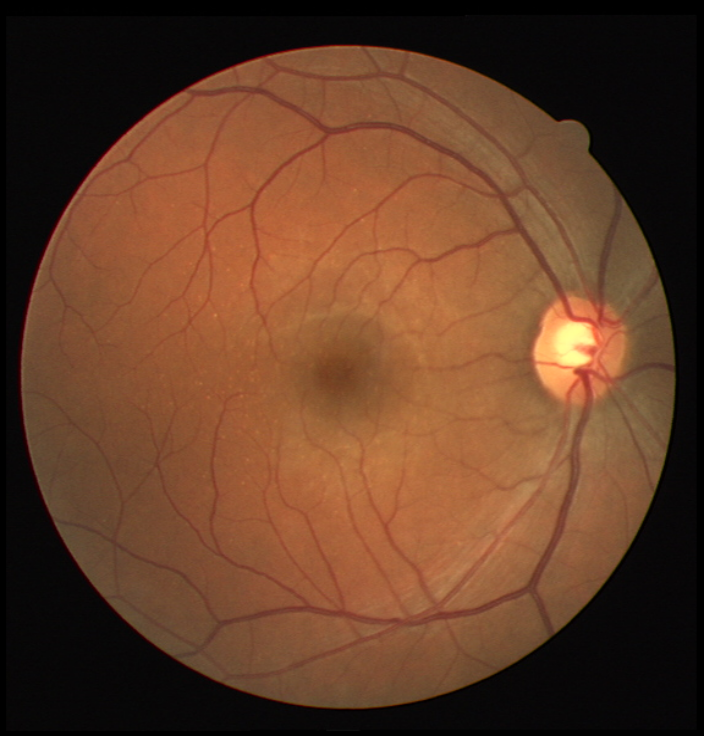
\includegraphics[width=0.8\linewidth]{my_images/contextualizacion/retinografia.jpg}};
			
			% Overlay 2: Disco óptico
			\only<2>{
				\coordinate (retina) at ($(img.south west) + (3.6cm,2.4cm)$);
				\draw[red, thick] (retina) circle (0.35cm);
				\node[red, anchor=north] at ($(retina)+(0,-0.4cm)$) {\footnotesize Disco óptico};
			}
			% Overlay 3: Fóvea
			\only<3>{
				\coordinate (fovea) at ($(img.south west) + (2.1cm,2.2cm)$);
				\draw[red, thick] (fovea) circle (0.25cm);
				\node[red, below] at (fovea) {\footnotesize Fóvea};
			}
			% Overlay 4: Arterias y venas
			\only<4>{
				\coordinate (vena) at ($(img.south west) + (3.5cm,1.5cm)$);
				\draw[red, thick] (vena) circle (0.15cm);
				\node[red, below] at (vena) {\footnotesize Vena};
				
				\coordinate (arteria) at ($(img.south west) + (3.4cm,3.2cm)$);
				\draw[red, thick] (arteria) circle (0.15cm);
				\node[red, below] at (arteria) {\footnotesize Arteria};
			}
			% Overlay 5: Cruces y Bifurcaciones
			\only<5>{
				\coordinate (bifurcacion) at ($(img.south west) + (3.3cm,0.9cm)$);
				\draw[red, thick] (bifurcacion) circle (0.15cm);
				\node[red, below] at (bifurcacion) {\footnotesize Bifurcación};
				
				\coordinate (cruce) at ($(img.south west) + (3.1cm,3.3cm)$);
				\draw[red, thick] (cruce) circle (0.15cm);
				\node[red, below] at (cruce) {\footnotesize Cruce};
			}
			% Overlay 6: Copa y Anillo
			\only<6>{
				\coordinate (copa) at ($(img.south west) + (3.6cm,2.4cm)$);
				\draw[red, thick] (copa) circle (0.35cm);
				\node[red, anchor=north] at ($(copa)+(0,-0.4cm)$) {\footnotesize Copa y Anillo};
			}
		\end{tikzpicture}
	\end{columns}
	
\vspace{-0.5cm}
\begin{center}
	\hspace*{-0.5cm} % Ajusta este valor si es necesario
	
	\uncover<2->{%
		\begin{minipage}[t]{0.1\linewidth}
			\centering
			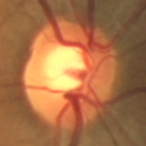
\includegraphics[width=\linewidth]{my_images/contextualizacion/image2.png}\\[0.5ex]
			\footnotesize Disco óptico
		\end{minipage}\hspace{0.5cm}%
	}%
	\uncover<3->{%
		\begin{minipage}[t]{0.1\linewidth}
			\centering
			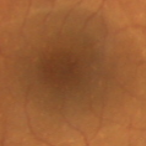
\includegraphics[width=\linewidth]{my_images/contextualizacion/image1.png}\\[0.5ex]
			\footnotesize Fóvea
		\end{minipage}\hspace{0.5cm}%
	}%
	\uncover<4->{%
		\begin{minipage}[t]{0.1\linewidth}
			\centering
			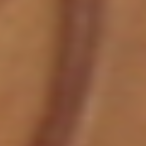
\includegraphics[width=\linewidth]{my_images/contextualizacion/image4.png}\\[0.5ex]
			\footnotesize Venas
		\end{minipage}\hspace{0.5cm}%
		\begin{minipage}[t]{0.1\linewidth}
			\centering
			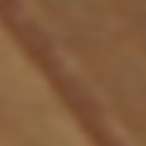
\includegraphics[width=\linewidth]{my_images/contextualizacion/image3.png}\\[0.5ex]
			\footnotesize Arterias
		\end{minipage}\hspace{0.5cm}%
	}%
	\uncover<5->{%
		\begin{minipage}[t]{0.1\linewidth}
			\centering
			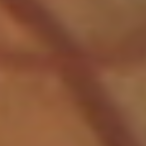
\includegraphics[width=\linewidth]{my_images/contextualizacion/image5.png}\\[0.5ex]
			\footnotesize Cruce
		\end{minipage}\hspace{0.5cm}%
		\begin{minipage}[t]{0.1\linewidth}
			\centering
			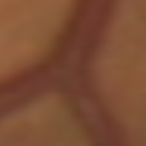
\includegraphics[width=\linewidth]{my_images/contextualizacion/image6.png}\\[0.5ex]
			\footnotesize Bifurcación
		\end{minipage}\hspace{0.5cm}%
	}%
	\uncover<6->{%
		\begin{minipage}[c]{0.1\linewidth}
			\centering
			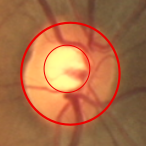
\includegraphics[width=\linewidth]{my_images/contextualizacion/image7.png}\\[0.5ex]
			\footnotesize Anillo y Copa
		\end{minipage}%
	}
\end{center}



\end{frame}



\section{Estado del arte}
% Frame 1: Estracción de estructuras
\begin{frame}{Estado del arte: Estracción de estructuras}
	\begin{columns}[c]
		% Columna izquierda: listado de estructuras
		\column{0.5\textwidth}
		\begin{block}{Segmentación estructuras retinianas}
			\begin{itemize}
				\item Tradicionalmente usando Single Task Learning
				\begin{enumerate}
					\item Mucho gasto computacional.
					\item Falta de transferencia de conocimiento.
				\end{enumerate}
			\end{itemize}
		\end{block}
		
		% Columna derecha: retinografía y anotaciones
		\column{0.5\textwidth}
		\vspace{4cm}
		\centering
		\begin{tikzpicture}[remember picture, overlay]
			% Imágenes centrales: se iteran 5 veces para 5 filas
			\foreach \i in {0,...,4} {
				\node[anchor=center, inner sep=0] at (0,-\i*1.2) {%
					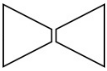
\includegraphics[width=0.2\linewidth]{my_images/curvasROC/red.png}%
				};
			}
			% Imágenes de la izquierda (fuera del for)
			\node[anchor=center, inner sep=0] at (-1.5,0) {%
				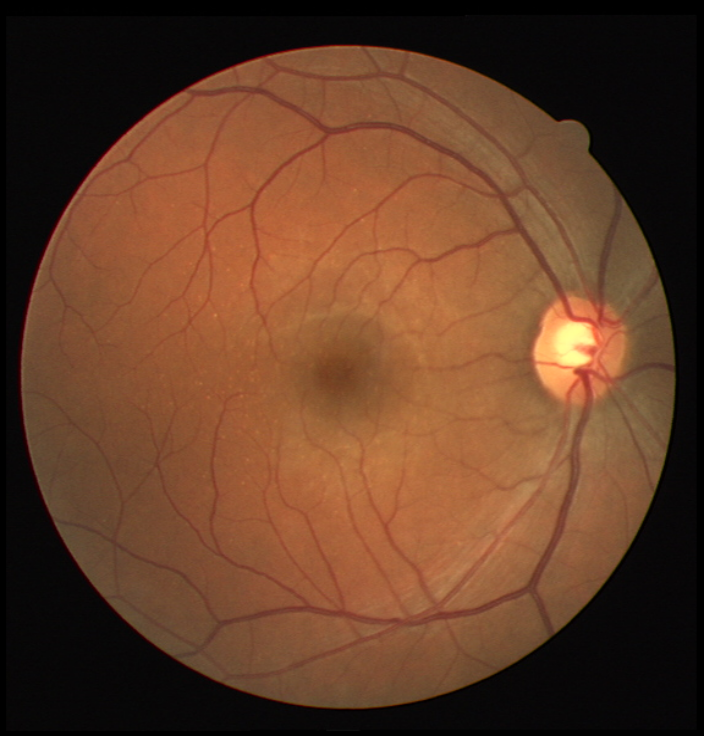
\includegraphics[width=0.2\linewidth]{my_images/ML/36_training.jpg}%
			};
			\node[anchor=center, inner sep=0] at (-1.5,-1.2) {%
				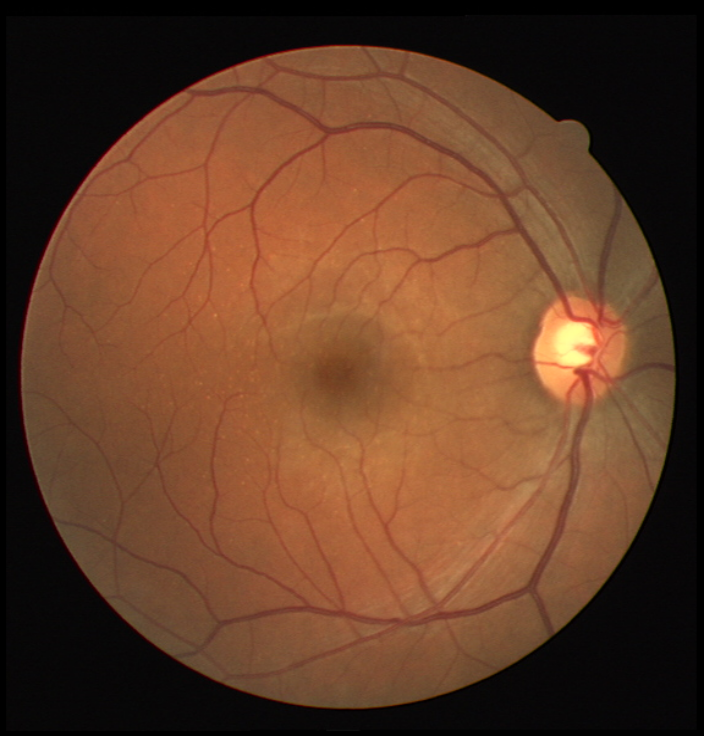
\includegraphics[width=0.2\linewidth]{my_images/ML/36_training.jpg}%
			};
			\node[anchor=center, inner sep=0] at (-1.5,-2.4) {%
				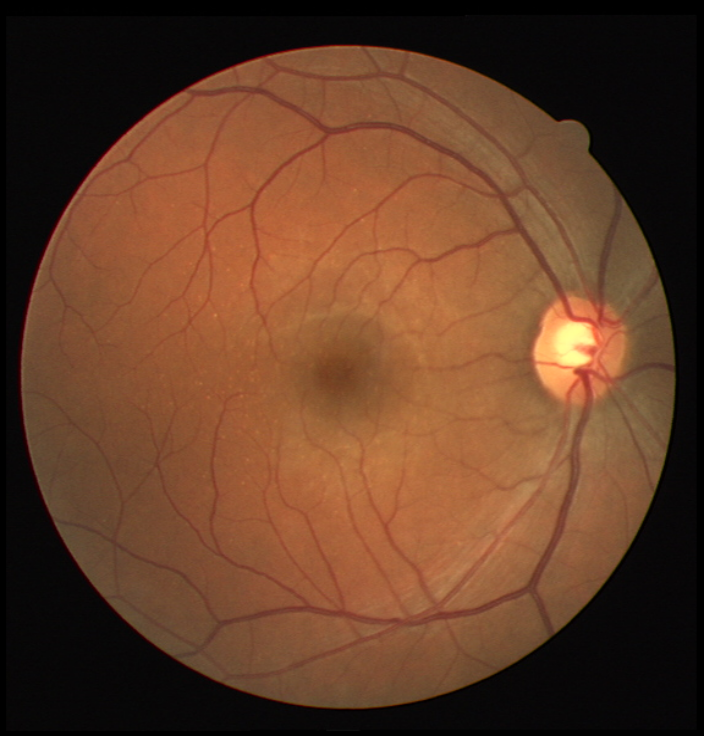
\includegraphics[width=0.2\linewidth]{my_images/ML/36_training.jpg}%
			};
			\node[anchor=center, inner sep=0] at (-1.5,-3.6) {%
				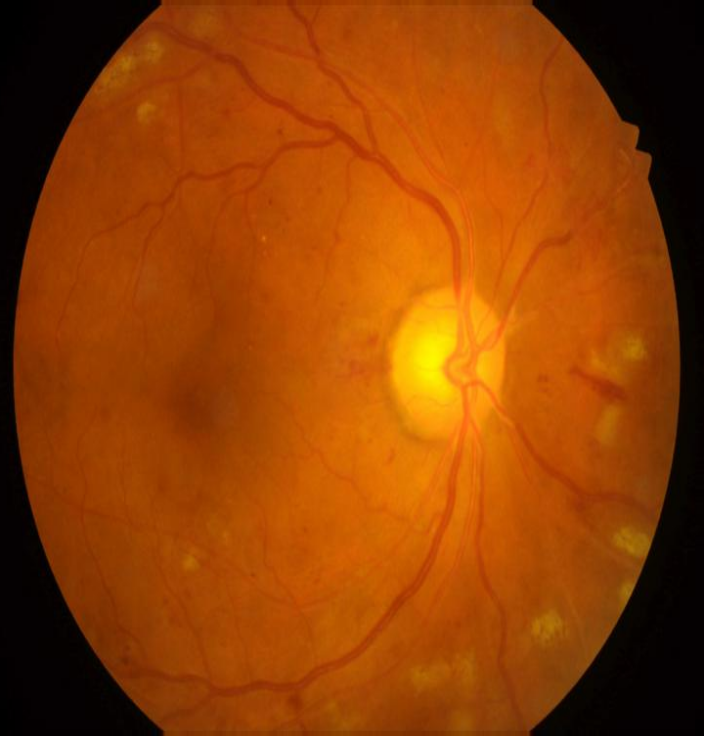
\includegraphics[width=0.2\linewidth]{my_images/ML/IDRiD_010.jpg}%
			};
			\node[anchor=center, inner sep=0] at (-1.5,-4.8) {%
				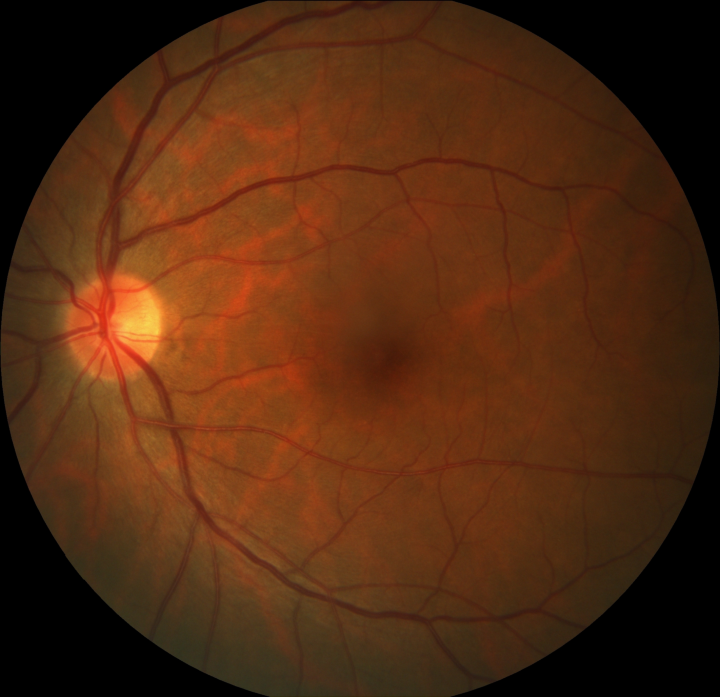
\includegraphics[width=0.2\linewidth]{my_images/ML/n0109.png}%
			};
			% Imágenes de la derecha (fuera del for)
			\node[anchor=center, inner sep=0] at (1.5,0) {%
				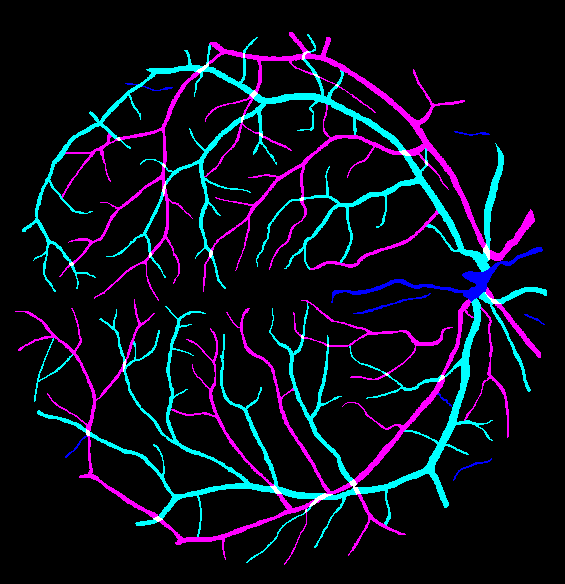
\includegraphics[width=0.2\linewidth]{my_images/ML/36_av.png}%
			};
			\node[anchor=center, inner sep=0] at (1.5,-1.2) {%
				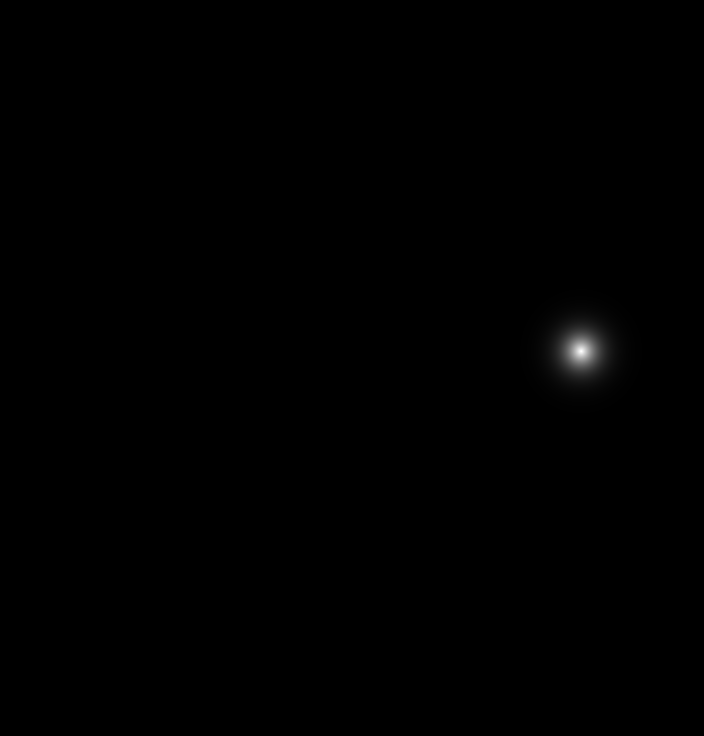
\includegraphics[width=0.2\linewidth]{my_images/ML/OD_36.jpg}%
			};
			\node[anchor=center, inner sep=0] at (1.5,-2.4) {%
				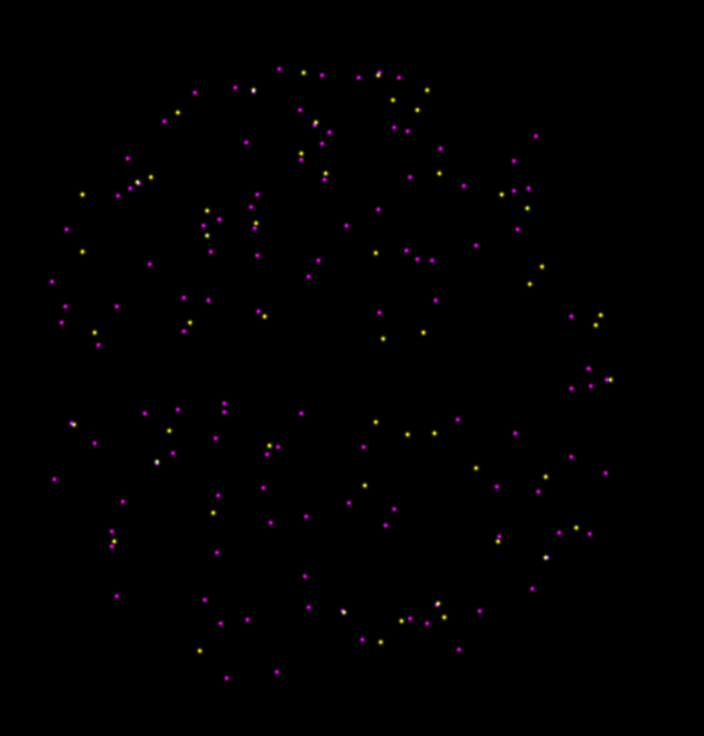
\includegraphics[width=0.2\linewidth]{my_images/ML/jun_36.jpg}%
			};
			\node[anchor=center, inner sep=0] at (1.5,-3.6) {%
				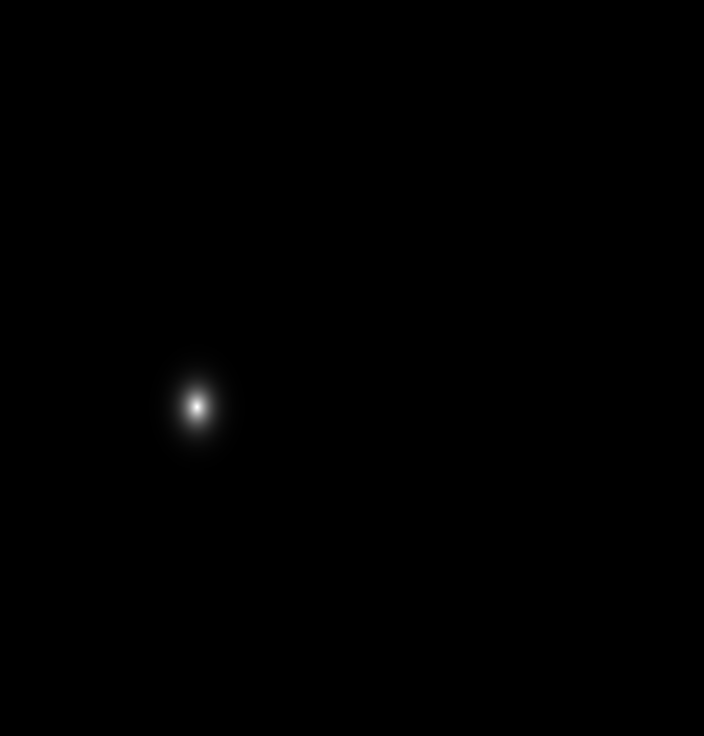
\includegraphics[width=0.2\linewidth]{my_images/ML/fovea_10.jpg}%
			};
			\node[anchor=center, inner sep=0] at (1.5,-4.8) {%
				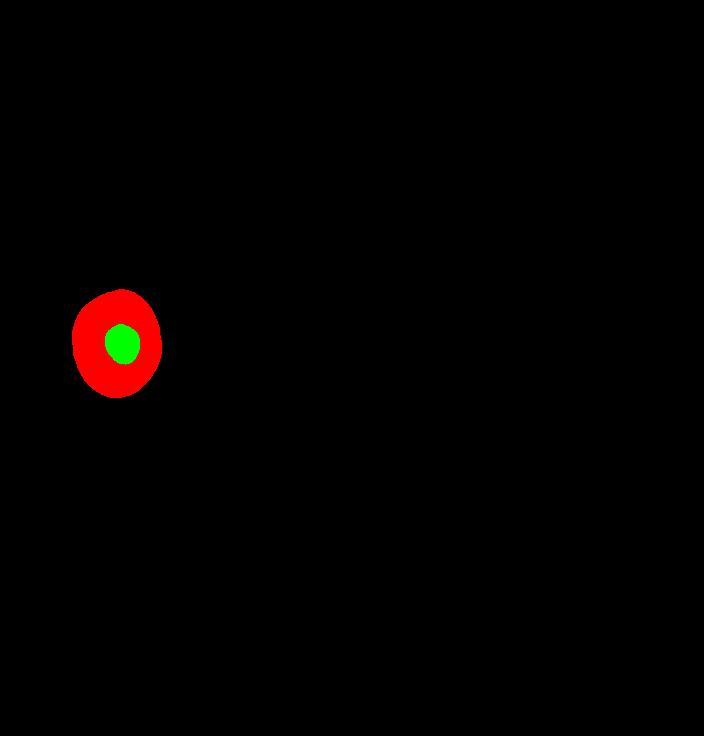
\includegraphics[width=0.2\linewidth]{my_images/ML/hard.jpg}%
			};
		\end{tikzpicture}
	\end{columns}
\end{frame}

% Frame 2: Propuesta
\begin{frame}{Estado del arte: Propuesta}
	\begin{columns}[c]
		% Columna izquierda: Propuesta de Multi Task Learning
		\column{0.5\textwidth}
		\begin{block}{Propuesta}
			\begin{itemize}
				\item Multi Task Learning.
				\item Ventajas teóricas:
				\begin{enumerate}
					\item Compartición de parámetros.
					\item Transferencia de conocimiento.
				\end{enumerate}
				\item Limitaciones:
				\begin{enumerate}
					\item Desbalanceo de tareas.
					\item Interferencia negativa.
				\end{enumerate}
			\end{itemize}
		\end{block}
		
		% Columna derecha: Imágenes organizadas
		\column{0.5\textwidth}
		\vfill
		\vspace{-0.3cm} % Ajusta para posicionar verticalmente
		\begin{columns}[c]
			% Subcolumna izquierda: Una imagen
			\column{0.3\linewidth}
			\begin{center}
				\hspace*{0.4cm}
				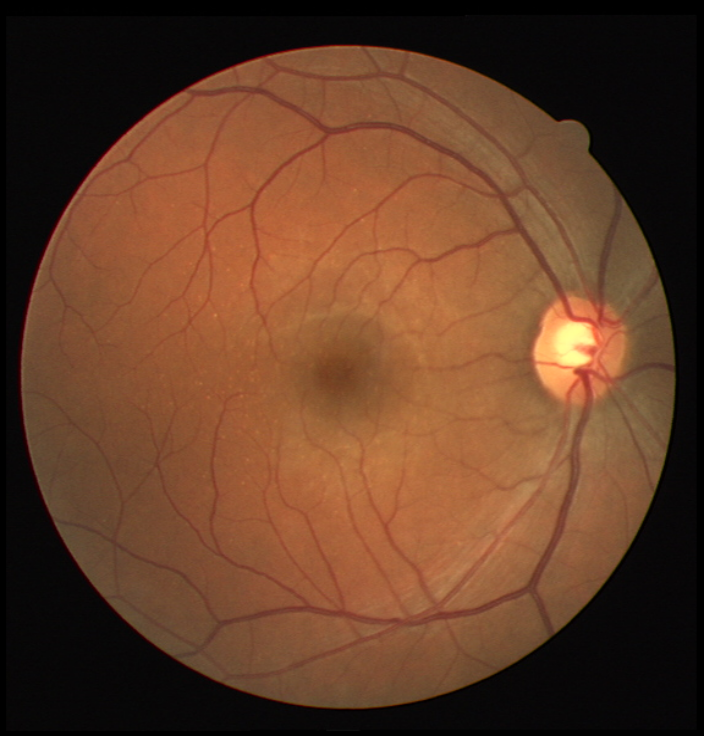
\includegraphics[width=\linewidth]{my_images/ML/36_training.jpg}
			\end{center}
			% Subcolumna central: Imagen central
			\column{0.3\linewidth}
			\begin{center}
				\hspace*{0.4cm}
				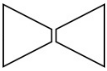
\includegraphics[width=\linewidth]{my_images/curvasROC/red.png}
			\end{center}
			% Subcolumna derecha: Cinco imágenes apiladas
			\column{0.4\linewidth}
			\begin{center}
				\vspace*{0.4cm}
				\hspace*{-0.2cm}
				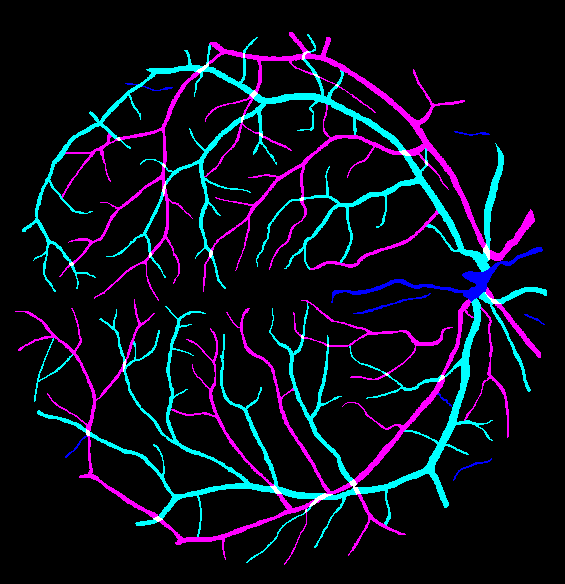
\includegraphics[width=0.5\linewidth]{my_images/ML/36_av.png}\\[0.2cm]
				\hspace*{-0.2cm}
				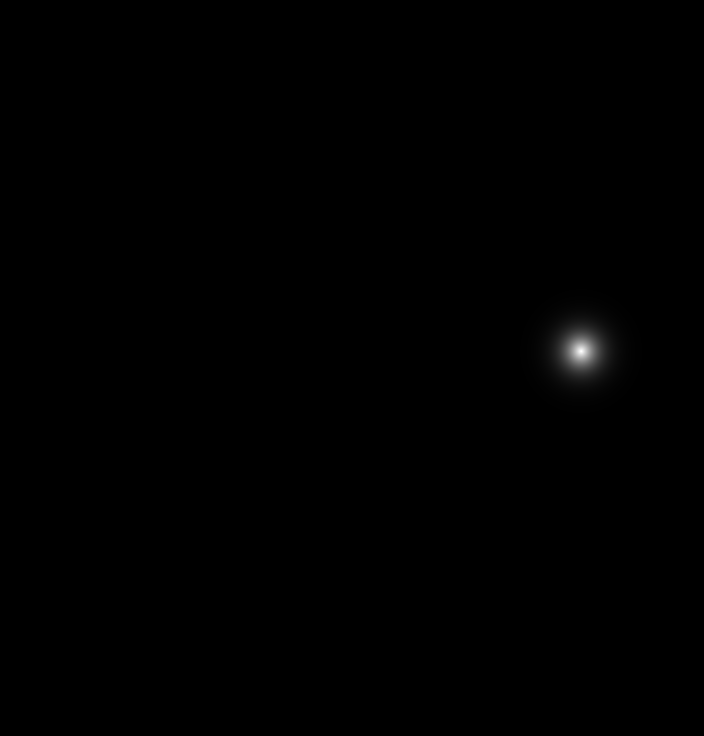
\includegraphics[width=0.5\linewidth]{my_images/ML/OD_36.jpg}\\[0.2cm]
				\hspace*{-0.2cm}
				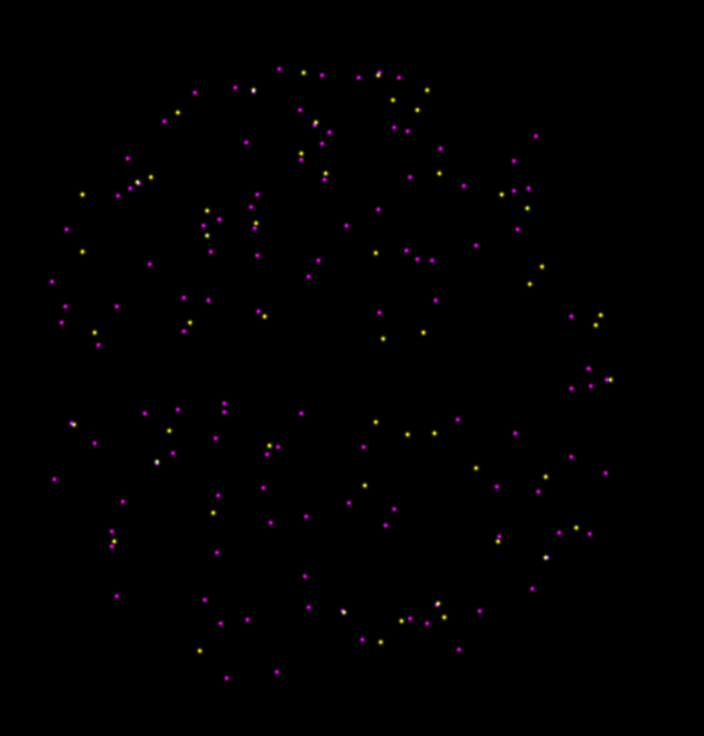
\includegraphics[width=0.5\linewidth]{my_images/ML/jun_36.jpg}\\[0.2cm]
				\hspace*{-0.2cm}
				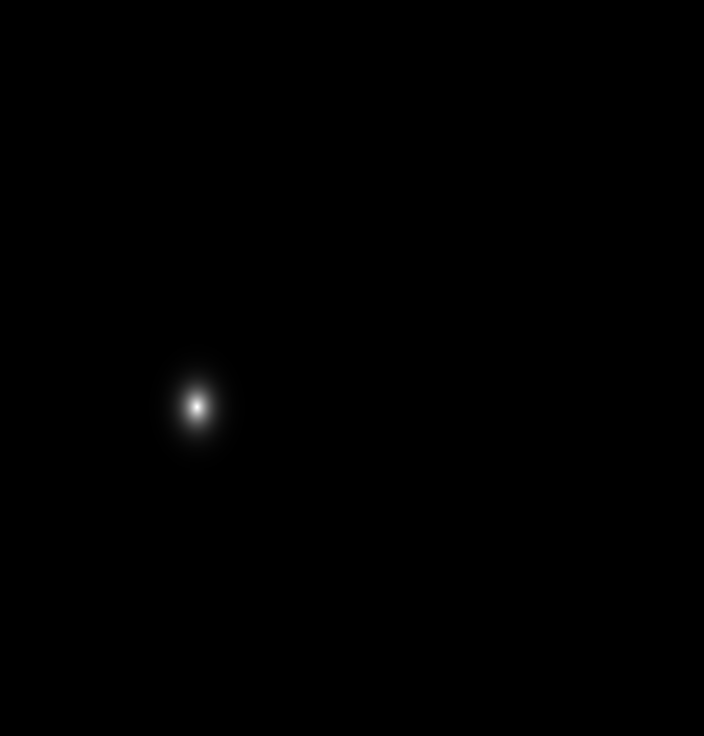
\includegraphics[width=0.5\linewidth]{my_images/ML/fovea_10.jpg}\\[0.2cm]
				\hspace*{-0.2cm}
				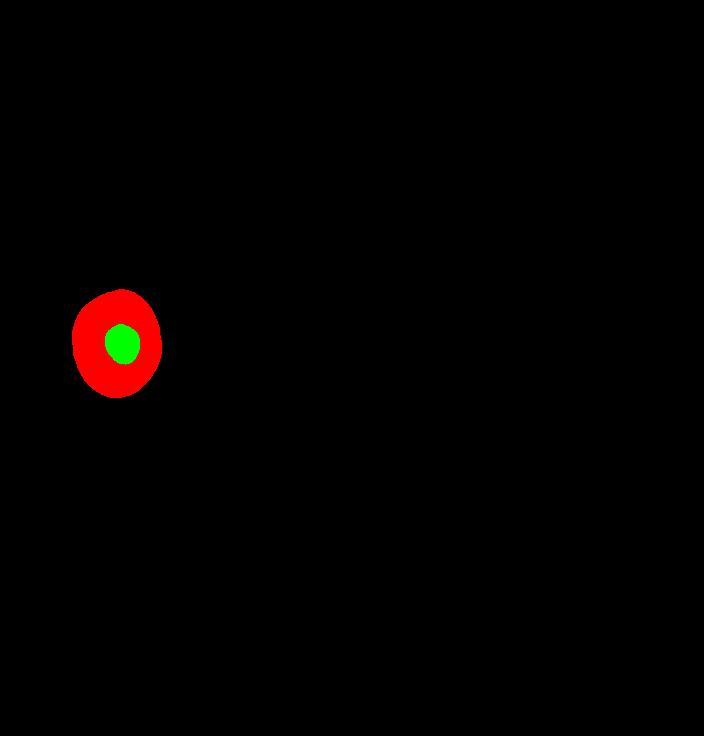
\includegraphics[width=0.5\linewidth]{my_images/ML/hard.jpg}
			\end{center}
		\end{columns}
		\vfill
	\end{columns}
\end{frame}

\begin{frame}{Estado del arte: Propuesta}
	\begin{block}{Posibles soluciones al desbalanceo de tareas.}
		\begin{itemize}
			\item Ponderación de losses.
							\begin{itemize}
								\item Tedioso.
							\end{itemize}
			\item Uso de arquitecturas especializadas.
			\item Algoritmos basados en optimización adaptativa.
			\begin{enumerate}
				\item DWA
				\item GradNorm
				\item MAO
			\end{enumerate}
		\end{itemize}	
	\end{block}
\end{frame}
% Frame 3: Optimización Multi-Adaptativa
\begin{frame}{Estado del arte: Optimización Multi-Adaptativa}
\scalebox{0.9}{%
	\begin{minipage}{\linewidth}
		\begin{block}{MAO}
			\begin{itemize}
				\item Basado en algoritmos de optimización adaptativa (ADAM)
				\begin{itemize}
					\item Adaptan la tasa de aprendizaje de los parámetros del modelo.
				\end{itemize}
				\item MAO generaliza esta idea a multitarea
				\begin{itemize}
					\item Adapta la tasa de aprendizaje de cada parámetro de forma independiente para cada tarea.
					\item Balancea implícitamente la contribución de cada tarea.
				\end{itemize}
			\end{itemize}
		\end{block}
	\end{minipage}%
}



\begin{center}
	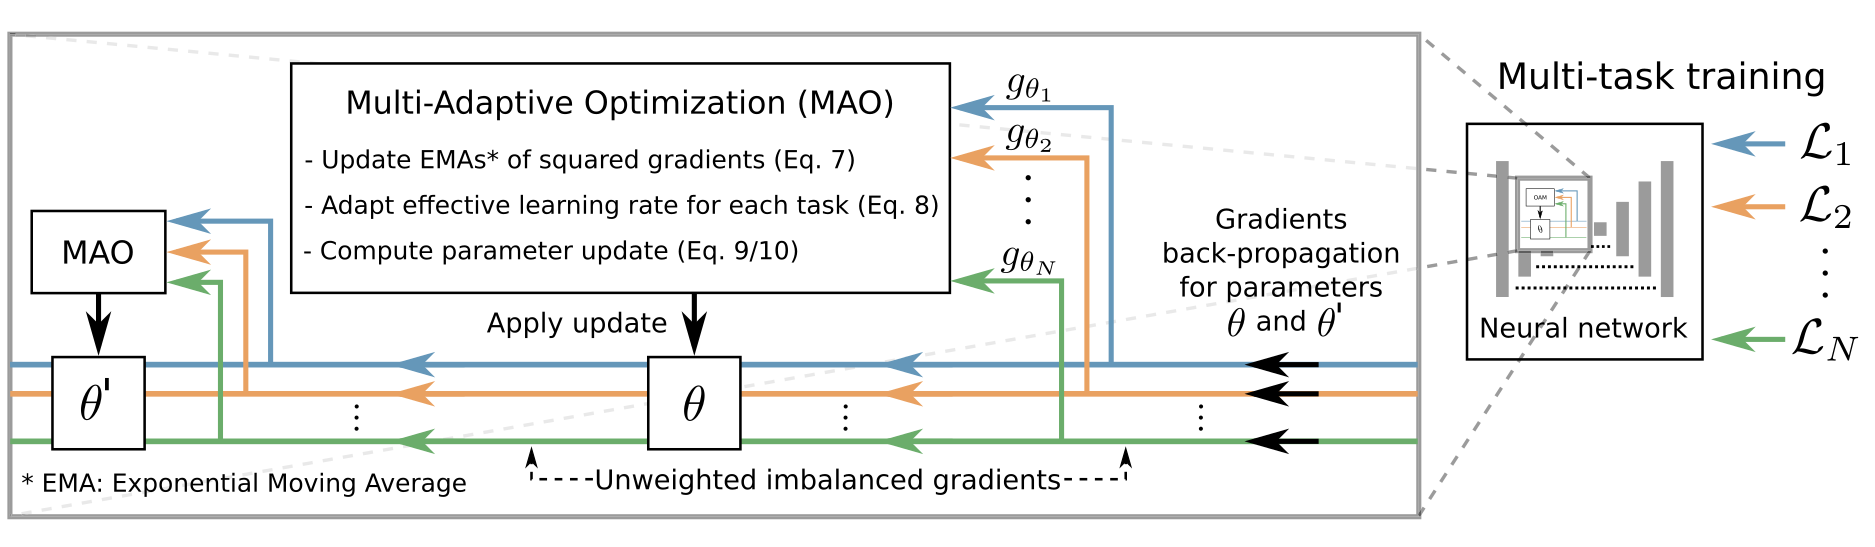
\includegraphics[width=\linewidth]{my_images/ML/mao.png}
\end{center}

\end{frame}


\section{Trabajo Desarrollado}

\begin{frame}{Trabajo Desarrollado: Índice}
	\begin{block}{}
	\begin{enumerate}
		\item Single Task Learning
				\begin{enumerate}
					\item Disco Óptico y Fóvea
					\item Cruces y Bifurcaciones
					\item Segmentación de Arterias y Venas
					\item Segmentación Anillo y Copa del Disco Óptico
				\end{enumerate}
		\item Multi Task Learning
		\item Arquitecturas
	\end{enumerate}
	\end{block}
\end{frame}

\begin{frame}{Trabajo Desarrollado: STL}
	\begin{columns}[T]

		\column{0.5\textwidth}
		
		\begin{block}{Detección Disco Óptico y Fóvea}
			\begin{itemize}
				\item Objetivos:
				\begin{enumerate}
					\item Localizar Disco Óptico
					\item Localizar Fóvea
				\end{enumerate}
				\item Se conoce el centro de la estructura.
						\begin{itemize}
							\item Mapa binario.
							\item Se transforma en un mapa de calor.
						\end{itemize}

				\item MSE.
			\end{itemize}
		\end{block}
 \column{0.5\textwidth}
% Primera fila: dos imágenes en paralelo
\begin{minipage}[t]{0.35\textwidth}
	\centering
	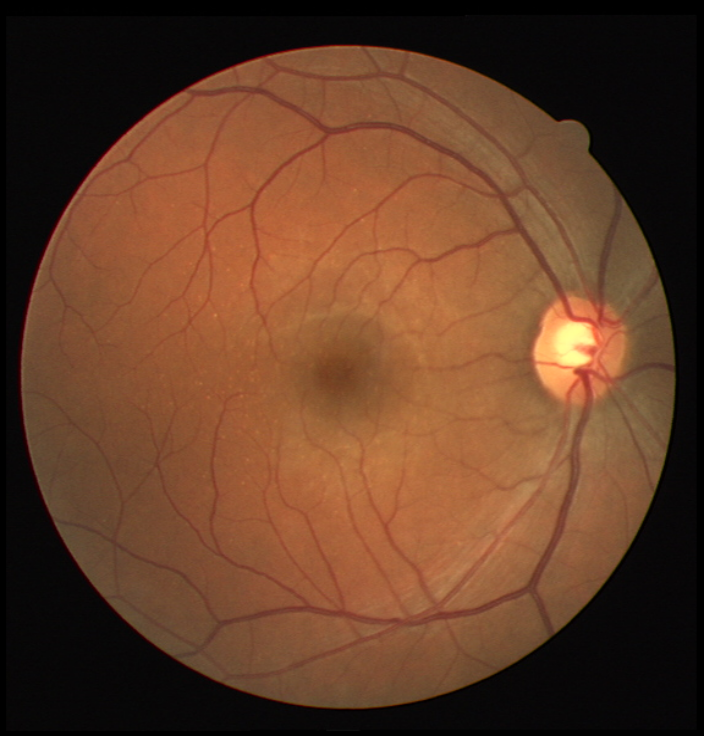
\includegraphics[width=\textwidth]{my_images/ML/36_training.jpg}\\[1ex]
	{\small Retinografía}
\end{minipage}\hfill
\begin{minipage}[t]{0.35\textwidth}
	\centering
	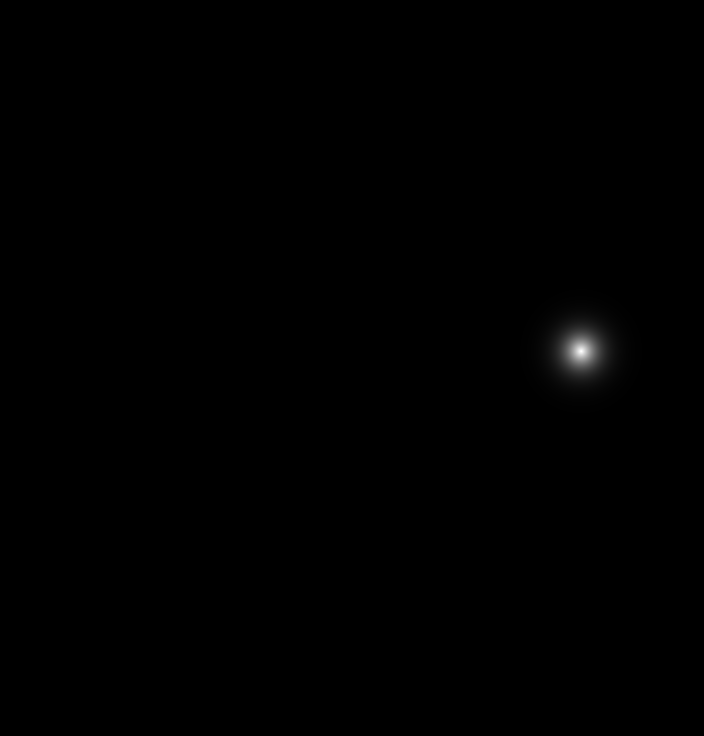
\includegraphics[width=\textwidth]{my_images/ML/OD_36.jpg}\\[1ex]
	{\small \mbox{Disco Óptico}}
\end{minipage}

\vspace{1em} % Espacio entre filas

% Segunda fila: dos imágenes en paralelo
\begin{minipage}[t]{0.35\textwidth}
	\centering
	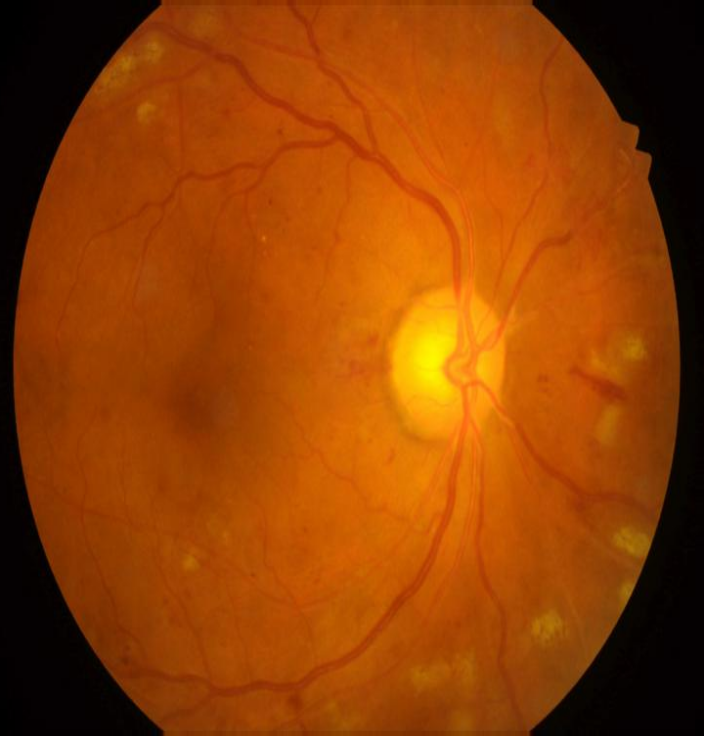
\includegraphics[width=\textwidth]{my_images/ML/IDRiD_010.jpg}\\[1ex]
	{\small Retinografía}
\end{minipage}\hfill
\begin{minipage}[t]{0.35\textwidth}
	\centering
	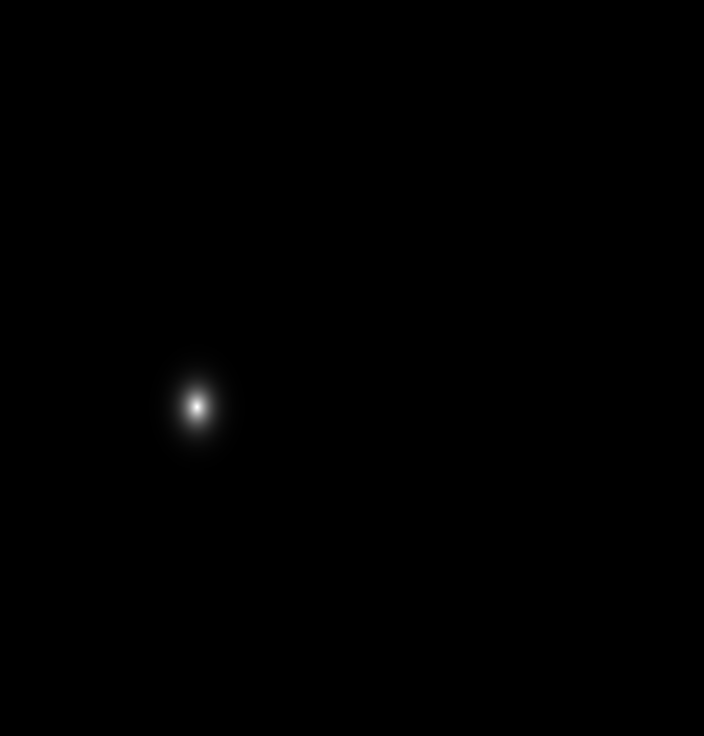
\includegraphics[width=\textwidth]{my_images/ML/fovea_10.jpg}\\[1ex]
	{\small Fóvea}
\end{minipage}
\end{columns}
\end{frame}

\begin{frame}{Trabajo Desarrollado: STL }
	\begin{columns}[T]
	\column{0.5\textwidth}
	\vspace{-0.6cm}
  \scalebox{0.9}{%
	\begin{minipage}{\linewidth}
		\begin{block}{Detección de Cruces y Bifurcaciones}
			\begin{itemize}
				\item Objetivos.
				\begin{enumerate}
					\item Localizar los puntos.
					\item Distinguir entre Cruces y Bifurcaciones.
				\end{enumerate}
				\item Se conoce la localización de los puntos.
				\item Un canal para cruces, un canal para bifurcaciones y un canal para el conjunto de cruces y bifurcaciones.
				\begin{itemize}
					\item Se transforman los mapas binarios en mapas de calor.
				\end{itemize}
				\item 3 MSE.
			\end{itemize}
		\end{block}
	\end{minipage}
}
	\column{0.5\textwidth}
	\begin{center}
		\begin{minipage}[t]{0.5\textwidth}
			\centering
			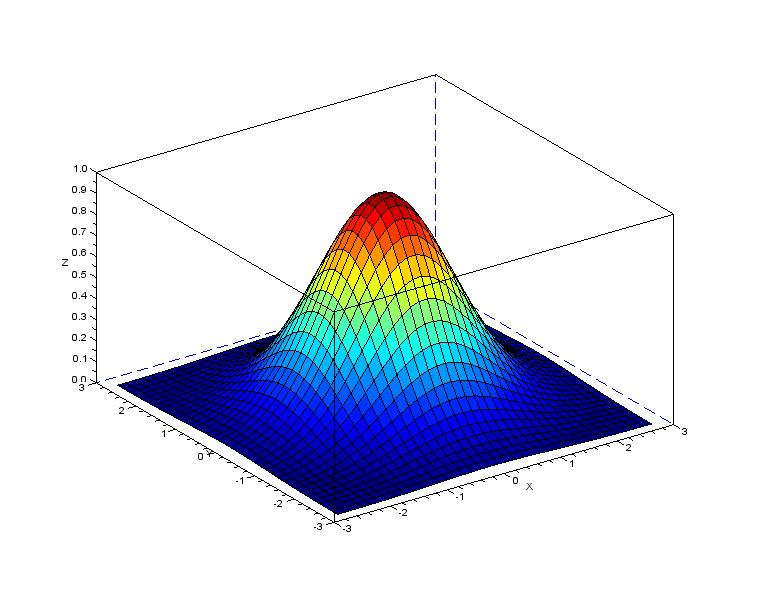
\includegraphics[width=\textwidth]{my_images/ML/gaussiankernel.jpg}
					{\small \mbox{Kernel Gaussiano}}
		\end{minipage}
	\end{center}
	
	% Espacio entre filas
	
	% Segunda fila: dos imágenes en paralelo
	\begin{minipage}[t]{0.35\textwidth}
		\centering
		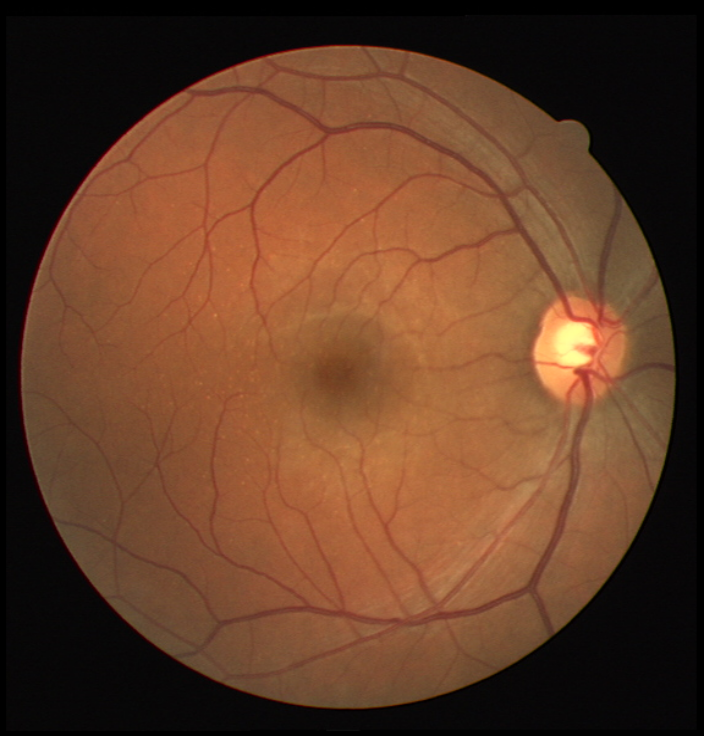
\includegraphics[width=\textwidth]{my_images/ML/36_training.jpg}\\[1ex]
		{\small Retinografía}
	\end{minipage}\hfill
	\begin{minipage}[t]{0.35\textwidth}
		\centering
		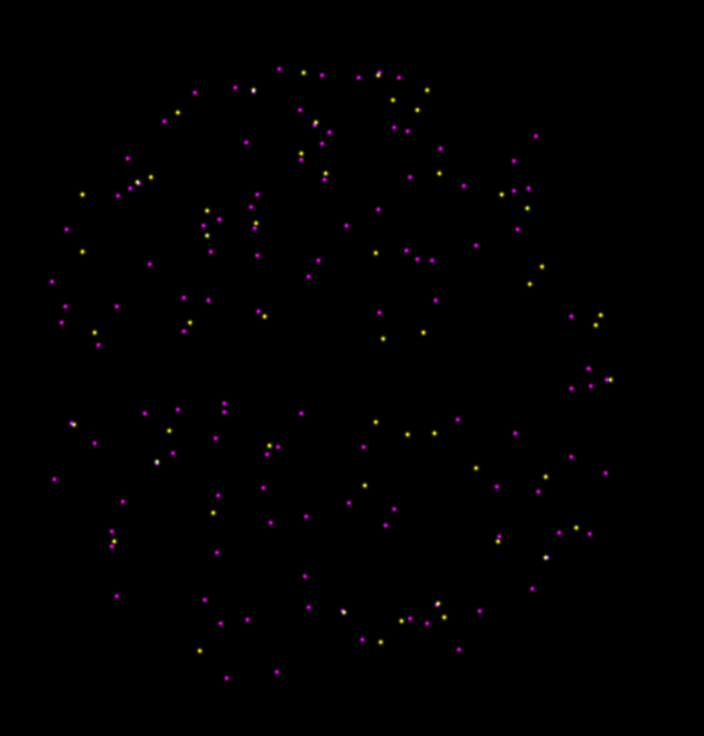
\includegraphics[width=\textwidth]{my_images/ML/jun_36.jpg}\\[1ex]
		{\small \mbox{Disco Óptico}}
	\end{minipage}
\end{columns}
\end{frame}


\begin{frame}{Trabajo Desarrollado: STL}
	\begin{columns}[T]
		\column{0.5\textwidth}
		\vspace{0.5cm} % Baja el contenido de la primera columna 0.5 cm
				\vspace{-0.9cm}
		\begin{block}{Segmentación de arterias y venas.}
			\begin{itemize}
				\item Objetivos.
				\begin{enumerate}
					\item Segmentar el árbol vascular.
					\item Distinguir entre Arterias y Venas.
				\end{enumerate}
				\item Se divide el problema en tres tareas:
				\begin{itemize}
					\item Arterias vs fondo.
					\item Venas vs fondo.
					\item Árbol Vascular vs fondo.
				\end{itemize}
				\item Multisegmentación.
				\item 3 BCE.
			\end{itemize}
		\end{block}
		\column{0.5\textwidth}
		\vspace{2cm} % Baja el contenido de la segunda columna 5 cm
		\begin{minipage}[t]{1.2\textwidth}
			\centering
			\hspace{-1.1cm}
			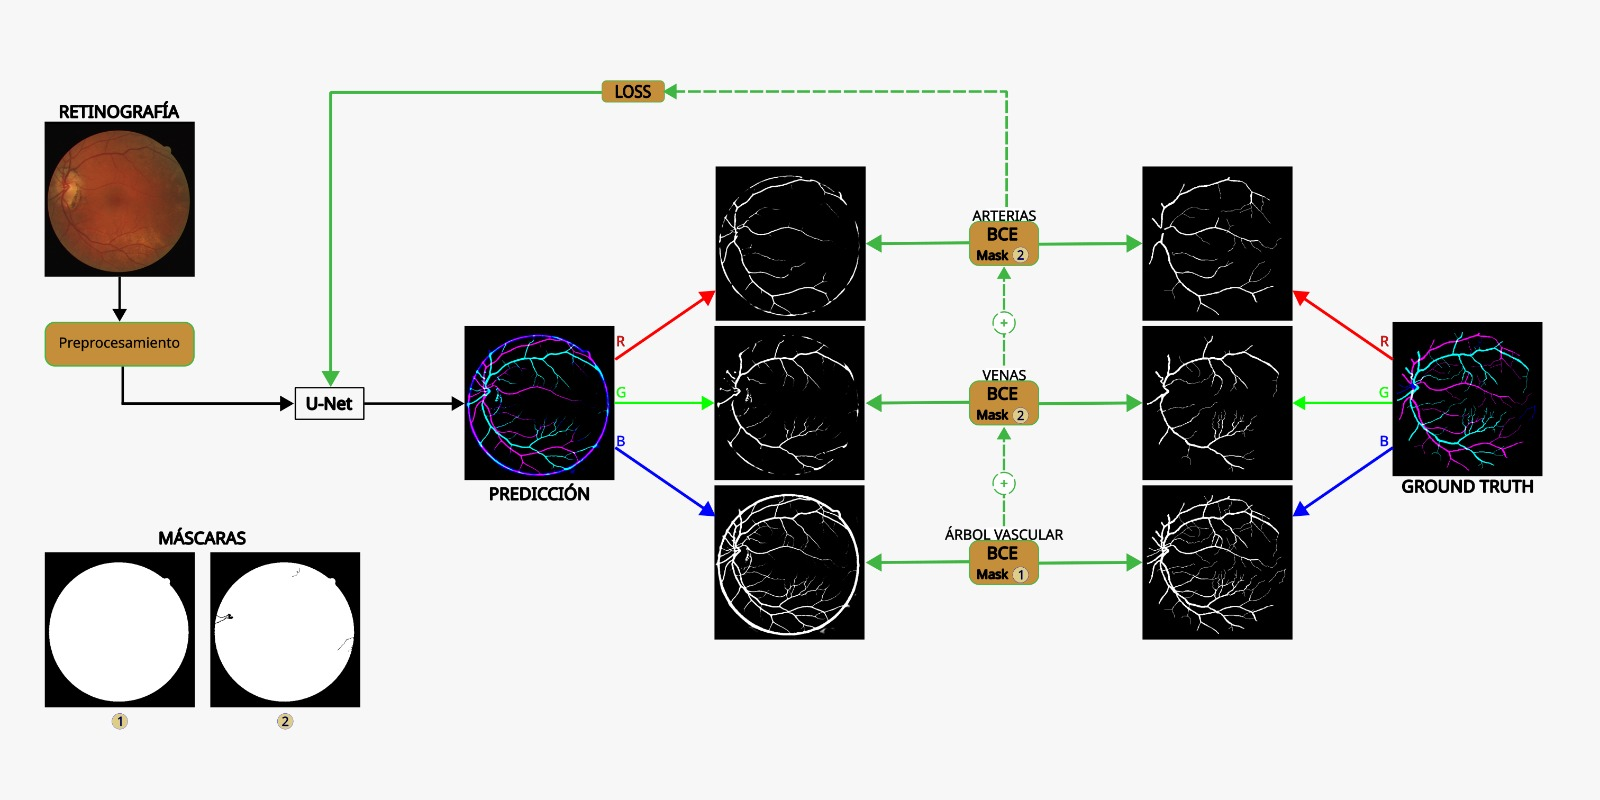
\includegraphics[width=\textwidth]{my_images/ML/AV.jpg}
		\end{minipage}
	\end{columns}
\end{frame}


\begin{frame}{Trabajo Desarrollado: STL}
	\begin{columns}[T]
		\column{0.5\textwidth}
		\vspace{-0.5cm} % Baja el contenido de la primera columna 0.5 cm
		\begin{block}{Segmentación de Copa y Anillo del disco óptico}
			\begin{itemize}
				\item Objetivos:
					\begin{itemize}
						\item Segmentar Copa del Disco Óptico.
						\item Segmentar Anillo del Disco Óptico.
					\end{itemize}
					\item Se divide el problema en 3 clases:
					\begin{itemize}
						\item Copa óptica.
						\item Anillo copa óptica.
						\item Fondo.
					\end{itemize}
					\item Segmentación multiclase.
				\item MCE.
			\end{itemize}
		\end{block}
	 \column{0.5\textwidth}
	% Primera fila: dos imágenes en paralelo
	\begin{minipage}[t]{0.35\textwidth}
		\centering
		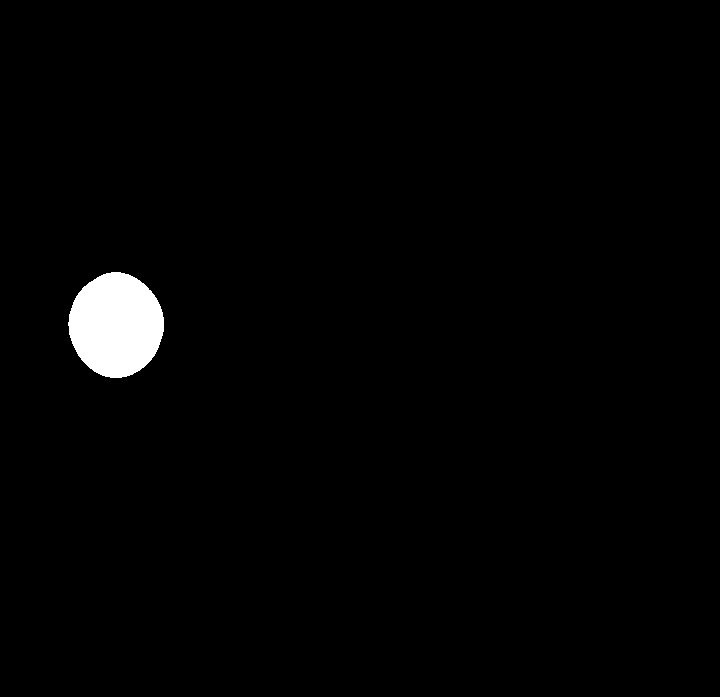
\includegraphics[width=\textwidth]{my_images/ML/n0109_disc.png}\\[1ex]
		{\small Disco óptico}
	\end{minipage}\hfill
	\begin{minipage}[t]{0.35\textwidth}
		\centering
		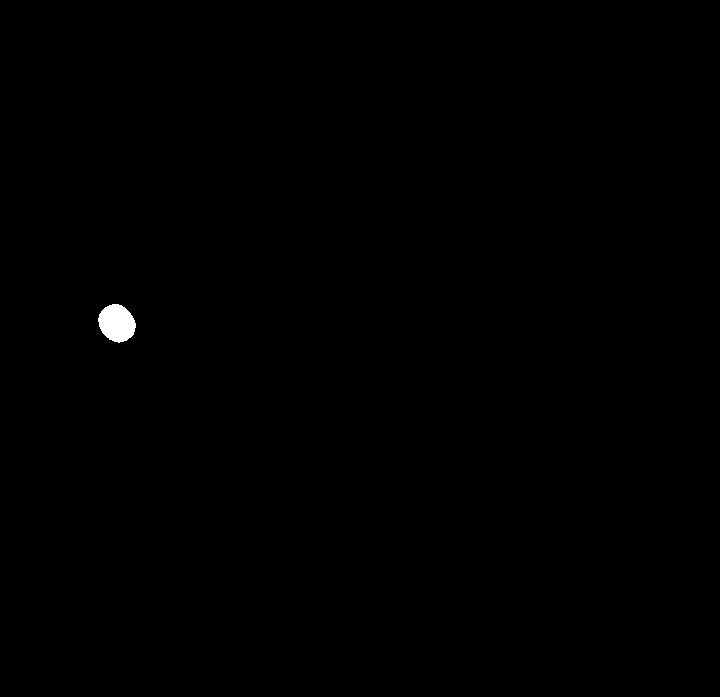
\includegraphics[width=\textwidth]{my_images/ML/n0109_cup.png}\\[1ex]
		{\small \mbox{Copa}}
	\end{minipage}
	
	\vspace{1em} % Espacio entre filas
	
	% Segunda fila: dos imágenes en paralelo
		\centering
	\begin{minipage}[t]{0.35\textwidth}
	
		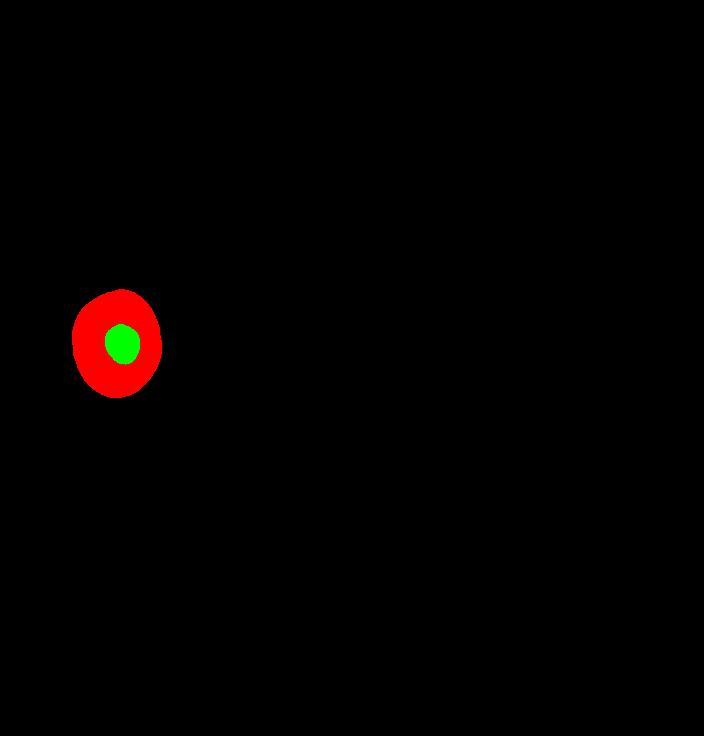
\includegraphics[width=\textwidth]{my_images/ML/hard.jpg}\\[1ex]
		{\small Copa y Anillo}
	\end{minipage}\hfill

	\end{columns}
\end{frame}

\begin{frame}{Trabajo Desarrollado: MTL}
	% Parte superior: bloque principal (aparece en el primer overlay)
	\begin{block}<1->{}
		\begin{itemize}
			\item Entrenar un modelo para las 5 tareas.
			\item 11 canales de salida.
			\item Mismas funciones de pérdida que las tareas originales.
		\end{itemize}
	\end{block}
	
	\vspace{-0.5cm}
	
	% Parte inferior: dos columnas con bloque e imagen en cada una
	\begin{columns}[T,onlytextwidth]
		\column{0.4\textwidth}
		\begin{block}<2->{Baseline}
			Las pérdidas se suman.
			\begin{itemize}
				\item No se balancean.
			\end{itemize}
			
		\end{block}
		\centering
		\only<2->{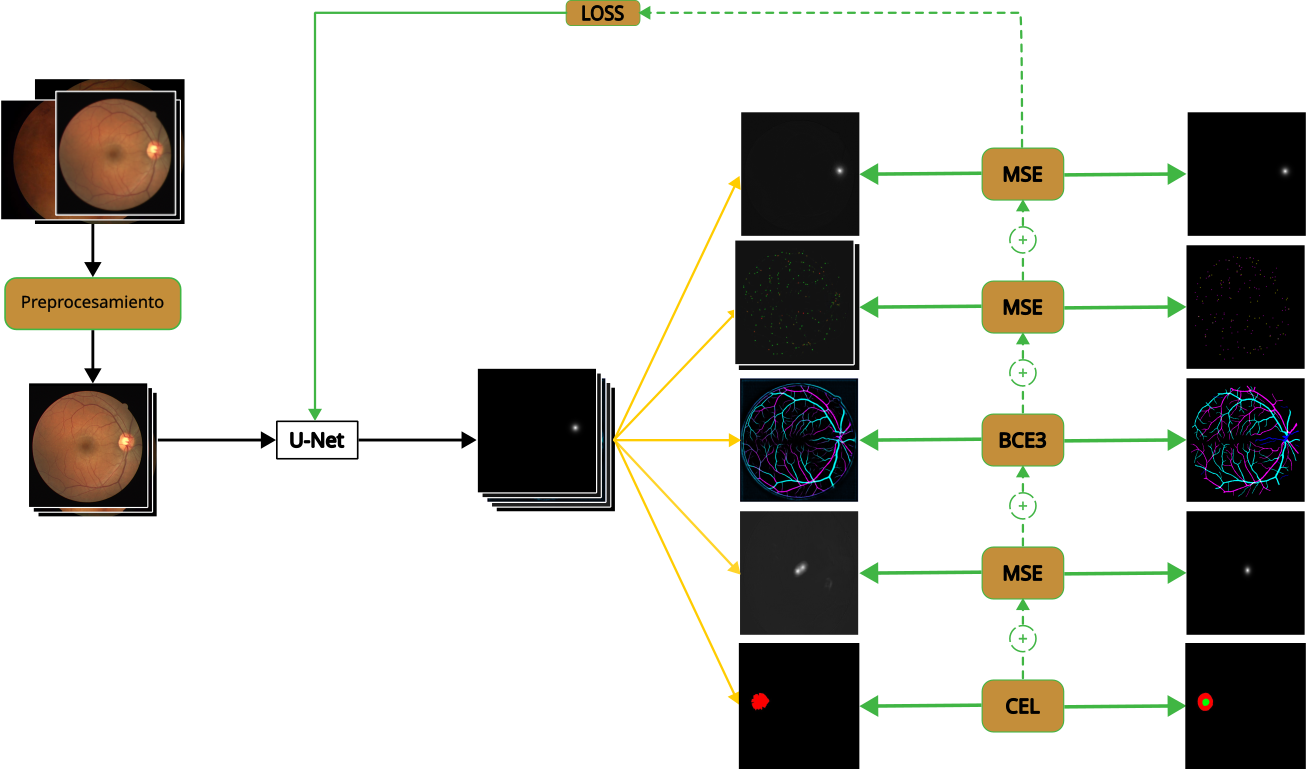
\includegraphics[width=\textwidth]{my_images/ML/MTL.png}\\[1ex]}
		
		\column{0.4\textwidth}
		\begin{block}<3->{MAO}
			Las pérdidas entran al MAO.
		\end{block}
		\centering
		\only<3->{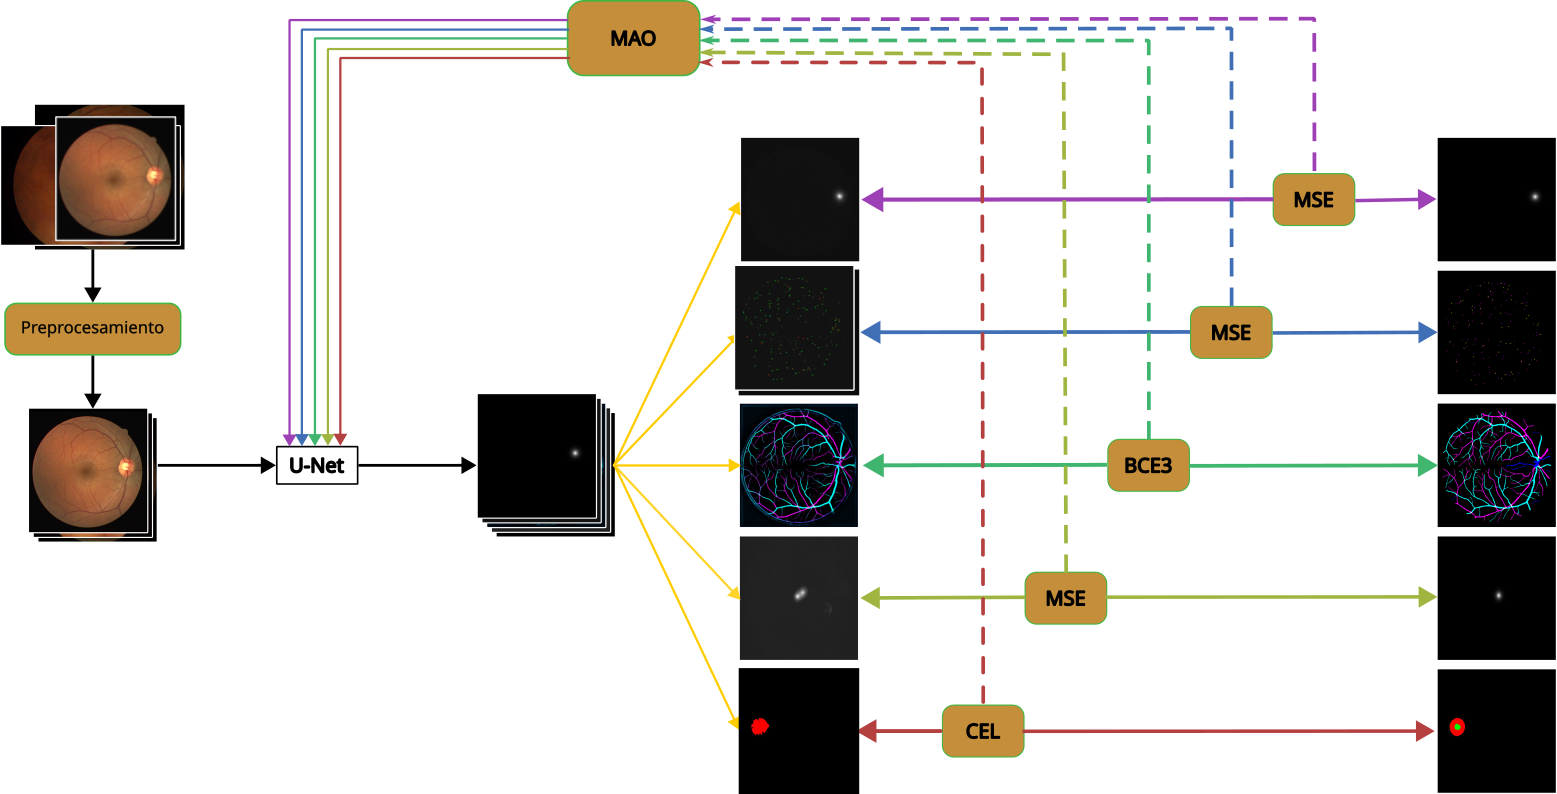
\includegraphics[width=\textwidth]{my_images/ML/g5.png}\\[1ex]}
	\end{columns}
\end{frame}
\begin{comment}


\begin{frame}{Trabajo Desarrollado}
	\begin{columns}[T]
		\column{0.5\textwidth}
		\vspace{0.5cm} % Baja el contenido de la primera columna 0.5 cm
		\begin{block}{Multi Task-Learning}
			\begin{itemize}
				\item Se combinan las diferentes tareas.
				\item 11 canales de salida.
				\item Suma de los diferentes losses.
			\end{itemize}
		\end{block}

		\column{0.5\textwidth}
		% Primera fila: dos imágenes en paralelo
				\vspace{1cm} 
		\begin{minipage}[t]{\textwidth}
			\centering
			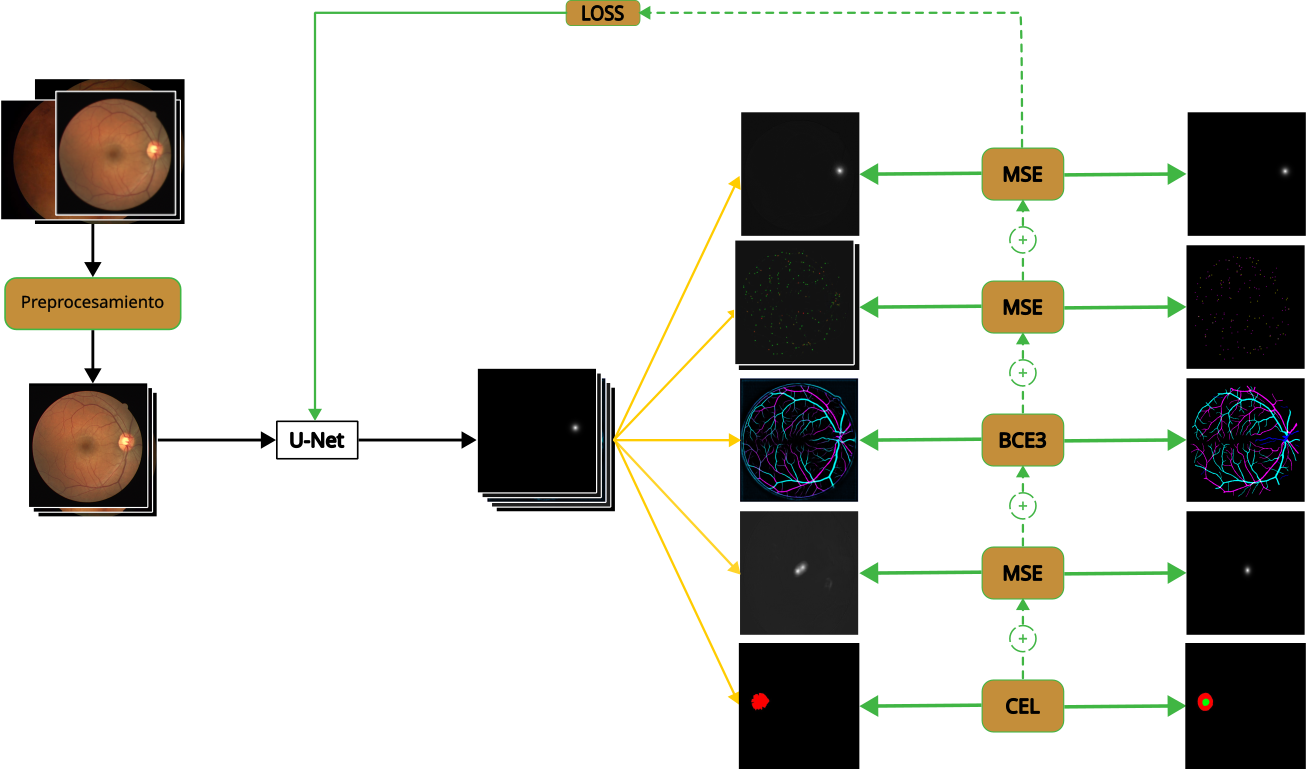
\includegraphics[width=\textwidth]{my_images/ML/MTL.png}\\[1ex]
		\end{minipage}\hfill
	
	\end{columns}
\end{frame}


\begin{frame}{Trabajo Desarrollado}
	\begin{columns}[T]
		\column{0.5\textwidth}
		\vspace{0.5cm} % Baja el contenido de la primera columna 0.5 cm
		\begin{block}{Multi-Adaptative Optimization}
			\begin{itemize}
				\item Se combinan las diferentes tareas.
				\item 11 canales de salida.
				\item Las perdidas entran por separado en MAO.
			\end{itemize}
		\end{block}
		
		\column{0.5\textwidth}
		% Primera fila: dos imágenes en paralelo
		\vspace{1cm} 
		\begin{minipage}[t]{\textwidth}
			\centering
			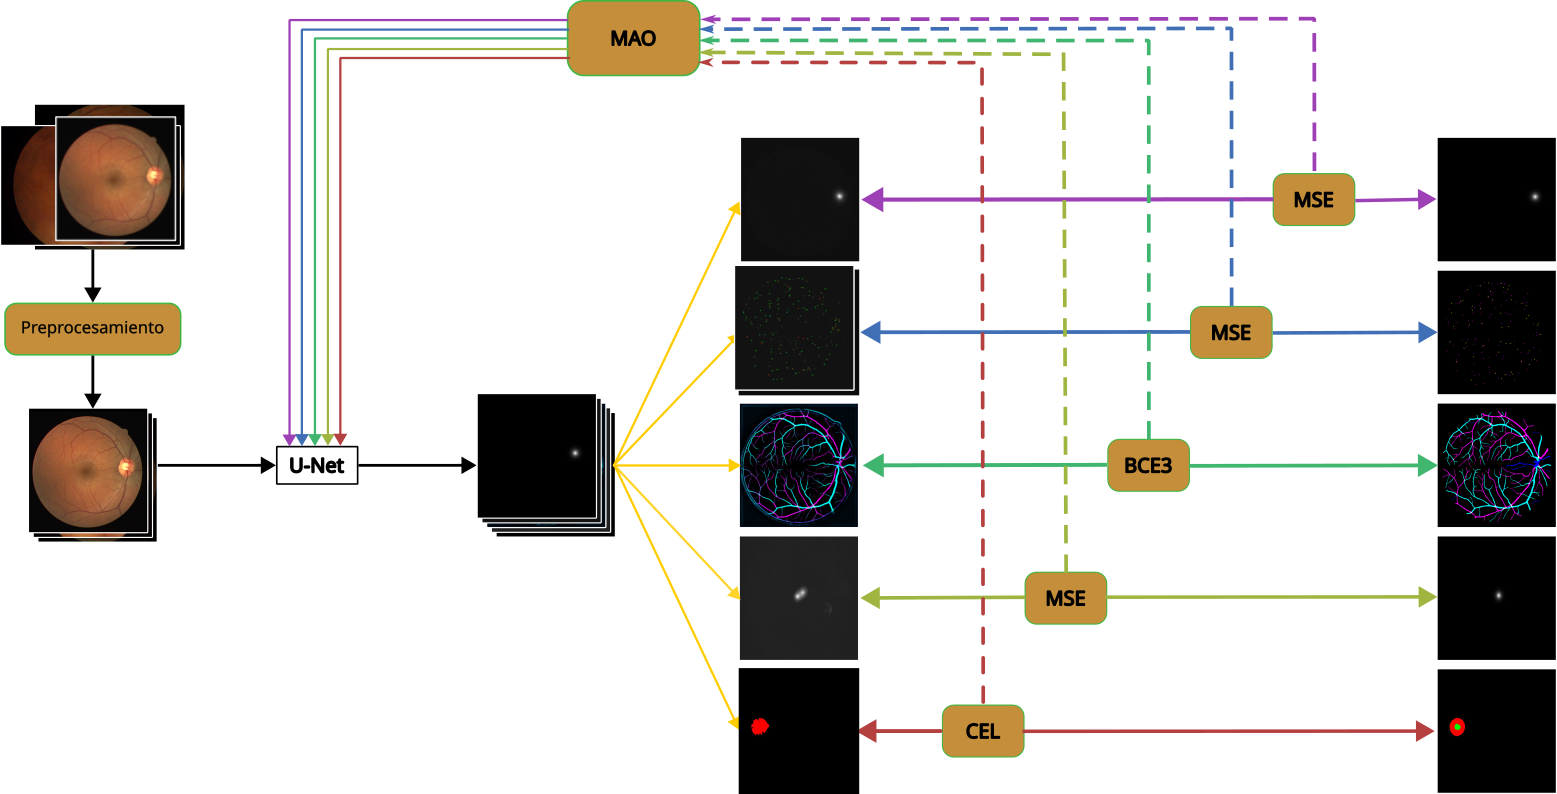
\includegraphics[width=\textwidth]{my_images/ML/g5.png}\\[1ex]
		\end{minipage}\hfill
		
	\end{columns}
\end{frame}
\end{comment}
\begin{frame}{Trabajo Desarrollado: Arquitecturas}
	\begin{columns}[T]
		\column{0.5\textwidth}
		\vspace{0.5cm} % Baja el contenido de la primera columna 0.5 cm
		\begin{block}{U-Net}
			\begin{itemize}
				\item Muy utilizada en computer vision, especialmente en imagen médica.
				\item FCN.
				\item Características:
				\begin{itemize}
					\item Etapa codificadora.
					\item Etapa decodificadora.
					\item Conexiones intermedias.
				\end{itemize}
			\end{itemize}
		\end{block}
		
		\column{0.5\textwidth}
		% Primera fila: dos imágenes en paralelo
		\vspace{1cm} 
		\begin{minipage}[t]{\textwidth}
			\centering
			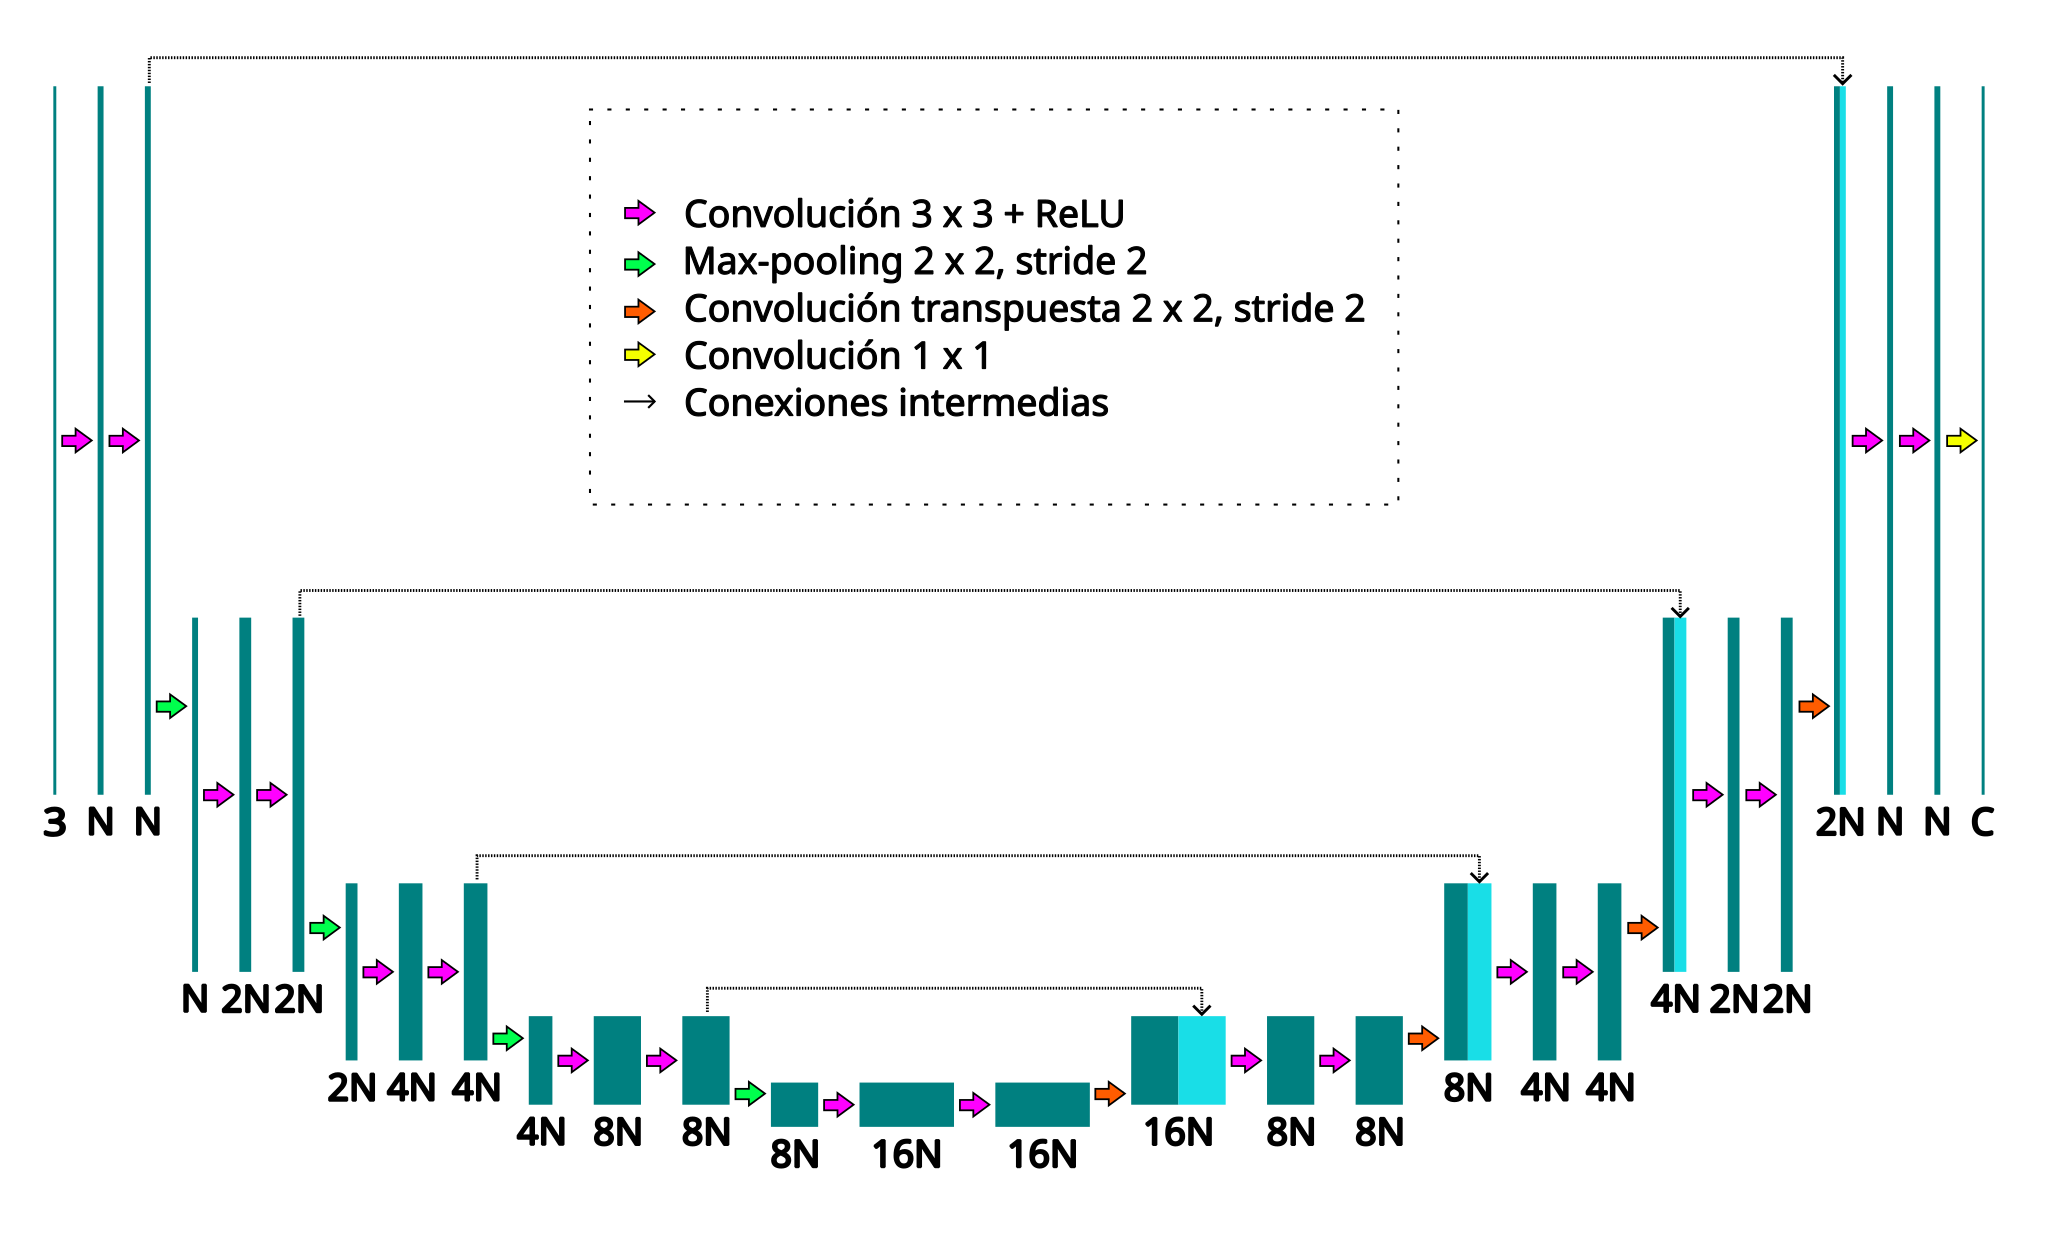
\includegraphics[width=\textwidth]{my_images/metodologia/U-Net.png}\\[1ex]
		\end{minipage}\hfill
		
	\end{columns}
\end{frame}


\begin{frame}{Trabajo Desarrollado: Arquitecturas}
	\begin{columns}[T]
		% Primera columna
		\column{0.5\textwidth}
		\begin{block}{Multi Decoder U-Net}
			\begin{itemize}
					\item Mismo número de etapas decodificadoras como tareas.
			\end{itemize}
		\end{block}
		\begin{center}
			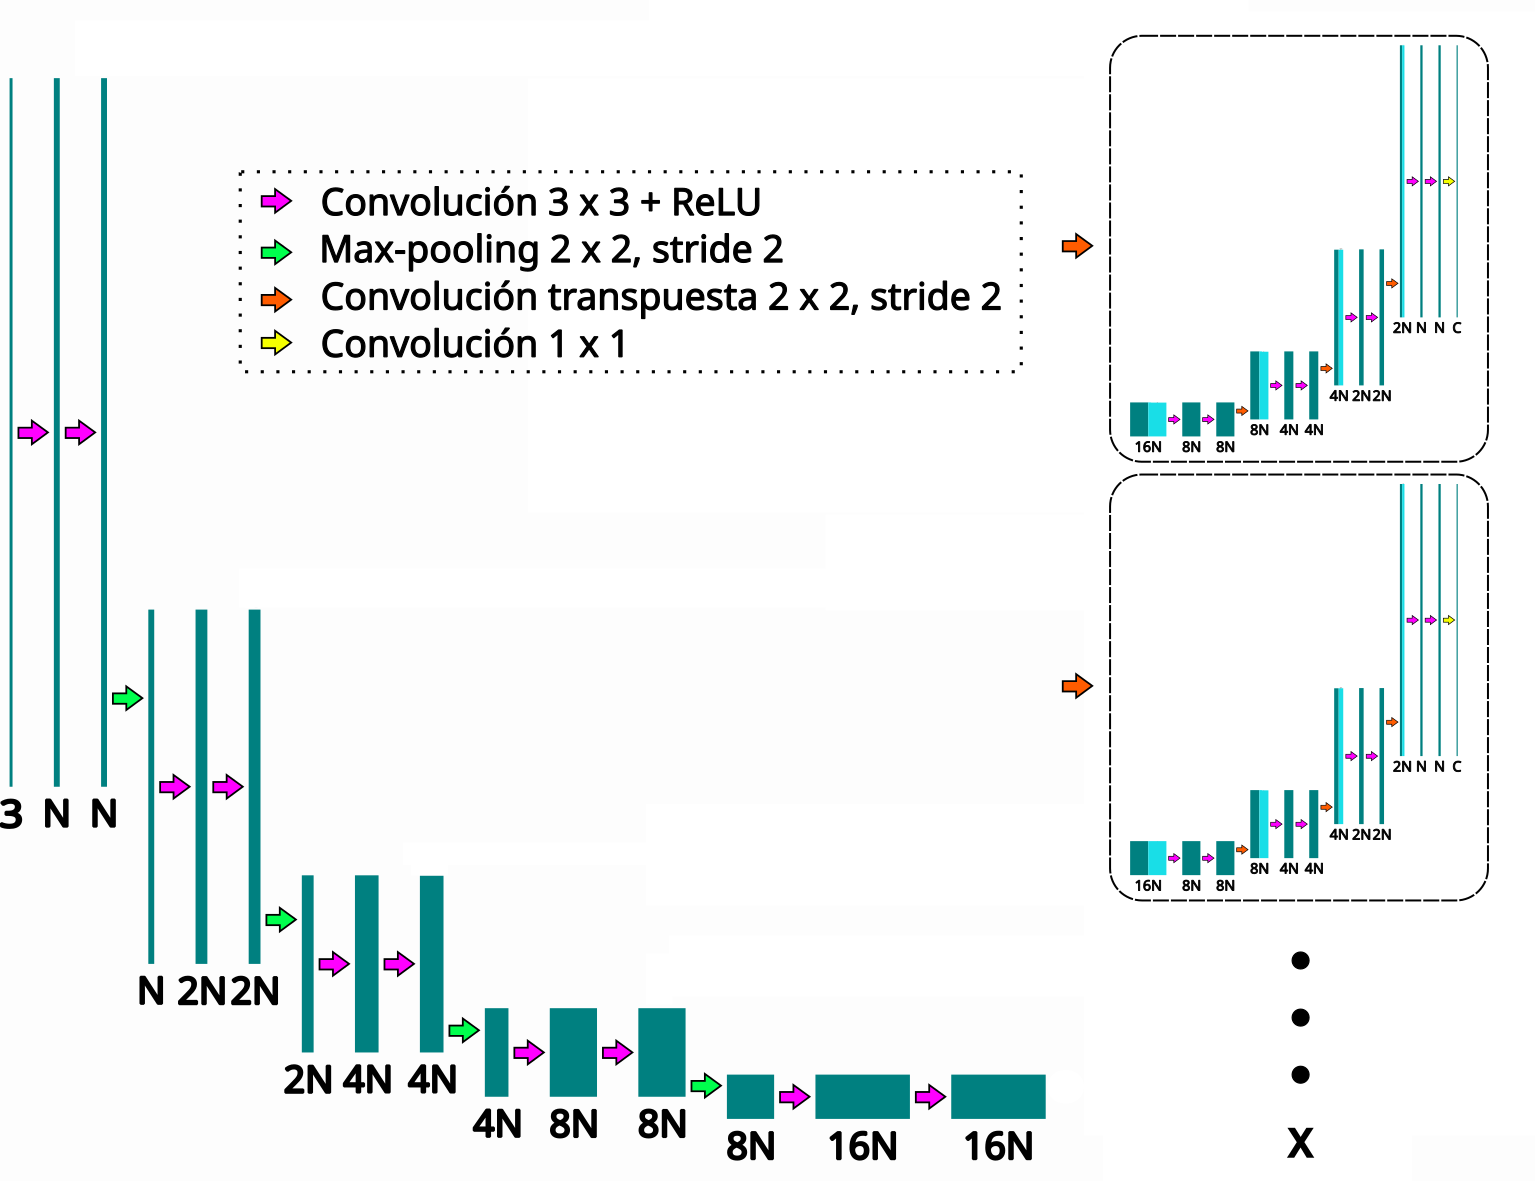
\includegraphics[width=0.8\textwidth]{my_images/metodologia/Multi.png}
		\end{center}
		
		% Segunda columna
		\column{0.5\textwidth}
		\begin{block}{Multi Task U-Net}
			\begin{itemize}

		\item Convoluciones finales con grupos con el mismo número que tareas.

\end{itemize}
		\end{block}
		\begin{center}
			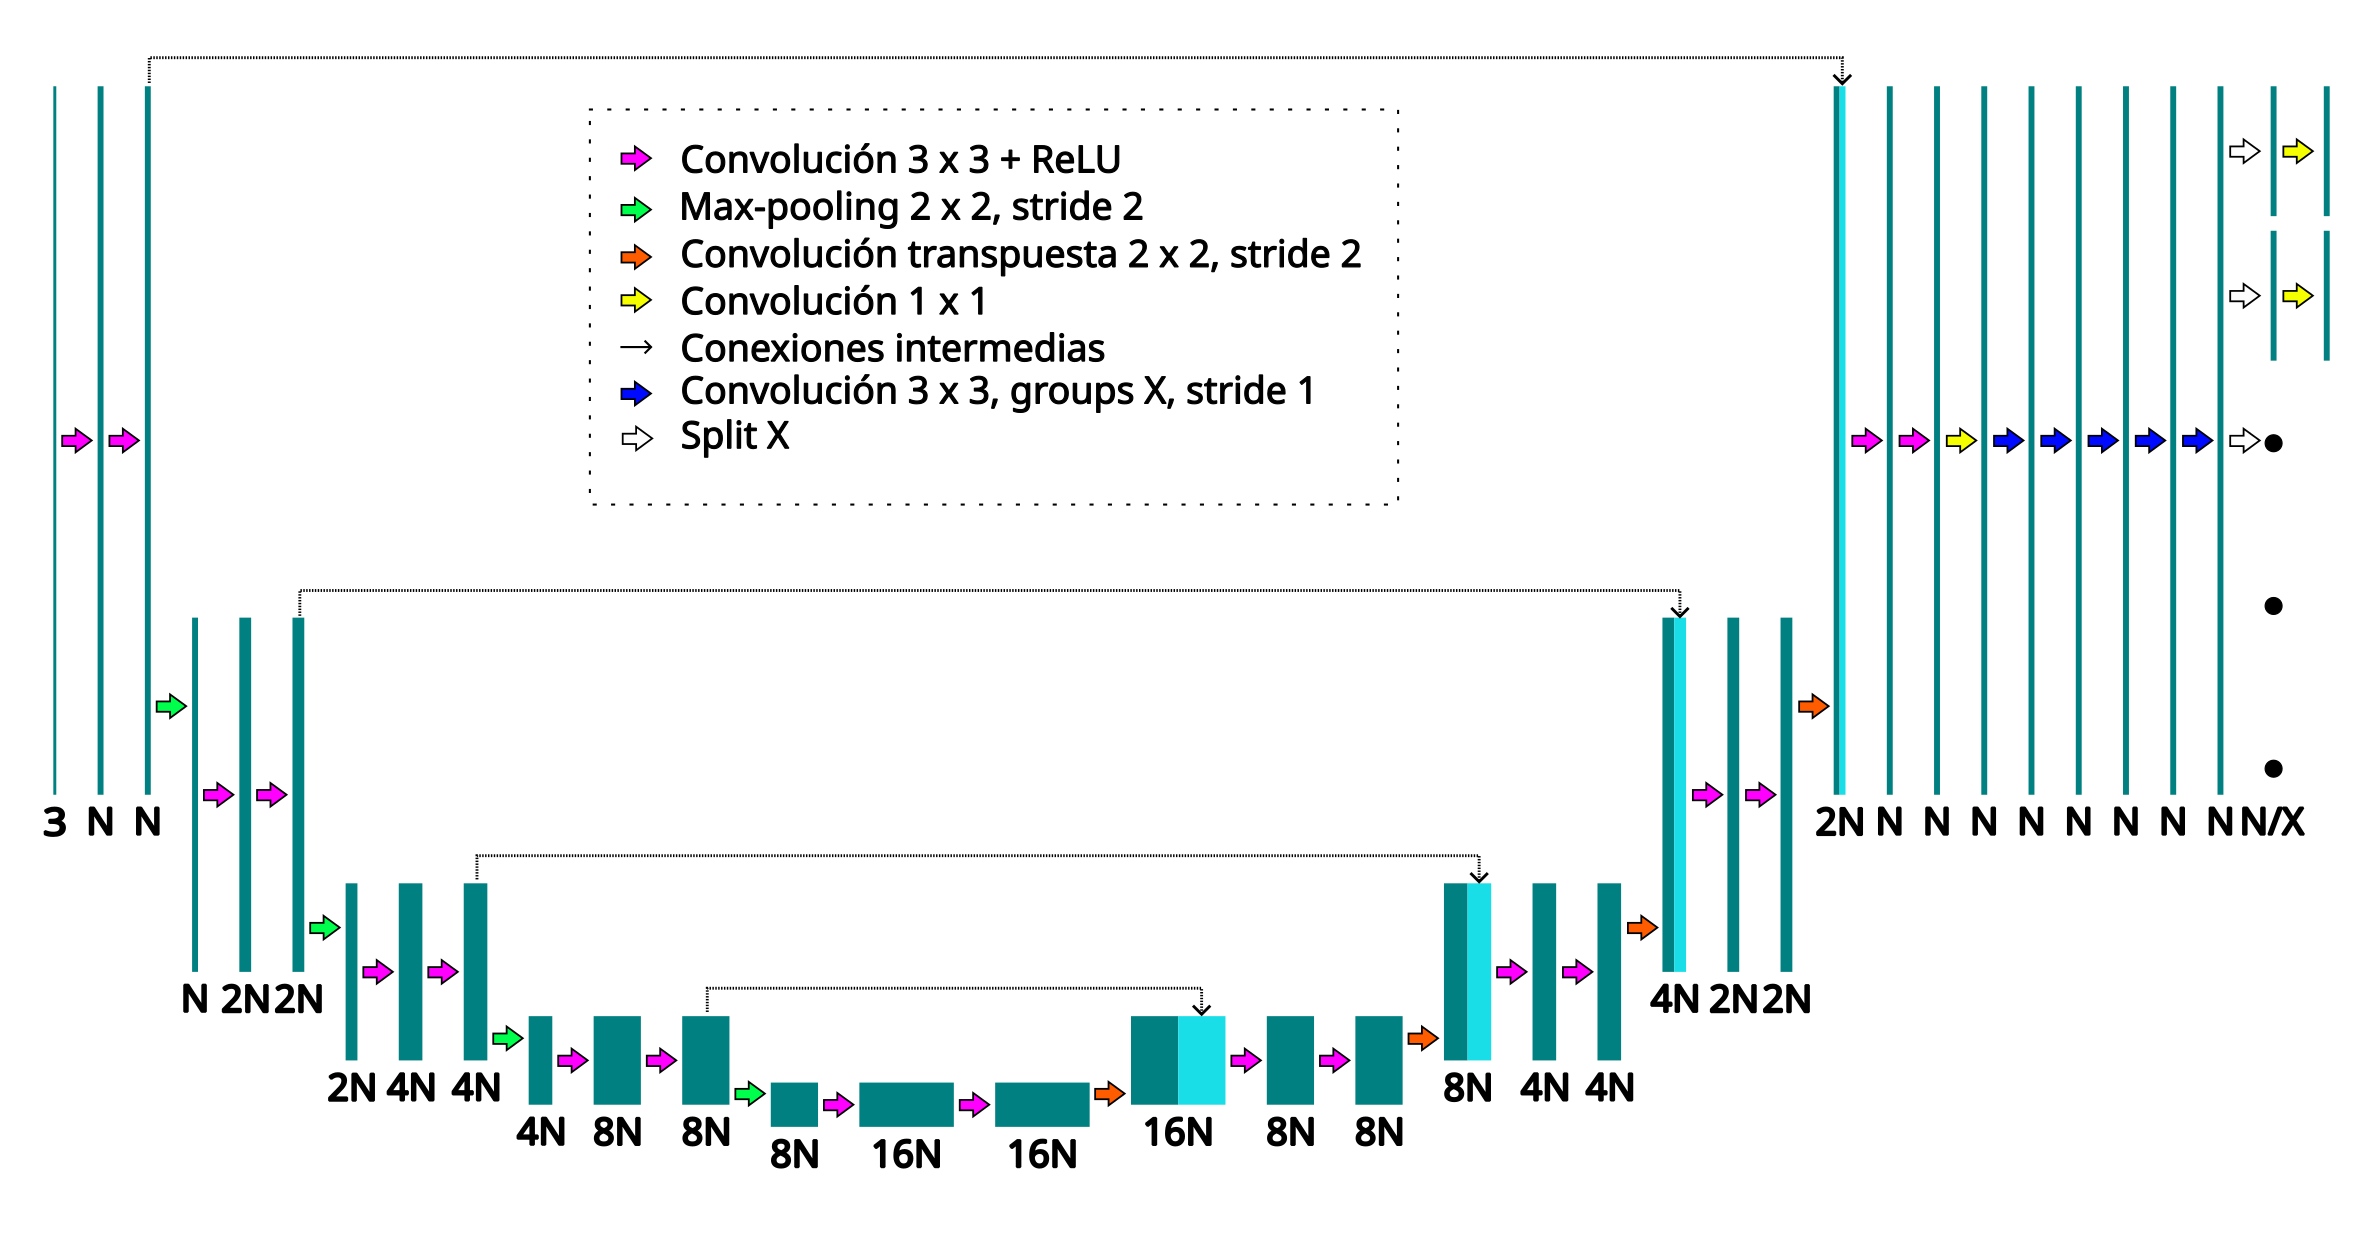
\includegraphics[width=0.8\textwidth]{my_images/metodologia/groups.png}
		\end{center}
	\end{columns}
\end{frame}

%------------------ Conclusións ------------------------%
\section{Experimentación y Resultados}

\begin{comment}
\begin{frame}{Experimentos}
	\begin{columns}[T]
		% Columna izquierda: bloque con la información
		\column{0.45\textwidth}
		\begin{block}{Primera Iteración}
			\begin{enumerate}
				\item Entrenar modelos STL, MTL y MAO con U-NET
				\item Evaluar y comparar resultados
				\begin{itemize}
					\item Se comprueba que los resultados STL son superiores.
				\end{itemize}
			\end{enumerate}
		\end{block}
		
		% Columna derecha: cuadrícula de imágenes con encabezados y etiquetas laterales
		\column{0.55\textwidth}
		\begin{center}
			\setlength{\tabcolsep}{2pt}
			\begin{tabular}{r c c c c c} 
				% Fila de encabezados para cada columna (la primera celda se deja en blanco para la columna de etiquetas)
				&  OD &  FV &  AV &  XB &  AC \\[2mm]
				% Fila 1: etiqueta a la izquierda y 5 imágenes
				STL &
				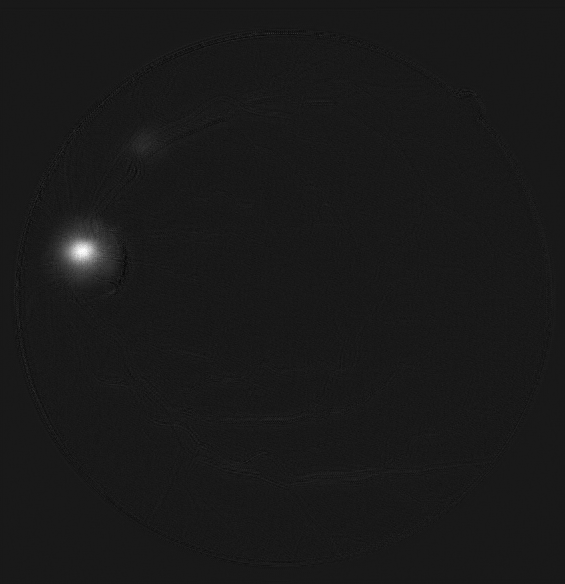
\includegraphics[width=0.15\textwidth]{my_images/video/ODSTL.jpg} &
				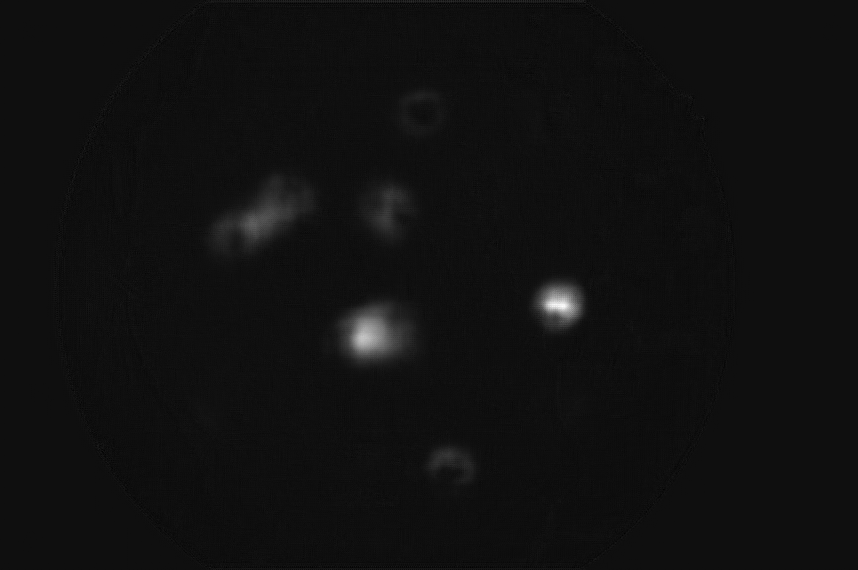
\includegraphics[width=0.15\textwidth]{my_images/video/FOVEASTL.jpg} &
				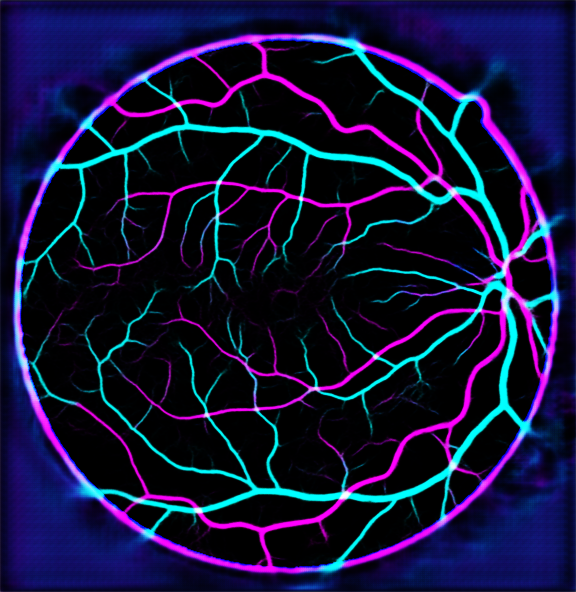
\includegraphics[width=0.15\textwidth]{my_images/video/AVSTL.png} &
				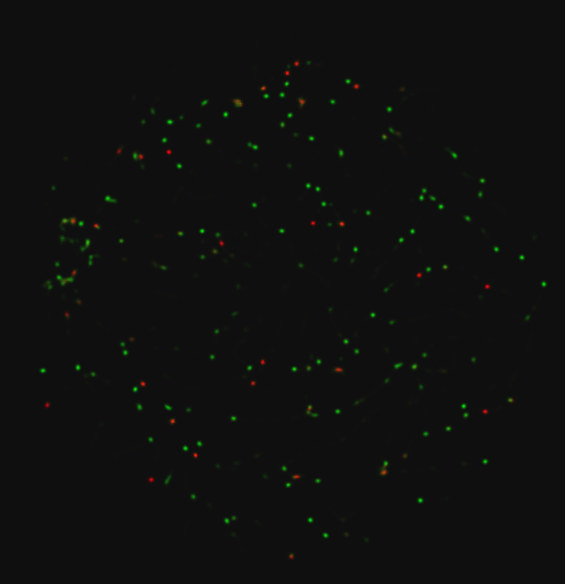
\includegraphics[width=0.15\textwidth]{my_images/video/XBSTL.jpg} &
				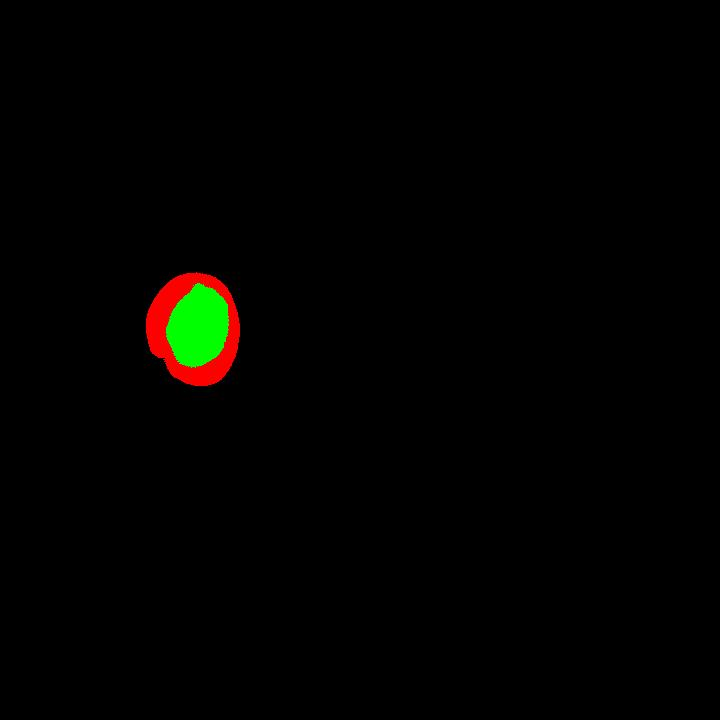
\includegraphics[width=0.15\textwidth]{my_images/video/HARDSTL.jpg} \\[2mm]
				% Fila 2
				MTL &
				\includegraphics[width=0.15\textwidth]{my_images/video/ODUNETMTL.jpg} &
				\includegraphics[width=0.15\textwidth]{my_images/video/FOVEAUNETMTL.jpg} &
				\includegraphics[width=0.15\textwidth]{my_images/video/AVUNETMTL.png} &
				\includegraphics[width=0.15\textwidth]{my_images/video/XBUNETMTL.jpg} &
				\includegraphics[width=0.15\textwidth]{my_images/video/HARDUNETMTL.jpg} \\[2mm]
				% Fila 3
				MAO &
				\includegraphics[width=0.15\textwidth]{my_images/video/ODUNETMAO.jpg} &
				\includegraphics[width=0.15\textwidth]{my_images/video/FOVEAUNETMAO.jpg} &
				\includegraphics[width=0.15\textwidth]{my_images/video/AVUNETMAO.png} &
				\includegraphics[width=0.15\textwidth]{my_images/video/XBUNETMAO.jpg} &
				\includegraphics[width=0.15\textwidth]{my_images/video/SOFTUNETMAO.jpg} \\[2mm]
			\end{tabular}
		\end{center}
	\end{columns}
\end{frame}


\begin{frame}{Experimentos}
	\begin{columns}[T]
		% Columna izquierda: bloque con la información
		\column{0.45\textwidth}
		\begin{block}{Segunda Iteración}
			\begin{enumerate}
				\item Entrenar modelos MTL y MAO con Multi-Decoder U-Net
				\item Evaluar y comparar resultados
				\begin{itemize}
					\item Se comprueba que los resultados mejoran, pero siguen siendo algo inferiores a STL.
				\end{itemize}
			\end{enumerate}
		\end{block}
		
		% Columna derecha: cuadrícula de imágenes con encabezados y etiquetas laterales
		\column{0.55\textwidth}
		\begin{center}
			\setlength{\tabcolsep}{2pt}
			\begin{tabular}{r c c c c c} 
				% Fila de encabezados para cada columna (la primera celda se deja en blanco para la columna de etiquetas)
				&  OD &  FV &  AV &  XB &  AC \\[2mm]
				% Fila 1: etiqueta a la izquierda y 5 imágenes
				STL &
				\includegraphics[width=0.15\textwidth]{my_images/video/ODSTL.jpg} &
				\includegraphics[width=0.15\textwidth]{my_images/video/FOVEASTL.jpg} &
				\includegraphics[width=0.15\textwidth]{my_images/video/AVSTL.png} &
				\includegraphics[width=0.15\textwidth]{my_images/video/XBSTL.jpg} &
				\includegraphics[width=0.15\textwidth]{my_images/video/HARDSTL.jpg} \\[2mm]
				% Fila 2
				MTL &
				\includegraphics[width=0.15\textwidth]{my_images/video/ODMULTIMTL.jpg} &
				\includegraphics[width=0.15\textwidth]{my_images/video/FOVEAMULTIMTL.jpg} &
				\includegraphics[width=0.15\textwidth]{my_images/video/AVMULTIMTL.png} &
				\includegraphics[width=0.15\textwidth]{my_images/video/XBMULTIMTL.jpg} &
				\includegraphics[width=0.15\textwidth]{my_images/video/HARDMULTIMTL.jpg} \\[2mm]
				% Fila 3
				MAO &
				\includegraphics[width=0.15\textwidth]{my_images/video/ODMULTIMAO.jpg} &
				\includegraphics[width=0.15\textwidth]{my_images/video/FOVEAMULTIMAO.jpg} &
				\includegraphics[width=0.15\textwidth]{my_images/video/AVMULTIMAO.png} &
				\includegraphics[width=0.15\textwidth]{my_images/video/XBMULTIMAO.jpg} &
				\includegraphics[width=0.15\textwidth]{my_images/video/HARDMULTIMAO.jpg} \\[2mm]
			\end{tabular}
		\end{center}
	\end{columns}
\end{frame}

\begin{frame}{Experimentos}
	\raisebox{1cm}{
		\begin{columns}[T]
			% Columna izquierda: bloque con la información
			\column{0.45\textwidth}
			\begin{block}{Tercera Iteración}
				\begin{enumerate}
					\item Entrenar modelos MTL y MAO con Multi-Task U-Net
					\item Evaluar y comparar resultados
					\begin{itemize}
						\item Se comprueba que los resultados son similares a la anterior iteración.
					\end{itemize}
				\end{enumerate}
			\end{block}
			
			% Columna derecha: cuadrícula de imágenes con encabezados y etiquetas laterales
			\column{0.55\textwidth}
			\begin{center}
				\setlength{\tabcolsep}{2pt}
				\begin{tabular}{r c c c c c} 
					% Fila de encabezados para cada columna (la primera celda se deja en blanco para la columna de etiquetas)
					&  OD &  FV &  AV &  XB &  AC \\[2mm]
					% Fila 1: etiqueta a la izquierda y 5 imágenes
					STL &
					\includegraphics[width=0.15\textwidth]{my_images/video/ODSTL.jpg} &
					\includegraphics[width=0.15\textwidth]{my_images/video/FOVEASTL.jpg} &
					\includegraphics[width=0.15\textwidth]{my_images/video/AVSTL.png} &
					\includegraphics[width=0.15\textwidth]{my_images/video/XBSTL.jpg} &
					\includegraphics[width=0.15\textwidth]{my_images/video/HARDSTL.jpg} \\[2mm]
					% Fila 2
					MTL &
					\includegraphics[width=0.15\textwidth]{my_images/video/ODTASKMTL.jpg} &
					\includegraphics[width=0.15\textwidth]{my_images/video/FOVEATASKMTL.jpg} &
					\includegraphics[width=0.15\textwidth]{my_images/video/AVTASKMTL.png} &
					\includegraphics[width=0.15\textwidth]{my_images/video/XBTASKMTL.jpg} &
					\includegraphics[width=0.15\textwidth]{my_images/video/HARDTASKMTL.jpg} \\[2mm]
					% Fila 3
					MAO &
					\includegraphics[width=0.15\textwidth]{my_images/video/ODTASKMAO.jpg} &
					\includegraphics[width=0.15\textwidth]{my_images/video/FOVEATASKMAO.jpg} &
					\includegraphics[width=0.15\textwidth]{my_images/video/AVTASKMAO.png} &
					\includegraphics[width=0.15\textwidth]{my_images/video/XBTASKMAO.jpg} &
					\includegraphics[width=0.15\textwidth]{my_images/video/HARDTASKMAO.jpg} \\[2mm]
				\end{tabular}
			\end{center}
	\end{columns}}
\end{frame}
\end{comment}
\begin{frame}{Experimentación y Resultados: Iteraciones}
	\scalebox{0.8}{
		\begin{minipage}{1.25\textwidth} % Ajusta el ancho según necesites
			\begin{block}<1->{Primera Iteración}
				\begin{enumerate}
					\item Entrenar modelos STL, MTL y MAO con U-NET
					\item Evaluar y comparar resultados
					\begin{itemize}
						\item Se comprueba que los resultados STL son superiores.
					\end{itemize}
				\end{enumerate}
			\end{block}
			\begin{block}<2->{Segunda Iteración}
				\begin{enumerate}
					\item Entrenar modelos MTL y MAO con Multi-Decoder U-Net
					\item Evaluar y comparar resultados
					\begin{itemize}
						\item Se comprueba que los resultados mejoran, pero siguen siendo algo inferiores a STL.
					\end{itemize}
				\end{enumerate}
			\end{block}
			\begin{block}<3->{Tercera Iteración}
				\begin{enumerate}
					\item Entrenar modelos MTL y MAO con Multi-Task U-Net
					\item Evaluar y comparar resultados
					\begin{itemize}
						\item Se comprueba que los resultados son similares a la anterior iteración.
					\end{itemize}
				\end{enumerate}
			\end{block}
		\end{minipage}
	}
\end{frame}

\begin{frame}{Experimentación y Resultados: Conjunto de datos}
	\vspace{0.6cm} % Espacio vertical antes del bloque grande
	
	\scalebox{0.9}{%
		\begin{minipage}{\textwidth}
			% Primera fila de bloques
			\begin{columns}[T,onlytextwidth]
				\column{0.45\textwidth}
				\begin{block}{DRIVE/RITE}
					\begin{itemize}
						\item 40 imágenes.
						\item 565 × 584 píxeles
						\item Tareas:
							\begin{itemize}
								\item Detección del Disco Óptico.
								\item Detección de Cruces y bifurcaciones.
								\item Segmentación de Arterias y Venas.
							\end{itemize}
					\end{itemize}
				\end{block}
				\column{0.48\textwidth}
				\begin{block}{IDRiD}
					\begin{itemize}
						\item 516 imágenes.
						\item 858 × 570 píxeles
						\item Tareas:
						\begin{itemize}
							\item Detección Fóvea.
						\end{itemize}
					\end{itemize}
				\end{block}
			\end{columns}
			
			\vspace{0.1cm} % Espacio vertical entre filas
			
			% Segunda fila de bloques
			\begin{columns}[T,onlytextwidth]
				\column{0.45\textwidth}

				\column{0.48\textwidth}
				\vspace{-2cm}
				\begin{block}{REFUGE}
	\begin{itemize}
		\item 1200 imágenes.
		\item 720 × 697 píxeles
		\item Tareas:
		\begin{itemize}
			\item Segmentación de Copa y Anillo del Disco Óptico.
		\end{itemize}
		
	\end{itemize}
\end{block}
			\end{columns}
		\end{minipage}
	}
\end{frame}

\begin{frame}{Experimentación y Resultados: Conjunto de datos}
	\begin{block}{Conjunto de datos en MTL}
¿Cómo entrenar un modelo MTL si no hay un dataset con todo unificado?
		\begin{itemize}
			\item 11 canales de salida
			\begin{itemize}
				\item 1 canal Disco óptico
				\item 1 canal Fóvea
				\item 3 canales Arterias y Venas
				\item 3 canales Cruces y bifurcaciones
				\item 3 canales Anillo y Copa del Disco óptico
			\end{itemize}				
		\item Cada iteración en entrenamiento, se concatena una imagen de cada dataset.
		\begin{itemize}
			\item Para poder hacer esto reescalamos las imágenes.
		\end{itemize}
		\item Calculamos la pérdida de los canales que tenemos etiqueta.
		\end{itemize}
	\end{block}
\end{frame}

\begin{comment}
	
\begin{frame}{Experimentos}
		\vspace{0.6cm}
		\centering
	\scalebox{0.8}{%
		\begin{minipage}{\textwidth}
			% Primera fila de bloques
			\begin{columns}[T,onlytextwidth]
				\column{0.45\textwidth}
				\begin{block}{DRIVE}
						\begin{itemize}
							\item Disco óptico.
							\item Cruces y bifurcaciones.
						\end{itemize}
				\end{block}
				\column{0.48\textwidth}
				\begin{block}{IDRiD}
					\begin{itemize}
							\item Fóvea.
						\end{itemize}
					
				\end{block}
			\end{columns}
			
			\vspace{0.1cm} % Espacio vertical entre filas
			
			% Segunda fila de bloques
			\begin{columns}[T,onlytextwidth]
				\column{0.45\textwidth}
				\begin{block}{REFUGE}
						\begin{itemize}
							\item Anillo y copa del disco óptico.
						\end{itemize}
				\end{block}
				\column{0.48\textwidth}
				\begin{block}{RITE}
						\begin{itemize}
							\item Segmentación de arterias o venas.
						\end{itemize}
				\end{block}
			\end{columns}
			
			\vspace{0.2cm} % Espacio vertical antes del bloque grande
			
			% Bloque grande que ocupa todo el ancho
	\begin{block}{Conjunto Unificado}
	\begin{itemize}
		\item Se hacen modificaciones:
		\begin{itemize}
			
			\item DRIVE y RITE unidos en un solo dataset.
			\item Datasets modificados para mejorar rendimiento.
			
			\item Disminuir la cantidad de lotes de datos, deriva en una menor demanda de memoria GPU.
		\end{itemize}
			\item MTL
			\item MAO
	\end{itemize}
\end{block}
			
		\end{minipage}
	}
\end{frame}

\begin{frame}
	% Primera fila de bloques
	\begin{block}{Modificaciones}
		\begin{itemize}
			
			\item DRIVE y RITE unidos en un solo dataset.
			\item Datasets modificados para mejorar rendimiento.
			\begin{itemize}
				\item Disminuir la cantidad de lotes de datos, deriva en una menor demanda de memoria GPU.
			\end{itemize}
		\end{itemize}
	\end{block}
\end{frame}
\end{comment}

\begin{frame}{Experimentación y Resultados: Detalles experimentales}
	\scalebox{0.88}{%
		\begin{minipage}{1.25\linewidth}
			\begin{block}{}
				\begin{itemize}
					\item Los entrenamientos se configuran para mejorar la comparación.
					
					\item Aumento de datos:
					\begin{itemize}
						\item Random Horizontal Flip
						\item Random Vertical Flip
						\item Random HSV
						\item Random Affine
					\end{itemize}
	
						\item Tasa de aprendizaje constante de $1 \times 10^{-4}$
						\item 500 épocas.
						\item 100 imágenes por época.
					\item Optimizador ADAM:
					\begin{itemize}
						\item En MAO está implícito.
					\end{itemize}
				\end{itemize}
			\end{block}
		\end{minipage}
	}
	
\end{frame}




\begin{frame}{Experimentación y Resultados: Evaluación}
	\begin{columns}[t] % 't' alinea las columnas en la parte superior
		
		% Primera columna
		\column{0.5\textwidth}
		\scalebox{0.8}{%
			\begin{minipage}{\linewidth}
				\begin{block}{Disco Óptico}
					\begin{enumerate}
						\item Error promedio de la localización del Disco.
						\item Desviación estándar.
						\item Precisión en relación a un umbral.
					\end{enumerate}
				\end{block}

				\begin{block}{Arterias y Venas}
					\begin{enumerate}
						\item Curva ROC.
						\item Curva PR.
					\end{enumerate}
				\end{block}

				\begin{block}{Cruces y Bifurcaciones}
					\begin{enumerate}
						\item F1-Score.
						\item Precisión media.
					\end{enumerate}
				\end{block}
			\end{minipage}%
		}
		
		% Segunda columna
		\column{0.5\textwidth}
		\scalebox{0.8}{%
			\begin{minipage}{\linewidth}
				\begin{block}{Fóvea}
					\begin{enumerate}
						\item Error promedio de la localización de la Fóvea.
						\item Desviación estándar.
						\item Precisión en relación a un umbral.
					\end{enumerate}
				\end{block}
			
				\begin{block}{Anillo y Copa}
					\begin{enumerate}
						\item Mean dice.
						\item Mean Jaccard.
						\item Curva PR.
					\end{enumerate}
				\end{block}
	
				
				\begin{block}{Evaluación Cualitativa}
					\begin{enumerate}
						\item Comparación imagen a imagen de las diferentes tareas.
					\end{enumerate}
				\end{block}
			\end{minipage}%
		}
		
	\end{columns}
\end{frame}


\begin{frame}
	\centering
	\textbf{\huge Resultados.}
\end{frame}

\begin{frame}{Experimentación y Resultados: Cruces y Bifurcaciones}
	\begin{itemize}
		\only<1-2>{\item Resultados MTL normalmente inferiores a STL.}
		\only<2->{\item Multi-Decoder U-Net sin MAO supera a STL en el conjunto de cruces y bifurcaciones}
	\end{itemize}
	
	\only<1>{
		\begin{block}{Cruces}
			\begin{table}[h]
				\centering
				\small
				\begin{tabular}{lcc}
					\hline
					Modelo   & f1-score & Average Precision \\ \hline
					MultiMTL & 68.12    & 67.54             \\
					STL      & 72.12    & 72.47             \\ \hline
				\end{tabular}
			\end{table}
		\end{block}
		
				\begin{block}{Bifurcaciones}
			\begin{table}[h]
				\centering
				\small
				\begin{tabular}{lcc}
					\hline
					Modelo   & f1-score & Average Precision \\ \hline
					MultiMTL & 65.96    & 68.09             \\
					STL      & 67.94    & 68.29             \\ \hline
				\end{tabular}
			\end{table}
		\end{block}
	}
	

	\only<2>{
		\begin{block}{Cruces y Bifurcaciones}
			\begin{table}[h]
				\centering
				\small
				\begin{tabular}{lcc}
					\hline
					Modelo   & f1-score & Average Precision \\ \hline
					MultiMTL & 76.78    & 77.35             \\
					STL      & 74.10    & 75.36             \\ \hline
				\end{tabular}
			\end{table}
		\end{block}
	}
\end{frame}

\begin{frame}{Experimentación y Resultados: Cruces y Bifurcaciones}
	\centering
	\begin{minipage}[b]{0.13\textwidth}
		\centering
		STL\\[0.2cm]
		\includegraphics[width=\linewidth]{my_images/video/XBSTL.jpg}
	\end{minipage}\hfill
	\begin{minipage}[b]{0.13\textwidth}
		\centering
		U-Net MTL\\[0.2cm]
		\includegraphics[width=\linewidth]{my_images/video/XBUNETMTL.jpg}
	\end{minipage}\hfill
	\begin{minipage}[b]{0.13\textwidth}
		\centering
		U-Net MAO\\[0.2cm]
		\includegraphics[width=\linewidth]{my_images/video/XBUNETMAO.jpg}
	\end{minipage}\hfill
	\begin{minipage}[b]{0.13\textwidth}
		\centering
		Multi-Task MTL\\[0.2cm]
		\includegraphics[width=\linewidth]{my_images/video/XBTASKMTL.jpg}
	\end{minipage}\hfill
	\begin{minipage}[b]{0.13\textwidth}
		\centering
		Multi-Task MAO\\[0.2cm]
		\includegraphics[width=\linewidth]{my_images/video/XBTASKMAO.jpg}
	\end{minipage}\hfill
	\begin{minipage}[b]{0.13\textwidth}
		\centering
		Multi-Decoder MTL\\[0.2cm]
		\includegraphics[width=\linewidth]{my_images/video/XBMULTIMTL.jpg}
	\end{minipage}\hfill
	\begin{minipage}[b]{0.13\textwidth}
		\centering
		Multi-Decoder MAO\\[0.2cm]
		\includegraphics[width=\linewidth]{my_images/video/XBMULTIMAO.jpg}
	\end{minipage}
\end{frame}

\begin{frame}{Experimentación y Resultados: Disco Óptico}
	\begin{itemize}
		\only<1-2>{\item Resultados MTL superiores a STL.}
		\only<2->{\item Aún así, no todos tienen resultados tan buenos.}
	\end{itemize}
	
	\only<1>{
		\begin{block}{}
			\begin{table}[h!]
				\centering
				\resizebox{\textwidth}{!}{%
					\begin{tabular}{@{}lccccc@{}}
						\toprule
						\textbf{Modelo} & \textbf{Precisión ($R$)} & \textbf{Precisión ($R/2$)} & \textbf{Precisión ($R/4$)} & \textbf{Error promedio (px)} & \textbf{Desviación estándar (px)} \\
						\midrule
						TaskMAO & 100\% & 100\% & 100\% & 3.77 & 2.16 \\
						\bottomrule
					\end{tabular}%
				}
				
				\label{tab:results}
			\end{table}
		\end{block}
	}
	
	\only<2>{
		\begin{table}[h!]
			\centering
			\resizebox{\textwidth}{!}{%
				\begin{tabular}{@{}lccccc@{}}
					\toprule
					\textbf{Modelo} & \textbf{Precisión ($R$)} & \textbf{Precisión ($R/2$)} & \textbf{Precisión ($R/4$)} & \textbf{Error promedio (px)} & \textbf{Desviación estándar (px)} \\
					\midrule
					MultiMTL & 100\% & 100\% & 95\% & 5.52 & 3.41 \\
					UNetMTL & 100\% & 100\% & 90\% & 5.14 & 2.77 \\
					STL      & 100\% & 90\% & 85\% & 7.81 & 5.90 \\
					\bottomrule
				\end{tabular}%
			}
			
			\label{tab:results}
		\end{table}
	}
	
\end{frame}

\begin{frame}{Experimentación y Resultados: Disco Óptico}
	\centering
	\begin{minipage}[b]{0.13\textwidth}
		\centering
		STL\\[0.2cm]
		\includegraphics[width=\linewidth]{my_images/video/ODSTL.jpg}
	\end{minipage}\hfill
	\begin{minipage}[b]{0.13\textwidth}
		\centering
		U-Net MTL\\[0.2cm]
		\includegraphics[width=\linewidth]{my_images/video/ODUNETMTL.jpg}
	\end{minipage}\hfill
	\begin{minipage}[b]{0.13\textwidth}
		\centering
		U-Net MAO\\[0.2cm]
		\includegraphics[width=\linewidth]{my_images/video/ODUNETMAO.jpg}
	\end{minipage}\hfill
	\begin{minipage}[b]{0.13\textwidth}
		\centering
		Multi-Task MTL\\[0.2cm]
		\includegraphics[width=\linewidth]{my_images/video/ODTASKMTL.jpg}
	\end{minipage}\hfill
	\begin{minipage}[b]{0.13\textwidth}
		\centering
		Multi-Task MAO\\[0.2cm]
		\includegraphics[width=\linewidth]{my_images/video/ODTASKMAO.jpg}
	\end{minipage}\hfill
	\begin{minipage}[b]{0.13\textwidth}
		\centering
		Multi-Decoder MTL\\[0.2cm]
		\includegraphics[width=\linewidth]{my_images/video/ODMULTIMTL.jpg}
	\end{minipage}\hfill
	\begin{minipage}[b]{0.13\textwidth}
		\centering
		Multi-Decoder MAO\\[0.2cm]
		\includegraphics[width=\linewidth]{my_images/video/ODMULTIMAO.jpg}
	\end{minipage}
\end{frame}


\begin{frame}{Experimentación y Resultados: Fóvea}

	\begin{itemize}
	\only<1>{\item Resultados con MAO superiores al resto de resultados.}
\end{itemize}

\only<1>{
	\begin{block}{}
		
		\begin{table}[h!]
			\centering
			\resizebox{\textwidth}{!}{%
				\begin{tabular}{@{}lccccc@{}}
					\toprule
					\textbf{Modelo} & \textbf{Precisión ($R$)} & \textbf{Precisión ($R/2$)} & \textbf{Precisión ($R/4$)} & \textbf{Error promedio (px)} & \textbf{Desviación estándar (px)} \\
					\midrule
					MultiMAO & 93.14\% & 88.24\% & 78.43\% & 16.96 & 37.86 \\
					TaskMAO & 91.18\% & 84.31\% & 73.53\% & 19.24 & 42.47 \\
					\bottomrule
				\end{tabular}%
			}
			
			\label{tab:fovea_results}
		\end{table}
	\end{block}
}
	
\end{frame}

\begin{frame}{Experimentación y Resultados: Fóvea}
	\centering
	\begin{minipage}[b]{0.13\textwidth}
		\centering
		STL\\[0.2cm]
		\includegraphics[width=\linewidth]{my_images/video/FOVEASTL.jpg}
	\end{minipage}\hfill
	\begin{minipage}[b]{0.13\textwidth}
		\centering
		U-Net MTL\\[0.2cm]
		\includegraphics[width=\linewidth]{my_images/video/FOVEAUNETMTL.jpg}
	\end{minipage}\hfill
	\begin{minipage}[b]{0.13\textwidth}
		\centering
		U-Net MAO\\[0.2cm]
		\includegraphics[width=\linewidth]{my_images/video/FOVEAUNETMAO.jpg}
	\end{minipage}\hfill
	\begin{minipage}[b]{0.13\textwidth}
		\centering
		Multi-Task MTL\\[0.2cm]
		\includegraphics[width=\linewidth]{my_images/video/FOVEATASKMTL.jpg}
	\end{minipage}\hfill
	\begin{minipage}[b]{0.13\textwidth}
		\centering
		Multi-Task MAO\\[0.2cm]
		\includegraphics[width=\linewidth]{my_images/video/FOVEATASKMAO.jpg}
	\end{minipage}\hfill
	\begin{minipage}[b]{0.13\textwidth}
		\centering
		Multi-Decoder MTL\\[0.2cm]
		\includegraphics[width=\linewidth]{my_images/video/FOVEAMULTIMTL.jpg}
	\end{minipage}\hfill
	\begin{minipage}[b]{0.13\textwidth}
		\centering
		Multi-Decoder MAO\\[0.2cm]
		\includegraphics[width=\linewidth]{my_images/video/FOVEAMULTIMAO.jpg}
	\end{minipage}
\end{frame}




\begin{frame}{Experimentación y Resultados: Arterias y Venas}
	
	\begin{itemize}
		\only<1>{\item Resultados inferiores de MTL frente STL en Venas.}
		\only<2>{\item Aunque superiores o similares en Arterias y Vasos.}
		\only<3>{\item Único resultado donde U-Net con MAO tiene un resultado aceptable.}
	\end{itemize}
	
	\only<1>{
		\begin{block}{}
		\begin{table}[h!]
			\centering
			\resizebox{0.4\textwidth}{!}{%
				\begin{tabular}{@{}lcc@{}}
					\toprule
					\textbf{Model} & \multicolumn{2}{c}{\textbf{Venas}}\\
					\cmidrule(lr){2-3} 
					& AUC-ROC (\%) & AUC-PR (\%) \\
					\midrule
					UNetMTL & 95.93 & 76.24 \\
					TI      & 97.45 & 84.84 \\
					\bottomrule
				\end{tabular}%
			}
		\end{table}
		
		\end{block}
	}
	
\only<2>{
	\begin{block}{}
		\begin{table}[h!]
			\centering
			\label{tab:subresultadosAV}
						\resizebox{0.6\textwidth}{!}{%
			\begin{tabular}{lcccc}
				\toprule
				\textbf{Model} & \multicolumn{2}{c}{\textbf{Arterias}} & \multicolumn{2}{c}{\textbf{Vasos}} \\
				\cmidrule(lr){2-3} \cmidrule(lr){4-5}
				& AUC-ROC (\%) & AUC-PR (\%) & AUC-ROC (\%) & AUC-PR (\%) \\
				\midrule
				UNetMTL      & 97.01 & 82.67 & 97.82 & 91.33 \\
				TI           & 96.93 & 80.10 & 97.90 & 91.59 \\
				\bottomrule
			\end{tabular}
		}
		\end{table}
	\end{block}
}

	\only<3>{
		\begin{block}{}
			\begin{table}[h!]
				\centering
				\label{tab:subresultadosAV}
				\resizebox{\textwidth}{!}{%
		\begin{tabular}{lcccccc}
			\toprule
			\textbf{Model} & \multicolumn{2}{c}{\textbf{Venas}} & \multicolumn{2}{c}{\textbf{Arterias}} & \multicolumn{2}{c}{\textbf{Vasos}} \\
			\cmidrule(lr){2-3} \cmidrule(lr){4-5} \cmidrule(lr){6-7}
			& AUC-ROC (\%) & AUC-PR (\%) & AUC-ROC (\%) & AUC-PR (\%) & AUC-ROC (\%) & AUC-PR (\%) \\
			\midrule
			UNetMAO  & 74.01 & 22.54 & 67.94 & 11.87 & 72.22 & 32.56 \\
			\bottomrule
		\end{tabular}%
				}
			\end{table}
		\end{block}
	}
\end{frame}



\begin{frame}{Experimentación y Resultados: Arterias y Venas}
	\centering
	\begin{minipage}[b]{0.13\textwidth}
		\centering
		STL\\[0.2cm]
		\includegraphics[width=\linewidth]{my_images/video/AVSTL.png}
	\end{minipage}\hfill
	\begin{minipage}[b]{0.13\textwidth}
		\centering
		U-Net MTL\\[0.2cm]
		\includegraphics[width=\linewidth]{my_images/video/AVUNETMTL.png}
	\end{minipage}\hfill
	\begin{minipage}[b]{0.13\textwidth}
		\centering
		U-Net MAO\\[0.2cm]
		\includegraphics[width=\linewidth]{my_images/video/AVUNETMAO.png}
	\end{minipage}\hfill
	\begin{minipage}[b]{0.13\textwidth}
		\centering
		Multi-Task MTL\\[0.2cm]
		\includegraphics[width=\linewidth]{my_images/video/AVTASKMTL.png}
	\end{minipage}\hfill
	\begin{minipage}[b]{0.13\textwidth}
		\centering
		Multi-Task MAO\\[0.2cm]
		\includegraphics[width=\linewidth]{my_images/video/AVTASKMAO.png}
	\end{minipage}\hfill
	\begin{minipage}[b]{0.13\textwidth}
		\centering
		Multi-Decoder MTL\\[0.2cm]
		\includegraphics[width=\linewidth]{my_images/video/AVMULTIMTL.png}
	\end{minipage}\hfill
	\begin{minipage}[b]{0.13\textwidth}
		\centering
		Multi-Decoder MAO\\[0.2cm]
		\includegraphics[width=\linewidth]{my_images/video/AVMULTIMAO.png}
	\end{minipage}
\end{frame}



\begin{frame}{Experimentación y Resultados: Copa y Anillo}
	
	\begin{itemize}
		\only<1>{\item Resultados similares o superiores e Anillo pero inferiores en Copa}
	\end{itemize}
	
	\only<1>{
		\begin{block}{}
			
			\begin{table}[h!]
				\centering
				\label{tab:resultadosPR5_}
				\resizebox{\textwidth}{!}{%
					\begin{tabular}{lcccccc}
						\toprule
						\textbf{Estructura} & \multicolumn{3}{c}{\textbf{Anillo}} & \multicolumn{3}{c}{\textbf{COPA}} \\
						\cmidrule(lr){2-4} \cmidrule(lr){5-7} 
						& mean dice (\%) & mean jaccard (\%) & PR-AUC (\%) & mean dice (\%) & mean jaccard (\%) & PR-AUC (\%) \\
						\midrule
						MultiMAO  & 94.95 & 90.46 & 99.18 & 83.22 & 72.21 & 91.98 \\
						STL  & 94.51 & 89.73 & 99.14 & 85.69 & 75.52 & 94.87 \\
						\bottomrule
					\end{tabular}%
				}
			\end{table}
		\end{block}
	}
	
\end{frame}

\begin{frame}{Experimentación y Resultados: Copa y Anillo}
	\centering
	\begin{minipage}[b]{0.13\textwidth}
		\centering
		STL\\[0.2cm]
		\includegraphics[width=\linewidth]{my_images/video/HARDSTL.jpg}
	\end{minipage}\hfill
	\begin{minipage}[b]{0.13\textwidth}
		\centering
		U-Net MTL\\[0.2cm]
		\includegraphics[width=\linewidth]{my_images/video/HARDUNETMTL.jpg}
	\end{minipage}\hfill
	\begin{minipage}[b]{0.13\textwidth}
		\centering
		U-Net MAO\\[0.2cm]
		\includegraphics[width=\linewidth]{my_images/video/SOFTUNETMAO.jpg}
	\end{minipage}\hfill
	\begin{minipage}[b]{0.13\textwidth}
		\centering
		Multi-Task MTL\\[0.2cm]
		\includegraphics[width=\linewidth]{my_images/video/HARDTASKMTL.jpg}
	\end{minipage}\hfill
	\begin{minipage}[b]{0.13\textwidth}
		\centering
		Multi-Task MAO\\[0.2cm]
		\includegraphics[width=\linewidth]{my_images/video/HARDTASKMAO.jpg}
	\end{minipage}\hfill
	\begin{minipage}[b]{0.13\textwidth}
		\centering
		Multi-Decoder MTL\\[0.2cm]
		\includegraphics[width=\linewidth]{my_images/video/HARDMULTIMTL.jpg}
	\end{minipage}\hfill
	\begin{minipage}[b]{0.13\textwidth}
		\centering
		Multi-Decoder MAO\\[0.2cm]
		\includegraphics[width=\linewidth]{my_images/video/HARDMULTIMAO.jpg}
	\end{minipage}
\end{frame}

\begin{frame}{Experimentos y Resultados: Conclusiones}
	\begin{columns}[T]
		
		\column{0.5\textwidth}
		\vspace{-0.4cm}
		\begin{block}{}
			\begin{enumerate}
				\item Bajo las condiciones de entrenamiento propuestas, los modelos STL son superiores.
				\begin{itemize}
					\item Las tareas donde tarda más en empezar el sobreentrenamiento, los resultados compiten con STL.
				\end{itemize}
				\item MAO es dependiente de la arquitectura utilizada.
				\begin{itemize}
					\item El mal rendimiento de la U-Net confirma esto.
				\end{itemize}
			\end{enumerate}
		\end{block}
		
		\column{0.5\textwidth}
		\vspace{-0.3cm}
		\begin{minipage}[t]{\textwidth}
			% Primera fila
			\begin{columns}[c]
				\column{0.5\textwidth}
				\centering
				\includegraphics[width=\textwidth]{my_images/DL/learning_curves.png}\\[-2mm]
				
				{\scriptsize (a)}
				\column{0.5\textwidth}
				\centering
				\includegraphics[width=\textwidth]{my_images/DL/loss_task1_plot.png}\\[-2mm]
				
				{\scriptsize (b)}
			\end{columns}
			
			% Segunda fila
			\begin{columns}[c]
				\column{0.5\textwidth}
				\centering
				\includegraphics[width=\textwidth]{my_images/DL/loss_task2_plot.png}\\[-2mm]
				
				{\scriptsize (c)}
				\column{0.5\textwidth}
				\centering
				\includegraphics[width=\textwidth]{my_images/DL/loss_task3_plot.png}\\[-2mm]
				
				{\scriptsize (d)}
			\end{columns}
			
			% Tercera fila
			\begin{columns}[c]
				\column{0.5\textwidth}
				\centering
				\includegraphics[width=\textwidth]{my_images/DL/loss_task4_plot.png}\\[-2mm]
				
				{\scriptsize (e)}
				\column{0.5\textwidth}
				\centering
				\includegraphics[width=\textwidth]{my_images/DL/loss_task5_plot.png}\\[-2mm]
				
				{\scriptsize (f)}
			\end{columns}
		\end{minipage}
		
		\vspace{0.1cm}
		{\tiny
			(a) Pérdida total de Task-Specific U-Net
			(b) Disco óptico
			(c) Cruces y bifurcaciones
			(d) SSCAV
			(e) Fovea
			(f) Copa y anillo.
		}
		
		
		
		
		
	\end{columns}
\end{frame}	

\section{Conclusiones y trabajo futuro}

%\subsection{Conclusións}
\begin{frame}{Conclusiones}
	\begin{block}{Trabajo realizado}
		\begin{itemize}
			\item[\rlap{\raisebox{0.3ex}{\hspace{0.4ex}\tiny \ding{52}}}$\square$] Se implementaron modelos MTL sin balanceo de tareas y MAO que satisfactoriamente resuelven las tareas.
			\item[\rlap{\raisebox{0.3ex}{\hspace{0.4ex}\tiny \ding{52}}}$\square$] Se adaptaron las condiciones de entrenamiento para mejorar la comparación.
			\item[\rlap{\raisebox{0.3ex}{\hspace{0.4ex}\tiny \ding{52}}}$\square$] Se compararon los efectos y resultados de las diferentes aproximaciones con diferentes arquitecturas.
			\item[\rlap{\raisebox{0.3ex}{\hspace{0.4ex}\tiny \ding{52}}}$\square$] Se observo dificultades de MTL con MAO para arquitecturas poco específicas.
			\item[\rlap{\raisebox{0.3ex}{\hspace{0.4ex}\tiny \ding{52}}}$\square$] Se planteó un posible error en la eficacia de los modelos MTL según el modo actual de entrenamiento.
			
		\end{itemize}
	\end{block}
\end{frame}
% item de repasar lo propuesto (metodologia automatica para analisis de ocupacion en entorno portuario)
% decir q por una parte es ml y cual es la mejor y dl y cual es la mejor.
% Se compararon ambos modulos y lo mas robusto fue dl
% decir de que se integra en un entorno real

\begin{comment}

%------------------ Traballo futuro ------------------------%
%\subsection{Traballo futuro}

\begin{frame}{Trabajo futuro}
	\begin{block}{Trabajo futuro}
		\begin{itemize}
			\item[$\square$] Implementación de nuevas arquitecturas.
			\begin{itemize}
				\item Arquitecturas que se valoren que puedan tener mejores resultados en MTL.
			\end{itemize}
			\item[$\square$] Implementación de Scheduller y stopping patience.
							\begin{itemize}
			\item Mejorar las condiciones de entrenamiento podrían hacer la diferencia.
		\end{itemize}
			\item[$\square$]  Implementación de nuevas tareas.
					\begin{itemize}
	\item Puede que las tareas escogidas no se compenetren lo suficiente.
	\item Puede que cuantas más tareas más información se comparta.
\end{itemize}
		\end{itemize}
	\end{block}
\end{frame}





\begin{frame}
	\begin{block}{Proceso de entrenamiento}
		\begin{enumerate}
			\item Entrenar modelos STL, MTL y MAO con U-NET
			\item Evaluar y comparar resultados
				\begin{itemize}
					\item Se comprueba que los resultados STL son superiores.
				\end{itemize}
			\item Entrenar modelos MTL y MAO con Multi-Decoder U-Net
			\item Evaluar y comparar resultados
				\begin{itemize}
					\item Se comprueba que hay mejoras sobre la anterior iteración.
					\item STL ligeramente superior.
				\end{itemize}
						\item Entrenar modelos MTL y MAO con Multi-Task U-Net
			\item Evaluar y comparar resultados
			\begin{itemize}
				\item Se comprueba que hay resultados similares a la anterior iteración.
			\end{itemize}
		\end{enumerate}
	\end{block}
\end{frame}





\begin{frame}{Disco óptico}
		\begin{columns}[T]
			\column{0.5\textwidth}
		%	\vspace{0.5cm} % Baja el contenido de la primera columna 0.5 cm
\scalebox{0.8}{%
	\begin{minipage}{\linewidth}
		\begin{block}{Entrenamiento redes U-Net}
			\begin{itemize}
				\item Mejores resultados cualitativos en Single Task Learning, pero peores cuantitativos.
				\item Red con MAO resultados especialmente pobres.
				\begin{itemize}
					\item No converge a un resultado.
				\end{itemize}
				\item Red MTL en Disco óptico aún mantiene estructuras indeseadas, pero detecta bien la posición.
			\end{itemize}
		\end{block}
		
		
	\end{minipage}%
}
    \vspace{-1.5cm}
\begin{table}[h!]
	\centering
	\caption{}
	\resizebox{\textwidth}{!}{%
		\begin{tabular}{@{}lccccc@{}}
			\toprule
			\textbf{Modelo} & \textbf{Precisión ($R$)} & \textbf{Precisión ($R/2$)} & \textbf{Precisión ($R/4$)} & \textbf{Error promedio (px)} & \textbf{Desviación estándar (px)} \\
			\midrule
			MAO & 70\% & 25\% & 10\% & 156.86 & 111.93 \\
			MTL & 100\% & 100\% & 90\% & 5.14 & 2.77 \\
			STL      & 100\% & 90\% & 85\% & 7.81 & 5.90 \\
			\bottomrule
		\end{tabular}%
	}
	
	\label{tab:results}
\end{table}
\column{0.5\textwidth}


% Primera fila: Texto e imagen ODSTL
\noindent
\begin{minipage}[c]{0.3\textwidth}
	\centering
	STL
\end{minipage}\hfill
\begin{minipage}[c]{0.65\textwidth}
	\centering
	\includegraphics[width=0.5\textwidth]{my_images/video/ODSTL.jpg}
\end{minipage}

\vspace{0.2cm} % Espacio entre filas

% Segunda fila: Texto e imagen ODUNETMAO
\noindent
\begin{minipage}[c]{0.3\textwidth}
	\centering
	MAO
\end{minipage}\hfill
\begin{minipage}[c]{0.65\textwidth}
	\centering
	\includegraphics[width=0.5\textwidth]{my_images/video/ODUNETMAO.jpg}
\end{minipage}

\vspace{0.2cm} % Espacio entre filas

% Tercera fila: Texto e imagen ODUNETMTL
\noindent
\begin{minipage}[c]{0.3\textwidth}
	\centering
	MTL
\end{minipage}\hfill
\begin{minipage}[c]{0.65\textwidth}
	\centering
	\includegraphics[width=0.5\textwidth]{my_images/video/ODUNETMTL.jpg}
\end{minipage}

		\end{columns}
\end{frame}









\begin{frame}{Fóvea}
	\begin{columns}[T]
		\column{0.5\textwidth}
		%	\vspace{0.5cm} % Baja el contenido de la primera columna 0.5 cm
		\scalebox{0.8}{%
			\begin{minipage}{\linewidth}
				\begin{block}{Entrenamiento redes U-Net}
					\begin{itemize}
						\item Demasiadas estructuras en STL y poco precisa la localización.
						\item Red con MAO resultados especialmente pobres.
						\begin{itemize}
							\item No converge a un resultado.
						\end{itemize}
						\item Red MTL en Disco óptico contiene algunas estructuras indeseadas, pero detecta bien la posición.
					\end{itemize}
				\end{block}
				
				
			\end{minipage}%
		}
		\begin{table}[h!]
			\centering
			\resizebox{\textwidth}{!}{%
				\begin{tabular}{@{}lccccc@{}}
					\toprule
					\textbf{Modelo} & \textbf{Precisión ($R$)} & \textbf{Precisión ($R/2$)} & \textbf{Precisión ($R/4$)} & \textbf{Error promedio (px)} & \textbf{Desviación estándar (px)} \\
					\midrule
					MAO & 04.85\% & 01.94\% & 00.97\% & 246.51 & 81.15 \\
					MTL & 87.25\% & 83.33\% & 74.51\% & 25.81 & 53.61 \\
					STL      & 85.44 \% & 83.50\% & 67.96\% & 33.31 & 71.03 \\
					\bottomrule
				\end{tabular}%
			}
			
			\label{tab:fovea_results}
		\end{table}
		
		\column{0.5\textwidth}
		
		
		% Primera fila: Texto e imagen ODSTL
		\noindent
		\begin{minipage}[c]{0.3\textwidth}
			\centering
			STL
		\end{minipage}\hfill
		\begin{minipage}[c]{0.65\textwidth}
			\centering
			\includegraphics[width=0.5\textwidth]{my_images/video/FOVEASTL.jpg}
		\end{minipage}
		
		\vspace{0.2cm} % Espacio entre filas
		
		% Segunda fila: Texto e imagen ODUNETMAO
		\noindent
		\begin{minipage}[c]{0.3\textwidth}
			\centering
			MAO
		\end{minipage}\hfill
		\begin{minipage}[c]{0.65\textwidth}
			\centering
			\includegraphics[width=0.5\textwidth]{my_images/video/FOVEAUNETMAO.jpg}
		\end{minipage}
		
		\vspace{0.2cm} % Espacio entre filas
		
		% Tercera fila: Texto e imagen ODUNETMTL
		\noindent
		\begin{minipage}[c]{0.3\textwidth}
			\centering
			MTL
		\end{minipage}\hfill
		\begin{minipage}[c]{0.65\textwidth}
			\centering
			\includegraphics[width=0.5\textwidth]{my_images/video/FOVEAUNETMTL.jpg}
		\end{minipage}
		
	\end{columns}
\end{frame}







\begin{frame}{Arterias y venas}
	\begin{columns}[T]
		\column{0.5\textwidth}
		%	\vspace{0.5cm} % Baja el contenido de la primera columna 0.5 cm
		\scalebox{0.8}{%
			\begin{minipage}{\linewidth}
				\begin{block}{Entrenamiento redes U-Net}
					\begin{itemize}
						\item Cualitativamente no se aprecia gran diferencia entre MTL y STL.
						\item Cuantitativamente STL es superior.
						\item Red con MAO resultados especialmente pobres.
						\begin{itemize}
							\item Detecta la estructura del árbol, pero no diferencia entre arterias y venas.
						\end{itemize}

					\end{itemize}
				\end{block}
				
				
			\end{minipage}%
		}
		\begin{table}[h!]
			\centering
			\label{tab:resultadosROCAUCAV}
			\resizebox{\textwidth}{!}{%
				\begin{tabular}{lcccccc}
					\toprule
					\textbf{Model} & \multicolumn{2}{c}{\textbf{Venas}} & \multicolumn{2}{c}{\textbf{Arterias}} & \multicolumn{2}{c}{\textbf{Vasos}} \\
					\cmidrule(lr){2-3} \cmidrule(lr){4-5} \cmidrule(lr){6-7}
					& AUC-ROC (\%) & AUC-PR (\%) & AUC-ROC (\%) & AUC-PR (\%) & AUC-ROC (\%) & AUC-PR (\%) \\
					\midrule
					MTL & 95.93 & 76.24 & 97.01  & 82.67 & 97.82 & 91.33 \\
					MAO  & 74.01 & 22.54 & 67.94 & 11.87 & 72.22 & 32.56 \\
					STL  & 97.45 & 84.84 & 96.93 & 80.10 & 97.90 & 91.59 \\
					\bottomrule
				\end{tabular}%
			}
		\end{table}
		
		
		\column{0.5\textwidth}
		
		
		% Primera fila: Texto e imagen ODSTL
		\noindent
		\begin{minipage}[c]{0.3\textwidth}
			\centering
			STL
		\end{minipage}\hfill
		\begin{minipage}[c]{0.65\textwidth}
			\centering
			\includegraphics[width=0.5\textwidth]{my_images/video/AVSTL.png}
		\end{minipage}
		
		\vspace{0.2cm} % Espacio entre filas
		
		% Segunda fila: Texto e imagen ODUNETMAO
		\noindent
		\begin{minipage}[c]{0.3\textwidth}
			\centering
			MAO
		\end{minipage}\hfill
		\begin{minipage}[c]{0.65\textwidth}
			\centering
			\includegraphics[width=0.5\textwidth]{my_images/video/AVUNETMAO.png}
		\end{minipage}
		
		\vspace{0.2cm} % Espacio entre filas
		
		% Tercera fila: Texto e imagen ODUNETMTL
		\noindent
		\begin{minipage}[c]{0.3\textwidth}
			\centering
			MTL
		\end{minipage}\hfill
		\begin{minipage}[c]{0.65\textwidth}
			\centering
			\includegraphics[width=0.5\textwidth]{my_images/video/AVUNETMTL.png}
		\end{minipage}
		
	\end{columns}
\end{frame}




\begin{frame}{Cruces y Bifurcaciones}
	\begin{columns}[T]
		\column{0.5\textwidth}
		%	\vspace{0.5cm} % Baja el contenido de la primera columna 0.5 cm
		\scalebox{0.8}{%
			\begin{minipage}{\linewidth}
				\begin{block}{Entrenamiento redes U-Net}
					\begin{itemize}
						\item STL superior cualitativa y cuantitativamente superior.
						\item MTL cualitativamente se sigue viendo la estructura del árbol.
						
						\item MAO no converge a un resultado.
					\end{itemize}
				\end{block}
				
				
			\end{minipage}%
		}

\begin{table}[h!]
	\centering
	\label{tab:resultadosXB}
	\resizebox{\textwidth}{!}{%
		\begin{tabular}{lcccccc}
			\toprule
			\textbf{Model} & \multicolumn{2}{c}{\textbf{Cruces}} & \multicolumn{2}{c}{\textbf{bifurcaciones}} & \multicolumn{2}{c}{\textbf{cruces y bifurcaciones}} \\
			\cmidrule(lr){2-3} \cmidrule(lr){4-5} \cmidrule(lr){6-7}
			& F1-Score (\%) & Average Precision (\%) & F1-Score (\%) & Average Precision (\%) & F1-Score (\%) & Average Precision (\%) \\
			\midrule
			MTL & 64.28 & 65.39 & 60.98  & 62.42 & 66.05 & 71.20 \\
			MAO  & 03.28 & 01.24 & 13.99 & 06.30 & 11.74 & 05.58 \\
			STL  & 72.12 & 72.47 & 67.94 & 68.29 & 74.10 & 75.36 \\
			\bottomrule
		\end{tabular}%
	}
\end{table}


		
		\column{0.5\textwidth}
		
		
		% Primera fila: Texto e imagen ODSTL
		\noindent
		\begin{minipage}[c]{0.3\textwidth}
			\centering
			STL
		\end{minipage}\hfill
		\begin{minipage}[c]{0.65\textwidth}
			\centering
			\includegraphics[width=0.5\textwidth]{my_images/video/XBSTL.jpg}
		\end{minipage}
		
		\vspace{0.2cm} % Espacio entre filas
		
		% Segunda fila: Texto e imagen ODUNETMAO
		\noindent
		\begin{minipage}[c]{0.3\textwidth}
			\centering
			MAO
		\end{minipage}\hfill
		\begin{minipage}[c]{0.65\textwidth}
			\centering
			\includegraphics[width=0.5\textwidth]{my_images/video/XBUNETMAO.jpg}
		\end{minipage}
		
		\vspace{0.2cm} % Espacio entre filas
		
		% Tercera fila: Texto e imagen ODUNETMTL
		\noindent
		\begin{minipage}[c]{0.3\textwidth}
			\centering
			MTL
		\end{minipage}\hfill
		\begin{minipage}[c]{0.65\textwidth}
			\centering
			\includegraphics[width=0.5\textwidth]{my_images/video/XBUNETMTL.jpg}
		\end{minipage}
		
	\end{columns}
\end{frame}






\begin{frame}{Copa y Anillo}
	\begin{columns}[T]
		\column{0.5\textwidth}
		%	\vspace{0.5cm} % Baja el contenido de la primera columna 0.5 cm
		\scalebox{0.8}{%
			\begin{minipage}{\linewidth}
				\begin{block}{Entrenamiento redes U-Net}
					\begin{itemize}
						\item STL superior cualitativa y cuantitativamente superior.
						\item MTL buen resultado cualitativo pero inferior cuantitativamente.
						
						\item MAO no converge a un resultado.
					\end{itemize}
				\end{block}
				
				
			\end{minipage}%
		}
		
	\begin{table}[h!]
		\centering
		\label{tab:resultadosPR5_}
		\resizebox{\textwidth}{!}{%
			\begin{tabular}{lcccccc}
				\toprule
				\textbf{Estructura} & \multicolumn{3}{c}{\textbf{Anillo}} & \multicolumn{3}{c}{\textbf{COPA}} \\
				\cmidrule(lr){2-4} \cmidrule(lr){5-7} 
				& mean dice (\%) & mean jaccard (\%) & PR-AUC (\%) & mean dice (\%) & mean jaccard (\%) & PR-AUC (\%) \\
				\midrule
				MTL & 86.49 & 77.31 & 96.27  & 81.09 & 69.47 & 89.72 \\
				MAO  & 00.00 & 00.00 & 53.77 & 00.00 & 00.00 & 33.45 \\
				STL  & 94.51 & 89.73 & 99.14 & 85.69 & 75.52 & 94.87 \\
				\bottomrule
			\end{tabular}%
		}
	\end{table}
	
		
		
		
		\column{0.5\textwidth}
		
		
		% Primera fila: Texto e imagen ODSTL
		\noindent
		\begin{minipage}[c]{0.3\textwidth}
			\centering
			STL
		\end{minipage}\hfill
		\begin{minipage}[c]{0.65\textwidth}
			\centering
			\includegraphics[width=0.5\textwidth]{my_images/video/HARDSTL.jpg}
		\end{minipage}
		
		\vspace{0.2cm} % Espacio entre filas
		
		% Segunda fila: Texto e imagen ODUNETMAO
		\noindent
		\begin{minipage}[c]{0.3\textwidth}
			\centering
			MAO
		\end{minipage}\hfill
		\begin{minipage}[c]{0.65\textwidth}
			\centering
			\includegraphics[width=0.5\textwidth]{my_images/video/SOFTUNETMAO.jpg}
		\end{minipage}
		
		\vspace{0.2cm} % Espacio entre filas
		
		% Tercera fila: Texto e imagen ODUNETMTL
		\noindent
		\begin{minipage}[c]{0.3\textwidth}
			\centering
			MTL
		\end{minipage}\hfill
		\begin{minipage}[c]{0.65\textwidth}
			\centering
			\includegraphics[width=0.5\textwidth]{my_images/video/HARDUNETMTL.jpg}
		\end{minipage}
		
	\end{columns}
\end{frame}

\end{comment}



%-------------------------------Preguntas------------------------
\begin{frame}
\titlepage
\end{frame}

\end{document}